% This file was converted to LaTeX by Writer2LaTeX ver. 1.0.2
% see http://writer2latex.sourceforge.net for more info
\documentclass[a4paper]{article}
\usepackage[utf8]{inputenc}
\usepackage[T1]{fontenc}
\usepackage[ngerman,english,english]{babel}
\usepackage{amsmath}
\usepackage{amssymb,amsfonts,textcomp}
\usepackage{color}
\usepackage{array}
\usepackage{supertabular}
\usepackage{hhline}
\usepackage{hyperref}
\hypersetup{pdftex, colorlinks=true, linkcolor=blue, citecolor=blue, filecolor=blue, urlcolor=blue, pdftitle=, pdfauthor=v32557, pdfsubject=, pdfkeywords=}
\usepackage[pdftex]{graphicx}
% Text styles
\newcommand\textstyleInternetlink[1]{\foreignlanguage{english}{\textcolor[rgb]{0.0,0.0,0.5019608}{#1}}}
\newcommand\textstyleStrongEmphasis[1]{\textbf{#1}}
\newcommand\textstyleACRONYM[1]{#1}
\newcommand\textstyleFunotenzeicheni[1]{\textsuperscript{#1}}
\makeatletter
\newcommand\arraybslash{\let\\\@arraycr}
\makeatother
% List styles
\newcommand\liststyleWWviiiNumi{%
\renewcommand\theenumi{\arabic{enumi}}
\renewcommand\theenumii{\arabic{enumii}}
\renewcommand\theenumiii{\arabic{enumiii}}
\renewcommand\labelitemi{{}-}
\renewcommand\labelenumi{\theenumi.}
\renewcommand\labelenumii{\theenumii.}
\renewcommand\labelenumiii{\theenumiii.}
}
\newcommand\liststyleWWviiiNumiii{%
\renewcommand\theenumi{\arabic{enumi}}
\renewcommand\theenumii{\arabic{enumii}}
\renewcommand\theenumiii{\arabic{enumiii}}
\renewcommand\labelitemi{{}-}
\renewcommand\labelenumi{\theenumi.}
\renewcommand\labelenumii{\theenumii.}
\renewcommand\labelenumiii{\theenumiii.}
}
% Page layout (geometry)
\setlength\voffset{-1in}
\setlength\hoffset{-1in}
\setlength\topmargin{0.9791in}
\setlength\oddsidemargin{0.7874in}
\setlength\textheight{8.663099in}
\setlength\textwidth{6.6932993in}
\setlength\footskip{0.5358in}
\setlength\headheight{0.2874in}
\setlength\headsep{0.2484in}
% Footnote rule
\setlength{\skip\footins}{0.0469in}
\renewcommand\footnoterule{\vspace*{-0.0071in}\setlength\leftskip{0pt}\setlength\rightskip{0pt plus 1fil}\noindent\textcolor{black}{\rule{0.25\columnwidth}{0.0071in}}\vspace*{0.0398in}}
% Pages styles
\makeatletter
\newcommand\ps@Standard{
  \renewcommand\@oddhead{}
  \renewcommand\@evenhead{}
  \renewcommand\@oddfoot{}
  \renewcommand\@evenfoot{}
  \renewcommand\thepage{\arabic{page}}
}
\newcommand\ps@FirstPage{
  \renewcommand\@oddhead{}
  \renewcommand\@evenhead{}
  \renewcommand\@oddfoot{}
  \renewcommand\@evenfoot{}
  \renewcommand\thepage{\arabic{page}}
}
\newcommand\ps@Converti{
  \renewcommand\@oddhead{[Warning: Draw object ignored]}
  \renewcommand\@evenhead{\@oddhead}
  \renewcommand\@oddfoot{}
  \renewcommand\@evenfoot{\@oddfoot}
  \renewcommand\thepage{\arabic{page}}
}
\newcommand\ps@Firstconverti{
  \renewcommand\@oddhead{}
  \renewcommand\@evenhead{\@oddhead}
  \renewcommand\@oddfoot{}
  \renewcommand\@evenfoot{\@oddfoot}
  \renewcommand\thepage{\arabic{page}}
}
\makeatother
\pagestyle{Standard}
\setlength\tabcolsep{1mm}
\renewcommand\arraystretch{1.3}
% footnotes configuration
\makeatletter
\renewcommand\thefootnote{\arabic{footnote}}
\makeatother
\title{}
\author{v32557}
\date{2012-04-30}
\begin{document}
\clearpage\setcounter{page}{1}\pagestyle{Standard}
\thispagestyle{FirstPage}

\bigskip


\bigskip


\bigskip


\bigskip


\bigskip

{\centering\selectlanguage{ngerman}
\foreignlanguage{english}{\textbf{Open}}\foreignlanguage{english}{\textbf{
}}\foreignlanguage{english}{\textbf{Source}}\foreignlanguage{english}{\textbf{
}}\foreignlanguage{english}{\textbf{Software}}
\par}

{\centering\selectlanguage{ngerman}
\textbf{im}\textbf{ }\textbf{gesch\"aftskritischen}\textbf{
}\textbf{Einsatz}\textbf{ }\textbf{bei}\textbf{ }\textbf{der}\textbf{
}\textbf{Stadt}\textbf{ }\textbf{Dortmund}
\par}


\bigskip

{\centering \par}

\begin{center}

\includegraphics[width=3.1201in,height=2.8181in]{freiesoftwaredortmund-img1.png}
\end{center}

\bigskip


\bigskip


\bigskip

{\centering\selectlanguage{ngerman}
\textbf{\ \ \ \ \ \ \ \ \ \ \ \ }\footnote{\ \url{https://de.wikipedia.org/w/index.php?title=Datei:Opensource.svg&filetimestamp=20070822051640}
[abgerufen am\par \ \ 13.03.2012]\par \ \ Information \"uber die Open
Source Initiative:
\href{http://www.opensource.org/}{\textstyleInternetlink{http://www.opensource.org}}}
\par}


\bigskip


\bigskip


\bigskip


\bigskip

{\centering\selectlanguage{ngerman}\bfseries
Christian N\"ahle
\par}


\bigskip


\bigskip

{\centering\selectlanguage{ngerman}\bfseries
Stand 30.04.2012
\par}

\clearpage\clearpage\setcounter{page}{1}\pagestyle{Converti}
\thispagestyle{Firstconverti}
{\selectlanguage{ngerman}\bfseries
Inhaltsverzeichnis}


\bigskip


\bigskip

{\selectlanguage{ngerman}
\hyperlink{Vorbemerkungen}{\textstyleInternetlink{\foreignlanguage{ngerman}{\textbf{0}}}}\hyperlink{Vorbemerkungen}{\textstyleInternetlink{\foreignlanguage{ngerman}{\textbf{.}}}}\hyperlink{Vorbemerkungen}{\textstyleInternetlink{\foreignlanguage{ngerman}{\textbf{
}}}}\hyperlink{Vorbemerkungen}{\textstyleInternetlink{\textbf{Vorbemerkungen}}}\textbf{\ \ }\textbf{
}\textbf{4}}


\bigskip


\bigskip

{\selectlanguage{ngerman}
\hyperlink{OSSeinzigzukunftsfhigeLsung}{\textstyleInternetlink{\foreignlanguage{ngerman}{\textbf{1}}}}\hyperlink{OSSeinzigzukunftsfhigeLsung}{\textstyleInternetlink{\foreignlanguage{ngerman}{\textbf{.}}}}\hyperlink{OSSeinzigzukunftsfhigeLsung}{\textstyleInternetlink{\foreignlanguage{ngerman}{\textbf{
}}}}\hyperlink{OSSeinzigzukunftsfhigeLsung}{\textstyleInternetlink{\foreignlanguage{ngerman}{\textbf{Open}}}}\hyperlink{OSSeinzigzukunftsfhigeLsung}{\textstyleInternetlink{\foreignlanguage{ngerman}{\textbf{
}}}}\hyperlink{OSSeinzigzukunftsfhigeLsung}{\textstyleInternetlink{\foreignlanguage{ngerman}{\textbf{Source}}}}\hyperlink{OSSeinzigzukunftsfhigeLsung}{\textstyleInternetlink{\foreignlanguage{ngerman}{\textbf{
}}}}\hyperlink{OSSeinzigzukunftsfhigeLsung}{\textstyleInternetlink{\foreignlanguage{ngerman}{\textbf{Software}}}}\hyperlink{OSSeinzigzukunftsfhigeLsung}{\textstyleInternetlink{\foreignlanguage{ngerman}{\textbf{
--}}}}}

{\selectlanguage{ngerman}
\hyperlink{OSSeinzigzukunftsfhigeLsung}{\textstyleInternetlink{\foreignlanguage{ngerman}{\textbf{langfristig}}}}\hyperlink{OSSeinzigzukunftsfhigeLsung}{\textstyleInternetlink{\foreignlanguage{ngerman}{\textbf{
}}}}\hyperlink{OSSeinzigzukunftsfhigeLsung}{\textstyleInternetlink{\foreignlanguage{ngerman}{\textbf{die}}}}\hyperlink{OSSeinzigzukunftsfhigeLsung}{\textstyleInternetlink{\foreignlanguage{ngerman}{\textbf{
}}}}\hyperlink{OSSeinzigzukunftsfhigeLsung}{\textstyleInternetlink{\foreignlanguage{ngerman}{\textbf{einzig}}}}\hyperlink{OSSeinzigzukunftsfhigeLsung}{\textstyleInternetlink{\foreignlanguage{ngerman}{\textbf{
}}}}\hyperlink{OSSeinzigzukunftsfhigeLsung}{\textstyleInternetlink{\foreignlanguage{ngerman}{\textbf{zukunftsf\"ahige}}}}\hyperlink{OSSeinzigzukunftsfhigeLsung}{\textstyleInternetlink{\foreignlanguage{ngerman}{\textbf{
}}}}\hyperlink{OSSeinzigzukunftsfhigeLsung}{\textstyleInternetlink{\foreignlanguage{ngerman}{\textbf{L\"osung}}}}\hyperlink{OSSeinzigzukunftsfhigeLsung}{\textstyleInternetlink{\foreignlanguage{ngerman}{\textbf{
}}}}\hyperlink{OSSeinzigzukunftsfhigeLsung}{\textstyleInternetlink{\foreignlanguage{ngerman}{\textbf{f\"ur}}}}\hyperlink{OSSeinzigzukunftsfhigeLsung}{\textstyleInternetlink{\foreignlanguage{ngerman}{\textbf{
}}}}\hyperlink{OSSeinzigzukunftsfhigeLsung}{\textstyleInternetlink{\foreignlanguage{ngerman}{\textbf{die}}}}\hyperlink{OSSeinzigzukunftsfhigeLsung}{\textstyleInternetlink{\foreignlanguage{ngerman}{\textbf{
}}}}\hyperlink{OSSeinzigzukunftsfhigeLsung}{\textstyleInternetlink{\foreignlanguage{ngerman}{\textbf{Stadt}}}}\hyperlink{OSSeinzigzukunftsfhigeLsung}{\textstyleInternetlink{\foreignlanguage{ngerman}{\textbf{
}}}}\hyperlink{OSSeinzigzukunftsfhigeLsung}{\textstyleInternetlink{\foreignlanguage{ngerman}{\textbf{Dortmund}}}}\textbf{\ \ }\textbf{
}\textbf{5}}


\bigskip


\bigskip

{\selectlanguage{ngerman}
\hyperlink{WasistOSS}{\textstyleInternetlink{\foreignlanguage{english}{\textbf{2}}}}\hyperlink{WasistOSS}{\textstyleInternetlink{\foreignlanguage{english}{\textbf{.}}}}\hyperlink{WasistOSS}{\textstyleInternetlink{\foreignlanguage{english}{\textbf{
}}}}\hyperlink{WasistOSS}{\textstyleInternetlink{\textbf{Was}}}\hyperlink{WasistOSS}{\textstyleInternetlink{\textbf{
}}}\hyperlink{WasistOSS}{\textstyleInternetlink{\textbf{ist}}}\hyperlink{WasistOSS}{\textstyleInternetlink{\textbf{
}}}\hyperlink{WasistOSS}{\textstyleInternetlink{\textbf{Open}}}\hyperlink{WasistOSS}{\textstyleInternetlink{\textbf{
}}}\hyperlink{WasistOSS}{\textstyleInternetlink{\textbf{Source}}}\hyperlink{WasistOSS}{\textstyleInternetlink{\textbf{
}}}\hyperlink{WasistOSS}{\textstyleInternetlink{\textbf{Software?}}}\foreignlanguage{english}{\textbf{\ \ }}\foreignlanguage{english}{\textbf{
}}\textbf{6}}


\bigskip


\bigskip

{\selectlanguage{ngerman}
\hyperlink{WarumOSS}{\textstyleInternetlink{\foreignlanguage{ngerman}{\textbf{3}}}}\hyperlink{WarumOSS}{\textstyleInternetlink{\foreignlanguage{ngerman}{\textbf{.}}}}\hyperlink{WarumOSS}{\textstyleInternetlink{\foreignlanguage{ngerman}{\textbf{
}}}}\hyperlink{WarumOSS}{\textstyleInternetlink{\textbf{Warum}}}\hyperlink{WarumOSS}{\textstyleInternetlink{\textbf{
}}}\hyperlink{WarumOSS}{\textstyleInternetlink{\textbf{ist}}}\hyperlink{WarumOSS}{\textstyleInternetlink{\textbf{
}}}\hyperlink{WarumOSS}{\textstyleInternetlink{\textbf{Open}}}\hyperlink{WarumOSS}{\textstyleInternetlink{\textbf{
}}}\hyperlink{WarumOSS}{\textstyleInternetlink{\textbf{Source}}}\hyperlink{WarumOSS}{\textstyleInternetlink{\textbf{
}}}\hyperlink{WarumOSS}{\textstyleInternetlink{\textbf{Software}}}\hyperlink{WarumOSS}{\textstyleInternetlink{\textbf{
}}}\hyperlink{WarumOSS}{\textstyleInternetlink{\textbf{gesellschaftspolitisch}}}\hyperlink{WarumOSS}{\textstyleInternetlink{\textbf{
}}}\hyperlink{WarumOSS}{\textstyleInternetlink{\textbf{w\"unschenswert?}}}\textbf{\ \ }\textbf{
}\textbf{8}}


\bigskip


\bigskip

{\selectlanguage{ngerman}
\hyperlink{VorteilevonOSS}{\textstyleInternetlink{\foreignlanguage{ngerman}{\textbf{4}}}}\hyperlink{VorteilevonOSS}{\textstyleInternetlink{\foreignlanguage{ngerman}{\textbf{.}}}}\hyperlink{VorteilevonOSS}{\textstyleInternetlink{\foreignlanguage{ngerman}{\textbf{
}}}}\hyperlink{VorteilevonOSS}{\textstyleInternetlink{\textbf{Vorteile}}}\hyperlink{VorteilevonOSS}{\textstyleInternetlink{\textbf{
}}}\hyperlink{VorteilevonOSS}{\textstyleInternetlink{\textbf{von}}}\hyperlink{VorteilevonOSS}{\textstyleInternetlink{\textbf{
}}}\hyperlink{VorteilevonOSS}{\textstyleInternetlink{\textbf{Open}}}\hyperlink{VorteilevonOSS}{\textstyleInternetlink{\textbf{
}}}\hyperlink{VorteilevonOSS}{\textstyleInternetlink{\textbf{Source}}}\hyperlink{VorteilevonOSS}{\textstyleInternetlink{\textbf{
}}}\hyperlink{VorteilevonOSS}{\textstyleInternetlink{\textbf{Software}}}\hyperlink{VorteilevonOSS}{\textstyleInternetlink{\textbf{
--
}}}\hyperlink{VorteilevonOSS}{\textstyleInternetlink{\textbf{eine}}}\hyperlink{VorteilevonOSS}{\textstyleInternetlink{\textbf{
}}}\hyperlink{VorteilevonOSS}{\textstyleInternetlink{\textbf{\"Ubersicht}}}\textbf{\ \ 10}}


\bigskip


\bigskip

{\selectlanguage{ngerman}
\hyperlink{OSSlngsteingngigesModell}{\textstyleInternetlink{\foreignlanguage{ngerman}{\textbf{5}}}}\hyperlink{OSSlngsteingngigesModell}{\textstyleInternetlink{\foreignlanguage{ngerman}{\textbf{.}}}}\hyperlink{OSSlngsteingngigesModell}{\textstyleInternetlink{\foreignlanguage{ngerman}{\textbf{
}}}}\hyperlink{OSSlngsteingngigesModell}{\textstyleInternetlink{\foreignlanguage{ngerman}{\textbf{Open}}}}\hyperlink{OSSlngsteingngigesModell}{\textstyleInternetlink{\foreignlanguage{ngerman}{\textbf{
}}}}\hyperlink{OSSlngsteingngigesModell}{\textstyleInternetlink{\foreignlanguage{ngerman}{\textbf{Source}}}}\hyperlink{OSSlngsteingngigesModell}{\textstyleInternetlink{\foreignlanguage{ngerman}{\textbf{
}}}}\hyperlink{OSSlngsteingngigesModell}{\textstyleInternetlink{\foreignlanguage{ngerman}{\textbf{Software}}}}\hyperlink{OSSlngsteingngigesModell}{\textstyleInternetlink{\foreignlanguage{ngerman}{\textbf{
}}}}\hyperlink{OSSlngsteingngigesModell}{\textstyleInternetlink{\foreignlanguage{ngerman}{\textbf{ist}}}}\hyperlink{OSSlngsteingngigesModell}{\textstyleInternetlink{\foreignlanguage{ngerman}{\textbf{
}}}}\hyperlink{OSSlngsteingngigesModell}{\textstyleInternetlink{\foreignlanguage{ngerman}{\textbf{l\"angst}}}}\hyperlink{OSSlngsteingngigesModell}{\textstyleInternetlink{\foreignlanguage{ngerman}{\textbf{
}}}}\hyperlink{OSSlngsteingngigesModell}{\textstyleInternetlink{\foreignlanguage{ngerman}{\textbf{ein}}}}\hyperlink{OSSlngsteingngigesModell}{\textstyleInternetlink{\foreignlanguage{ngerman}{\textbf{
}}}}\hyperlink{OSSlngsteingngigesModell}{\textstyleInternetlink{\foreignlanguage{ngerman}{\textbf{g\"angiges}}}}\hyperlink{OSSlngsteingngigesModell}{\textstyleInternetlink{\foreignlanguage{ngerman}{\textbf{
}}}}\hyperlink{OSSlngsteingngigesModell}{\textstyleInternetlink{\foreignlanguage{ngerman}{\textbf{Modell}}}}\hyperlink{OSSlngsteingngigesModell}{\textstyleInternetlink{\foreignlanguage{ngerman}{\textbf{
--
}}}}\hyperlink{OSSlngsteingngigesModell}{\textstyleInternetlink{\foreignlanguage{ngerman}{\textbf{Einsatzbeispiele}}}}\textbf{\ \ 16}}


\bigskip


\bigskip

{\selectlanguage{ngerman}
\hyperlink{OSSimEinsatzbeiderStadtDortmund}{\textstyleInternetlink{\foreignlanguage{ngerman}{\textbf{6}}}}\hyperlink{OSSimEinsatzbeiderStadtDortmund}{\textstyleInternetlink{\foreignlanguage{ngerman}{\textbf{.}}}}\hyperlink{OSSimEinsatzbeiderStadtDortmund}{\textstyleInternetlink{\foreignlanguage{ngerman}{\textbf{
}}}}\hyperlink{OSSimEinsatzbeiderStadtDortmund}{\textstyleInternetlink{\textbf{Open}}}\hyperlink{OSSimEinsatzbeiderStadtDortmund}{\textstyleInternetlink{\textbf{
}}}\hyperlink{OSSimEinsatzbeiderStadtDortmund}{\textstyleInternetlink{\textbf{Source}}}\hyperlink{OSSimEinsatzbeiderStadtDortmund}{\textstyleInternetlink{\textbf{
}}}\hyperlink{OSSimEinsatzbeiderStadtDortmund}{\textstyleInternetlink{\textbf{Software}}}\hyperlink{OSSimEinsatzbeiderStadtDortmund}{\textstyleInternetlink{\textbf{
}}}\hyperlink{OSSimEinsatzbeiderStadtDortmund}{\textstyleInternetlink{\textbf{im}}}\hyperlink{OSSimEinsatzbeiderStadtDortmund}{\textstyleInternetlink{\textbf{
}}}\hyperlink{OSSimEinsatzbeiderStadtDortmund}{\textstyleInternetlink{\textbf{gesch\"aftskritischen}}}\hyperlink{OSSimEinsatzbeiderStadtDortmund}{\textstyleInternetlink{\textbf{
}}}\hyperlink{OSSimEinsatzbeiderStadtDortmund}{\textstyleInternetlink{\textbf{Einsatz}}}\hyperlink{OSSimEinsatzbeiderStadtDortmund}{\textstyleInternetlink{\textbf{
}}}\hyperlink{OSSimEinsatzbeiderStadtDortmund}{\textstyleInternetlink{\textbf{der}}}\hyperlink{OSSimEinsatzbeiderStadtDortmund}{\textstyleInternetlink{\textbf{
}}}\hyperlink{OSSimEinsatzbeiderStadtDortmund}{\textstyleInternetlink{\textbf{Stadt}}}\hyperlink{OSSimEinsatzbeiderStadtDortmund}{\textstyleInternetlink{\textbf{
}}}\hyperlink{OSSimEinsatzbeiderStadtDortmund}{\textstyleInternetlink{\textbf{Dortmund}}}\textbf{\ \ 23}}


\bigskip

{\selectlanguage{ngerman}
\hyperlink{VorteilevonOSSfrdieStadtDortmund}{\textstyleInternetlink{\foreignlanguage{ngerman}{\textbf{6.1}}}}\hyperlink{VorteilevonOSSfrdieStadtDortmund}{\textstyleInternetlink{\foreignlanguage{ngerman}{\textbf{
}}}}\hyperlink{VorteilevonOSSfrdieStadtDortmund}{\textstyleInternetlink{\foreignlanguage{ngerman}{\textbf{Welche}}}}\hyperlink{VorteilevonOSSfrdieStadtDortmund}{\textstyleInternetlink{\foreignlanguage{ngerman}{\textbf{
}}}}\hyperlink{VorteilevonOSSfrdieStadtDortmund}{\textstyleInternetlink{\foreignlanguage{ngerman}{\textbf{Vorteile}}}}\hyperlink{VorteilevonOSSfrdieStadtDortmund}{\textstyleInternetlink{\foreignlanguage{ngerman}{\textbf{
}}}}\hyperlink{VorteilevonOSSfrdieStadtDortmund}{\textstyleInternetlink{\foreignlanguage{ngerman}{\textbf{birgt}}}}\hyperlink{VorteilevonOSSfrdieStadtDortmund}{\textstyleInternetlink{\foreignlanguage{ngerman}{\textbf{
}}}}\hyperlink{VorteilevonOSSfrdieStadtDortmund}{\textstyleInternetlink{\foreignlanguage{ngerman}{\textbf{Open}}}}\hyperlink{VorteilevonOSSfrdieStadtDortmund}{\textstyleInternetlink{\foreignlanguage{ngerman}{\textbf{
}}}}\hyperlink{VorteilevonOSSfrdieStadtDortmund}{\textstyleInternetlink{\foreignlanguage{ngerman}{\textbf{Source}}}}\hyperlink{VorteilevonOSSfrdieStadtDortmund}{\textstyleInternetlink{\foreignlanguage{ngerman}{\textbf{
}}}}\hyperlink{VorteilevonOSSfrdieStadtDortmund}{\textstyleInternetlink{\foreignlanguage{ngerman}{\textbf{Software}}}}\hyperlink{VorteilevonOSSfrdieStadtDortmund}{\textstyleInternetlink{\foreignlanguage{ngerman}{\textbf{
}}}}\hyperlink{VorteilevonOSSfrdieStadtDortmund}{\textstyleInternetlink{\foreignlanguage{ngerman}{\textbf{f\"ur}}}}\hyperlink{VorteilevonOSSfrdieStadtDortmund}{\textstyleInternetlink{\foreignlanguage{ngerman}{\textbf{
}}}}\hyperlink{VorteilevonOSSfrdieStadtDortmund}{\textstyleInternetlink{\foreignlanguage{ngerman}{\textbf{die}}}}\hyperlink{VorteilevonOSSfrdieStadtDortmund}{\textstyleInternetlink{\foreignlanguage{ngerman}{\textbf{
}}}}\hyperlink{VorteilevonOSSfrdieStadtDortmund}{\textstyleInternetlink{\foreignlanguage{ngerman}{\textbf{Stadt}}}}\hyperlink{VorteilevonOSSfrdieStadtDortmund}{\textstyleInternetlink{\foreignlanguage{ngerman}{\textbf{
}}}}\hyperlink{VorteilevonOSSfrdieStadtDortmund}{\textstyleInternetlink{\foreignlanguage{ngerman}{\textbf{Dortmund?}}}}\textstyleInternetlink{\foreignlanguage{ngerman}{\textbf{\textcolor{black}{\ \ 23}}}}}


\bigskip

{\selectlanguage{ngerman}
\hyperlink{OSSStrategiefrdieStadtDortmund}{\textstyleInternetlink{\foreignlanguage{ngerman}{\textbf{6.2}}}}\hyperlink{OSSStrategiefrdieStadtDortmund}{\textstyleInternetlink{\foreignlanguage{ngerman}{\textbf{
}}}}\hyperlink{OSSStrategiefrdieStadtDortmund}{\textstyleInternetlink{\foreignlanguage{ngerman}{\textbf{N\"achste}}}}\hyperlink{OSSStrategiefrdieStadtDortmund}{\textstyleInternetlink{\foreignlanguage{ngerman}{\textbf{
}}}}\hyperlink{OSSStrategiefrdieStadtDortmund}{\textstyleInternetlink{\foreignlanguage{ngerman}{\textbf{Schritte:}}}}\hyperlink{OSSStrategiefrdieStadtDortmund}{\textstyleInternetlink{\foreignlanguage{ngerman}{\textbf{
}}}}\hyperlink{OSSStrategiefrdieStadtDortmund}{\textstyleInternetlink{\foreignlanguage{ngerman}{\textbf{Entwicklung}}}}\hyperlink{OSSStrategiefrdieStadtDortmund}{\textstyleInternetlink{\foreignlanguage{ngerman}{\textbf{
}}}}\hyperlink{OSSStrategiefrdieStadtDortmund}{\textstyleInternetlink{\foreignlanguage{ngerman}{\textbf{einer}}}}\hyperlink{OSSStrategiefrdieStadtDortmund}{\textstyleInternetlink{\foreignlanguage{ngerman}{\textbf{
}}}}\hyperlink{OSSStrategiefrdieStadtDortmund}{\textstyleInternetlink{\foreignlanguage{ngerman}{\textbf{Open-Source-Software-Strategie}}}}}

{\selectlanguage{ngerman}
\hyperlink{OSSStrategiefrdieStadtDortmund}{\textstyleInternetlink{\foreignlanguage{ngerman}{\textbf{f\"ur}}}}\hyperlink{OSSStrategiefrdieStadtDortmund}{\textstyleInternetlink{\foreignlanguage{ngerman}{\textbf{
}}}}\hyperlink{OSSStrategiefrdieStadtDortmund}{\textstyleInternetlink{\foreignlanguage{ngerman}{\textbf{die}}}}\hyperlink{OSSStrategiefrdieStadtDortmund}{\textstyleInternetlink{\foreignlanguage{ngerman}{\textbf{
}}}}\hyperlink{OSSStrategiefrdieStadtDortmund}{\textstyleInternetlink{\foreignlanguage{ngerman}{\textbf{Stadt}}}}\hyperlink{OSSStrategiefrdieStadtDortmund}{\textstyleInternetlink{\foreignlanguage{ngerman}{\textbf{
}}}}\hyperlink{OSSStrategiefrdieStadtDortmund}{\textstyleInternetlink{\foreignlanguage{ngerman}{\textbf{Dortmund}}}}\textstyleInternetlink{\foreignlanguage{ngerman}{\textbf{\textcolor{black}{\ \ }}}}\textbf{32}}


\bigskip

{\selectlanguage{ngerman}
\hyperlink{EinmglicherEinstieg}{\textstyleInternetlink{\foreignlanguage{ngerman}{\textbf{6.2.1
}}}}\hyperlink{EinmglicherEinstieg}{\textstyleInternetlink{\foreignlanguage{ngerman}{\textbf{Ein
m\"oglicher
Einstieg...}}}}\textstyleInternetlink{\foreignlanguage{ngerman}{\textbf{\textcolor{black}{\ \ 32}}}}}


\bigskip

{\selectlanguage{ngerman}
\hyperlink{BestehendeAnknpfungspunkte}{\textstyleInternetlink{\foreignlanguage{ngerman}{\textbf{6.2.2}}}}\hyperlink{BestehendeAnknpfungspunkte}{\textstyleInternetlink{\foreignlanguage{ngerman}{\textbf{
}}}}\hyperlink{BestehendeAnknpfungspunkte}{\textstyleInternetlink{\foreignlanguage{ngerman}{\textbf{Bestehende}}}}\hyperlink{BestehendeAnknpfungspunkte}{\textstyleInternetlink{\foreignlanguage{ngerman}{\textbf{
}}}}\hyperlink{BestehendeAnknpfungspunkte}{\textstyleInternetlink{\foreignlanguage{ngerman}{\textbf{Ankn\"upfungspunkte}}}}\textbf{\ \ 33}}


\bigskip

{\selectlanguage{ngerman}
\hyperlink{EinAusblick}{\textstyleInternetlink{\foreignlanguage{ngerman}{\textbf{6.2.3}}}}\hyperlink{EinAusblick}{\textstyleInternetlink{\foreignlanguage{ngerman}{\textbf{
}}}}\hyperlink{EinAusblick}{\textstyleInternetlink{\foreignlanguage{ngerman}{\textbf{Ein}}}}\hyperlink{EinAusblick}{\textstyleInternetlink{\foreignlanguage{ngerman}{\textbf{
}}}}\hyperlink{EinAusblick}{\textstyleInternetlink{\foreignlanguage{ngerman}{\textbf{Ausblick...}}}}\textbf{\ \ 34}}

{\selectlanguage{ngerman}
\hyperlink{Hrdenberwindung}{\textstyleInternetlink{\foreignlanguage{ngerman}{\textbf{6.2.4}}}}\hyperlink{Hrdenberwindung}{\textstyleInternetlink{\foreignlanguage{ngerman}{\textbf{
}}}}\hyperlink{Hrdenberwindung}{\textstyleInternetlink{\textbf{H\"urden\"uberwindung}}}\textbf{\ \ 35}}


\bigskip

{\selectlanguage{ngerman}
\hyperlink{Migrationsuntersttzung}{\textstyleInternetlink{\foreignlanguage{ngerman}{\textbf{6.2.5}}}}\hyperlink{Migrationsuntersttzung}{\textstyleInternetlink{\foreignlanguage{ngerman}{\textbf{
}}}}\hyperlink{Migrationsuntersttzung}{\textstyleInternetlink{\textbf{Migrationsunterst\"utzung}}}\textstyleInternetlink{\textbf{\textcolor{black}{\ \ }}}\textbf{37}}


\bigskip


\bigskip

{\selectlanguage{ngerman}
\hyperlink{Schlusswort}{\textstyleInternetlink{\foreignlanguage{ngerman}{\textbf{7}}}}\hyperlink{Schlusswort}{\textstyleInternetlink{\foreignlanguage{ngerman}{\textbf{.}}}}\hyperlink{Schlusswort}{\textstyleInternetlink{\foreignlanguage{ngerman}{\textbf{
}}}}\hyperlink{Schlusswort}{\textstyleInternetlink{\textbf{Schlusswort}}}\textbf{\ \ 38}}


\bigskip


\bigskip

{\selectlanguage{ngerman}
\hyperlink{Lizenzhinweis}{\textstyleInternetlink{\textbf{Lizenzhinweis}}}\textbf{\ \ 39}}


\bigskip


\bigskip

{\selectlanguage{ngerman}
\hyperlink{Danksagung}{\textstyleInternetlink{\textbf{Danksagung}}}\ \ \textbf{40}}


\bigskip


\bigskip

{\selectlanguage{ngerman}
\hyperlink{Literaturliste}{\textstyleInternetlink{\foreignlanguage{ngerman}{\textbf{Literaturliste}}}}\ \ \textbf{41}}

\clearpage{\selectlanguage{ngerman}
\hypertarget{Vorbemerkungen}{}\textbf{0.}\textbf{
}\textbf{Vorbemerkungen}}


\bigskip


\bigskip

{\selectlanguage{ngerman}
{\guillemotright} [...] Bem\"uhungen aller Besch\"aftigten und der
Verwaltung von innen her zur Konsolidierung des Haushalts sind enorm
wichtig.{\guillemotleft}\footnote{\ Stadtk\"ammerer J\"org St\"udemann,
MAI -- Mitarbeiterinnen- und Mitarbeiterinformation, Nr. 3, 10.2011, S.
6}}


\bigskip


\bigskip

{\selectlanguage{ngerman}
\textcolor{black}{Das Konfliktdreieck der Zeit, Kosten und Qualit\"at
muss immer wieder kreativ aufgel\"ost werden k\"onnen!}\footnote{\ vgl.
Bernd-Uwe Kiefer, Studiengemeinschaft Werner Kamprath Darmstadt GmbH ,
{\quotedblbase}FUM 08 -- F\"uhrungsaspekte des\par
\ \ Projektmanagements{\textquotedblleft}, S. 22}}


\bigskip


\bigskip

{\selectlanguage{ngerman}
{\guillemotright}Wenn ich keine Schrauben benutzen darf, weil diese
Erfindung nur gewissen Nutzern vorbehalten ist, ich aber ansonsten nur
N\"agel zur Verf\"ugung habe, muss ich nicht nur auf Schrauben
verzichten, sondern mir mitunter eine ganz neue Konstruktion
\"uberlegen.{\guillemotleft}\footnote{\ Till Sch\"afer,
Informatikstudent, Technische Universit\"at Dortmund}}

\clearpage{\selectlanguage{ngerman}
\hypertarget{OSSeinzigzukunftsfhigeLsung}{}\textbf{1.}
\textbf{Open}\textbf{ }\textbf{Source}\textbf{
}\textbf{Software}\textbf{ --}}

{\selectlanguage{ngerman}\bfseries
langfristig die einzig zukunftsf\"ahige L\"osung f\"ur die Stadt
Dortmund}


\bigskip


\bigskip

{\selectlanguage{ngerman}\bfseries
Die Stadt Dortmund m\"oge Open Source Software gegen\"uber
propriet\"arer Software gesamtst\"adtisch priorisieren. Um dieses Ziel
langfristig zu erreichen, m\"oge das Dortmunder Systemhaus eine
Open-Source-Software-Strategie entwickeln.}


\bigskip

{\selectlanguage{ngerman}
Begr\"undung:}

{\selectlanguage{ngerman}
Open Source Software ist die Grundlage f\"ur eine Gesellschaft in der
Software ohne rechtliche H\"urden d.h. frei getauscht werden kann. Dies
bietet beste Rahmenbedingungen zur innovativen Weiterentwicklung von
Software, da sie nicht nur von einem Anbieter, sondern durch die
gesamte Fachwelt bearbeitet und
\textstyleStrongEmphasis{\textmd{fortgeschrieben}} werden kann.}

{\selectlanguage{ngerman}
Sich von der propriet\"aren Software-Branche zu l\"osen, bedeutet f\"ur
die Stadt Dortmund herstellerneutral, marktunabh\"angig, flexibel und
kosteneffizient agieren zu k\"onnen. Au{\ss}erdem ist dies die einzige
M\"oglichkeit IT-unterst\"utzte Verwaltungsprozesse umfassend
nachvollziehbar zu machen und damit dem demokratischen Ideal der
Transparenz gegen\"uber der B\"urgerschaft zu gen\"ugen.}

{\selectlanguage{ngerman}
Die Entscheidung langfristig gesamtst\"adtisch mit Open Source Software
zu planen bietet zudem die Chance kommunale Kooperationen zu
intensivieren, denn Open Source Software kann zwischen den Kommunen
getauscht werden, ohne dass weitere Kosten entstehen.}

{\selectlanguage{ngerman}
Die Stadt Dortmund muss daher beginnen sich von propriet\"arer Software
zu entflechten und Open Source Software zielgerichtet zu f\"ordern, um
die langfristigen Vorteile die Open Source Software inne wohnen f\"ur
sich nutzen zu k\"onnen.}

\clearpage{\selectlanguage{ngerman}
\hypertarget{WasistOSS}{}\foreignlanguage{english}{\textbf{2}}\foreignlanguage{english}{\textbf{.}}\foreignlanguage{english}{\textbf{
}}\foreignlanguage{english}{\textbf{Was}}\foreignlanguage{english}{\textbf{
}}\foreignlanguage{english}{\textbf{ist}}\foreignlanguage{english}{\textbf{
}}\foreignlanguage{english}{\textbf{Open}}\foreignlanguage{english}{\textbf{
}}\foreignlanguage{english}{\textbf{Source}}\foreignlanguage{english}{\textbf{
}}\foreignlanguage{english}{\textbf{Software?}}}


\bigskip


\bigskip

{\selectlanguage{ngerman}
{\guillemotright}Ein Software-Produkt wird als Open Source Software [im
Weiteren h\"aufig als OSS abgek\"urzt] bezeichnet, wenn es unter einer
der rund 70 von der Open Source Initiative (OSI,
\href{http://www.opensource.org/}{\textstyleInternetlink{http://www.opensource.org}})
abgesegneten Lizenzen ver\"offentlicht ist [...]. Somit stellt Open
Source nicht in erster Linie eine Technologie oder ein
Gesch\"aftsmodell dar, sondern definiert die zentralen Eigenschaften
der jeweiligen Software-Lizenz.{\guillemotleft}\footnote{\ Ernst \&
Young, {\quotedblbase}Open Source Software im gesch\"aftskritischen
Einsatz{\textquotedblleft}, S. 20}}


\bigskip

{\selectlanguage{ngerman}
Zu den zwingenden Merkmalen von OSS-Lizenzen geh\"oren:}

{\selectlanguage{ngerman}
{\guillemotright}}

\liststyleWWviiiNumi
\begin{itemize}
\item {\selectlanguage{ngerman}
Jeder muss das Recht haben, die Software frei weiterzugeben. [An die
Lizenz darf keine Lizenzgeb\"uhr gekn\"upft sein.]}
\item {\selectlanguage{ngerman}
Das Programm muss den Quellcode\footnote{\ {\guillemotright}Unter dem
Begriff [...] Quellcode (englisch~source code) [...] wird in der
Informatik der f\"ur Menschen lesbare, in einer \ \ Programmiersprache
geschriebene Text eines Computerprogrammes
verstanden.{\guillemotleft}\par
\ \ (\url{https://de.wikipedia.org/wiki/Quelltext} [abgerufen am
07.04.2012])} beinhalten oder [es muss eine allgemein bekannte] [...]
M\"oglichkeit [geben], den Quellcode zum Selbstkostenpreis zu
bekommen.}
\end{itemize}
\liststyleWWviiiNumiii
\begin{itemize}
\item {\selectlanguage{ngerman}
Ver\"anderungen an der Software m\"ussen zul\"assig sein. Ihre
Weitergabe unter den Lizenzbedingungen der Ausgangssoftware muss
gestattet sein. [Dies f\"ordert die Weiterentwicklung der Software.]}
\item {\selectlanguage{ngerman}
Es darf keine Einschr\"ankungen auf bestimmte Nutzer oder bestimmte
Verwendungsgebiete erfolgen, d.h. die Lizenz darf niemanden
benachteiligen. [Der Einsatz von OSS in Beh\"orden ist damit erlaubt.]}
\item {\selectlanguage{ngerman}
Die Lizenz darf die [Verbreitung] [{\dots}] zusammen mit anderer
Software nicht einschr\"anken, d.h. sie darf z.B. nicht verlangen, dass
[sie nur mit Open Source Software verbreitet werden darf] [...].}
\item {\selectlanguage{ngerman}
Die genannten Rechte d\"urfen nicht durch andere Lizenzen beschr\"ankt
werden.{\guillemotleft}\footnote{\ Fraunhofer Institut f\"ur
Arbeitswirtschaft und Organisation, {\quotedblbase}Open Source Software
-- Strukturwandel oder Strohfeuer{\textquotedblleft}, S. 21\par \ \ Die
hier zitierten sechs Mermale stehen exemplarisch f\"ur die 10 Merkmale
umfassende Definition von OSS, wie sie auch auf der
\ \ englischsprachigen Homepage der Open Source Initiative
pr\"asentiert wird vgl.: \url{http://www.opensource.org/docs/osd}\par
\ \ [abgerufen am 13.03.2012] oder \ deutschsprachig vgl.
\url{https://de.wikipedia.org/wiki/Open_Source_Initiative} [abgerufen
am \ \ 13.03.2012].\par \ \ Normativ ist herauszuheben, dass nahezu
jede Open Source Software auch Freie-Software ist.\par \ \ Die vier
Freiheiten von Freier-Software gem. der Free Software Foundation
sind:\par \ \ {\guillemotright}Die Freiheit, das Programm f\"ur jeden
Zweck auszuf\"uhren (Freiheit 0).\par \ \ Die Freiheit, die
Funktionsweise des Programms zu untersuchen und eigenen Bed\"urfnissen
der Datenverarbeitung anzupassen\par \ \ (Freiheit 1). Der Zugang zum
Quellcode ist daf\"ur Voraussetzung.\par \ \ Die Freiheit, das Programm
weiterzuverbreiten und damit seinen Mitmenschen zu helfen (Freiheit 2).
\par \ \ Die Freiheit, das Programm zu verbessern und diese
Verbesserungen der \"Offentlichkeit freizugeben, damit die gesamte\par
\ \ Gemeinschaft davon profitiert (Freiheit 3). Der Zugang zum
Quellcode ist daf\"ur Voraussetzung.{\guillemotleft}\par
\ \ (\url{http://www.gnu.org/philosophy/free-sw.de.html} [abgerufen am
13.03.2012])\par \ \ {\guillemotright}In der eigentlichen Bedeutung
unterscheidet sich die Open-Source-Definition nicht von freier
Software. Der Begriff Open-Source-\par \ \ Software scheint aber mit
der Betonung der \"Uberlegenheit des Entwicklungsprozesses [...] eher
die Entwicklersicht wiederzugeben,\par \ \ w\"ahrend der Begriff freie
Software den Nutzen f\"ur den Anwender und die Gesellschaft heraushebt.
[...] Kritisiert wird daher von\par \ \ der FSF [Free Software
Foundation] vor allem die Tatsache, dass der Begriff Open Source die
Einsicht in den Quellcode einer\par \ \ Software hervorhebt, nicht aber
die Freiheit, diesen Quellcode auch beliebig weiterzugeben oder zu
ver\"andern.{\guillemotleft}\par
\ \ (\url{https://de.wikipedia.org/wiki/Open_Source\#Begriffsproblem_.E2.80.9EFreie_Software.E2.80.9C}\foreignlanguage{english}{
}\foreignlanguage{english}{[abgerufen}\foreignlanguage{english}{
}\foreignlanguage{english}{am}\foreignlanguage{english}{
}\foreignlanguage{english}{13.03.2012]})\par \ \ Obwohl die Anf\"ange
von Open Source Software in Freier Software liegen, ist der Begriff
Open Source Software heute verbreiteter.\par \ \ (vgl.
\url{http://www.googlefight.com/index.php?lang=en_GB&word1=free
software&word2=open source} [abgerufen am\par \ \ 13.03.2012])\par
\ \ Die meisten Open-Source-Lizenzen qualifizieren sich letztlich als
Freie-Software-Lizenzen. Dennoch sollte explizit darauf geachtet\par
\ \ werden, dass der grundlegende Gedanke von Freier Software in
verwandten Open-Source-Lizenzen enthalten ist!\par \ \ Im weiteren
Verlauf dieses Textes, wird der Begriff {\quotedblbase}Open Source
Software{\textquotedblleft} im Sinne dieser Erl\"auterung verwandt.}}
\end{itemize}
\clearpage{\selectlanguage{ngerman}
Es gilt also: {\guillemotright}Open Source [Software] wird immer unter
einer klar definierten, von der Open Source Initiative (OSI)
zertifizierten Lizenz ver\"offentlicht, welche festlegt, wie die
Software verwendet werden darf und wie
nicht.{\guillemotleft}\footnote{\ Ernst \& Young AG,
{\quotedblbase}Open Source Software im gesch\"aftskritischen
Einsatz{\textquotedblleft}, S. 25} Damit bietet Open Source Software
notwendige Rechtssicherheit f\"ur Nutzerinnen und Nutzer, wie es auch
bei kommerzieller Software g\"angig ist.}


\bigskip

{\selectlanguage{ngerman}
Open Source Software ist damit der Gegenentwurf zu propriet\"arer
Software, bei der {\guillemotright} [...] in der Regel eine
Ver\"anderung [...] nicht erlaubt [ist], weshalb sie umgangssprachlich
auch als unfreie Software bezeichnet wird. Propriet\"are Software
grenzt sich durch ihre Unver\"anderlichkeit durch Dritte [...] ab.}

{\selectlanguage{ngerman}
[...] Es gibt drei M\"oglichkeiten, propriet\"are Software zu
sch\"utzen: durch Softwarepatente\footnote{\ {\guillemotright}Die
M\"oglichkeiten zur Patentierung von Software sind international sehr
unterschiedlich geregelt. Grunds\"atzlich ist Software\par \ \ weltweit
[...] durch das Urheberrecht [...] gesch\"utzt. Das Urheberrecht
sch\"utzt eine konkrete Implementierung, das Verfahren an\par \ \ sich,
das einem Programm zugrunde liegt, aber nur sehr eingeschr\"ankt. Es
ist also m\"oglich, dieselbe Idee in einem anderen\par \ \ Programm
umzusetzen, ohne gegen das Urheberrecht zu versto{\ss}en. Strittig ist,
ob ein solches Schutzinteresse berechtigt ist und ob\par \ \ das
Patentrecht das \"okonomisch angemessene Instrument f\"ur die
angenommene Schutzl\"ucke ist. [...]\par \ \ Seit einer Entscheidung
des Obersten Gerichtshofs von 1980 [...] ist in den USA eine
Patentierung von Software m\"oglich. [...]\par \ \ Nach deutscher und
europ\"aischer Praxis ist eine computerimplementierte Erfindung [im
Gegensatz dazu nur] dann patentf\"ahig,\par \ \ wenn sie einen
technischen Beitrag liefert.{\guillemotleft}\par
\ \ (\href{https://de.wikipedia.org/wiki/Softwarepatent\#Europ.C3.A4ische_Union}{\textstyleInternetlink{https://de.wikipedia.org/wiki/Softwarepatent\#Europ.C3.A4ische\_Union}}
[abgerufen am 16.03.2012])}, das Urheberrecht oder durch Verheimlichung
des Quelltextes als Handelsgeheimnis (auch englisch Closed Source
genannt).{\guillemotleft}\footnote{\ \href{https://de.wikipedia.org/wiki/Propriet?re_Software}{\textstyleInternetlink{https://de.wikipedia.org/wiki/Propriet\%C3\%A4re\_Software}}
[abgerufen am 13.03.2012]}}

{\selectlanguage{ngerman}
Weltweit bekannt als Branchenriesen des propriet\"aren
Softwareentwicklungs- und {}-vertriebsmodells sind die Firmen
Microsoft, Apple und Adobe.}


\bigskip

{\selectlanguage{ngerman}
Die Unver\"anderlichkeit propriet\"arer Software zieht regelm\"a{\ss}ig
eine bedenkliche Intransparenz nach sich, auf die im Folgenden
eingegangen wird.}

\clearpage{\selectlanguage{ngerman}
\hypertarget{WarumOSS}{}\textbf{3.}\textbf{ }\textbf{Warum}\textbf{ ist
}\textbf{Open}\textbf{ }\textbf{Source}\textbf{ }\textbf{Software}}

{\selectlanguage{ngerman}
\textbf{gesellschaftspolitisch}\textbf{ }\textbf{w\"unschenswert?}}


\bigskip


\bigskip

{\selectlanguage{ngerman}
In unserer zunehmend technologiebasierten Gesellschaft ist der Einsatz
von Software unverzichtbar.}

{\selectlanguage{ngerman}
{\guillemotright}Wie in einer Studie des Fraunhofer IAO [Institut f\"ur
Arbeitswirtschaft und Organisation] gezeigt werden konnte, gibt es im
kommunalen Bereich praktisch keine Gestaltungsfelder mehr, die ohne
Ber\"ucksichtigung einer ad\"aquaten IT-Unterst\"utzung angegangen
werden k\"onnen.{\guillemotleft}\footnote{\ Fraunhofer Institut f\"ur
Arbeitswirtschaft und Organisation, {\quotedblbase}Open Source Software
-- Strukturwandel oder Strohfeuer{\textquotedblleft}, S. 25}}

{\selectlanguage{ngerman}
Der rapide Ausbau von eGovernment\footnote{\ {\guillemotright}Unter
eGovernment versteht man die Vereinfachung und Durchf\"uhrung von
Prozessen zur Information, Kommunikation und\par \ \ Transaktion
innerhalb und zwischen staatlichen, kommunalen und sonstigen
beh\"ordlichen Institutionen sowie zwischen diesen\par
\ \ Institutionen und B\"urgern bzw. Unternehmen durch den Einsatz von
digitalen Informations- und
Kommunikationstechniken.{\guillemotleft}\par \ \ (dosys --
{\quotedblbase}IT-Konzept Stadt Dortmund 2011-2015{\textquotedblleft}
(Stand 01.11.2011), S. 41)\par \ \ {\guillemotright}Eine moderne
Stadtverwaltung braucht tragf\"ahige e-Government-Strukturen und
Prozesse. Die Stadt Dortmund verfolgt mit dem\par \ \ e-Government das
Ziel, die Prozessausrichtung der Verwaltung zu einem modernen
Dienstleistungsunternehmen zu unterst\"utzen,\par \ \ dabei
gleichzeitig die Kosten f\"ur die Dienstleistungen zu reduzieren und
den Service der B\"urgerinnen und B\"urger und\par
\ \ Wirtschaftsunternehmen sowie die Zusammenarbeit mit anderen
Beh\"orden zu verbessern.{\guillemotleft}\par \ \ (dosys --
{\quotedblbase}IT-Konzept Stadt Dortmund 2011-2015{\textquotedblleft}
(Stand 01.11.2011), S. 15)} macht dies besonders deutlich.}


\bigskip

{\selectlanguage{ngerman}
Zum Recht der m\"undigen B\"urgerin und des m\"undigen B\"urgers in
ihrer und seiner Eigenschaft als Souver\"an geh\"ort auch die
M\"oglichkeit Einblick in die Funktionsweise der Verwaltung zu
erhalten.}

{\selectlanguage{ngerman}
Hierunter f\"allt auch die Einblickm\"oglichkeit in die Funktionsweise
von Verwaltungssoftware, denn schlie{\ss}lich gilt auch bei Software
der gesellschaftstragende Grundsatz, dass Transparenz etwaigen
Partikularinteressen vorbeugt und Vertrauen schafft. Die Funktionsweise
von Software des \"offentlichen Dienstes muss in einer demokratischen
Gesellschaft folglich f\"ur unabh\"angige, sachverst\"andige Dritte
grunds\"atzlich zur erg\"anzenden Kontrolle nachvollziehbar sein und
darf nicht -- wie aktuell nahezu fl\"achendeckend praktiziert -- der
demokratischen \"Offentlichkeit entzogen werden. Quelloffene Software
ist die einzige Garantie daf\"ur, dass Software auch wirklich nur(!)
das tut, was sie tun soll! Auch wenn ein Missbrauch der aktuell
verwandten Closed Source Software nicht bef\"urchtet werden muss, so
ist Open Source Software doch die einzige M\"oglichkeit Missbrauch
tats\"achlich zu verhindern. Einschr\"ankungen der Transparenz und der
b\"urgerschaftlichen Kontrollm\"oglichkeiten k\"onnen an anderer Stelle
auch nicht ausgeglichen werden!}


\bigskip

{\selectlanguage{ngerman}
\textbf{Software,}\textbf{ }\textbf{die}\textbf{ }\textbf{bei}\textbf{
}\textbf{der}\textbf{ }\textbf{Stadt}\textbf{
}\textbf{Dortmund}\textbf{ }\textbf{eingesetzt}\textbf{
}\textbf{wird,}\textbf{ muss deshalb }\textbf{grunds\"atzlich}\textbf{
}\textbf{quelloffen}\textbf{ sei}\textbf{n,}\textbf{
}\textbf{um}\textbf{ das Verwaltungshandeln auch technisch auf eine
feste demokratische Grundlage zu stellen.}}

\clearpage{\selectlanguage{ngerman}
Die Kluft zwischen demokratisch
{\quotedblbase}idealen{\textquotedblleft} Grunds\"atzen und der
Funktionsweise von propriet\"arer Software besteht zwar schon seit
mehreren Jahrzehnten, nur wird sich diese Diskrepanz immer tragender
auf die Gesamtgesellschaft auswirken. Denn es ist unstrittig, dass sich
die Dienstleistungen an den B\"urgerinnen und B\"urgern -- insbesondere
in j\"ungster Zeit -- weg von einer Mensch-zu-Mensch-Interaktion
entwickeln und zunehmend automatisiert werden.}

{\selectlanguage{ngerman}
Diese Entwicklung empfiehlt ebenfalls dringend den Einsatz quelloffener
Software, weil durch sachkundige B\"urgerinnen und B\"urger dann stets
konkret nachvollzogen werden kann, in welcher Weise ihre Verwaltung IT
einsetzt. Quelloffene Computersysteme sind somit eine Voraussetzung
daf\"ur, dass Verwaltung durch ihre vermehrt automatisierte
Funktionsweise nicht in einer technischen {\quotedblbase}Black
Box{\textquotedblleft} m\"undet!}


\bigskip

{\selectlanguage{ngerman}
Da die Verwendung von Software auch die Nutzung von Dateiformaten
einschliesst, m\"ussen die beschriebenen Prinzipien ebenfalls hierauf
\"ubertragbar sein. Dabei spricht man dann nicht von
{\quotedblbase}open source{\textquotedblleft}, sondern von
{\quotedblbase}Offenen Standards{\textquotedblleft}:
{\guillemotright}Offene Standards sind Standards, die f\"ur alle
Marktteilnehmer besonders leicht zug\"anglich, weiterentwickelbar und
einsetzbar
sind.{\guillemotleft}\footnote{\ \url{https://de.wikipedia.org/wiki/Offener_Standard}
[abgerufen am 13.03.2012]\par \ \ {\guillemotright}Jeder Standard muss
einigerma{\ss}en offen sein, um \"uberhaupt als Standard funktionieren
zu k\"onnen. Insofern k\"onnte man das\par \ \ Attribut offen f\"ur
redundant halten. Es besteht jedoch h\"aufig ein regulatorisches
Interesse daran, besondere Offenheits-\par \ \ anforderungen zu
definieren, die ein f\"orderungsw\"urdiger Standard erf\"ullen soll,
und dementsprechend nur solche Standards als\par \ \ offen zu
bezeichnen, die diese Anforderungen erf\"ullen.{\guillemotleft}\par
\ \ (\url{https://de.wikipedia.org/wiki/Offener_Standard} [abgerufen am
13.03.2012])} Dies bedeutet, dass keine B\"urgerin, kein B\"urger,
keine Beh\"orden und keine Unternehmen dazu gedr\"angt werden, Software
eines bestimmten Herstellers zu erwerben, nur um die Dokumente der
Stadt Dortmund lesen zu k\"onnen bzw. kommunikative Anbindung an die
Stadt Dortmund zu erhalten. Daraus entsteht zun\"achst ein finanzieller
Vorteil f\"ur die Benutzerin und \ Benutzer, vor allem aber k\"onnen
sie eine Software ihres Vertrauens verwenden, um den
Informationsaustausch zu gew\"ahrleisten.}

{\selectlanguage{ngerman}
Offene Standards unterliegen also keinen gewerblichen Schutzrechten.
Dies ist entscheidend, denn ansonsten k\"onnte der Inhaber eines
Schutzrechts Datenaustausch auf rechtlichem Wege einschr\"anken indem
er ihn nur f\"ur eine gewisse Gruppe von Lizenznehmern erlaubt. Durch
Offene Standards gew\"ahrleistet und f\"ordert die Stadt Dortmund
folglich freie Kommunikation.}


\bigskip

{\selectlanguage{ngerman}
\textbf{Zuk\"unftig}\textbf{ }\textbf{m\"oge}\textbf{
}\textbf{Open}\textbf{ }\textbf{Source}\textbf{
}\textbf{Software}\textbf{ strategisch von der Stadt Dortmund
gef\"ordert werden, um die zunehmende Digitalisierung der Verwaltung
transparent zu gestalten und durch Offene Standards die
niederschwellige Partizipation der B\"urgerschaft an der Verwaltung
sicherzustellen.}}

\clearpage{\selectlanguage{ngerman}
\hypertarget{VorteilevonOSS}{}\textbf{4.}\textbf{
}\textbf{Vorteile}\textbf{ von }\textbf{Open}\textbf{
}\textbf{Source}\textbf{ }\textbf{Software}\textbf{ --
}\textbf{eine}\textbf{ }\textbf{\"Ubersicht}}


\bigskip


\bigskip

{\selectlanguage{ngerman}
{\guillemotright}Die im Folgenden [tabellarisch] aufgef\"uhrten Aspekte,
die f\"ur [...] die beh\"ordliche Nutzung und Entwicklung von
Open-Source-Software [...] sprechen, beinhalten unterschiedliche
charakter-istische Merkmale von
\textstyleACRONYM{OSS}\textstyleACRONYM{
}\textstyleACRONYM{[und}\textstyleACRONYM{
}\textstyleACRONYM{wurden}\textstyleACRONYM{
}\textstyleACRONYM{vom}\textstyleACRONYM{
}\textstyleACRONYM{Bundesverwaltungsamt}\footnote{\ {\guillemotright}Das
Bundesverwaltungsamt (BVA) ist der zentrale Dienstleister des Bundes.
Es nimmt mehr als 100 verschiedene Aufgaben f\"ur \ \ die
Bundesministerien und ihre Gesch\"aftsbereiche wahr.
{\guillemotleft}\par
\ \ (\href{http://www.bva.bund.de/}{\textstyleInternetlink{http://www.bva.bund.de}}
[abgerufen am 22.03.2012])}\textstyleACRONYM{
}\textstyleACRONYM{zusammengestellt]}. Auf Grund der vielf\"altigen
Betrachtungsm\"oglichkeiten ist die folgende Auflistung als Auszug der
Gesamtheit der Aspekte, die f\"ur den Einsatz von
\textstyleACRONYM{OSS} sprechen, anzusehen.}


\bigskip


\bigskip


\bigskip

{\selectlanguage{ngerman}
\textbf{1.}\textbf{ }\textbf{Offenheit}\textbf{ }\textbf{/}\textbf{
}\textbf{Freiheit}\textbf{ }\textbf{/}\textbf{ }\textbf{Transparenz}}


\bigskip

\begin{flushleft}
\tablehead{}
\begin{supertabular}{|m{1.8900598in}m{4.77126in}|}
\hline
\selectlanguage{ngerman} Umfassende Nutzungsrechte &
\selectlanguage{ngerman} Beispielsweise unbeschr\"ankte [Nutzerinnen-
und] Nutzerzahl und Nutzungsdauer sowie Ver\"anderungen und Weitergabe
unter bestimmten Auflagen erlaubt\\\hline
\selectlanguage{ngerman} Herstellerunabh\"angigkeit &
{\selectlanguage{ngerman} Offener Quellcode reduziert die
Herstellerabh\"angigkeit deutlich, da unterschiedliche Dienstleister in
der Lage sind, Leistungen wie \"Anderungen oder Weiterentwicklung f\"ur
\textstyleACRONYM{OSS} zu erbringen.}

\selectlanguage{ngerman} [Bezeichnenderweise wird die Abh\"angigkeit von
einem einzigen Hersteller auch
{\quotedblbase}Lock-in-Effect{\textquotedblleft} genannt.]\\\hline
\selectlanguage{ngerman} Verf\"ugbarkeit und Ver\"anderbarkeit des
Quellcodes &
\selectlanguage{ngerman} Bedarfsgerechte Anpassungen sind
uneingeschr\"ankt realisierbar. Entwicklungsarbeit kann von
unterschiedlichen Stellen erbracht werden.\\\hline
\selectlanguage{ngerman} Beeinflu{\ss}ung der k\"unftigen
Produktausrichtung &
\selectlanguage{ngerman} Die zuk\"unftige Produktausrichtung ist
prognostizierbar und beeinflussbar, \textstyleACRONYM{z.B.} durch
Eigenentwicklungen die der Community zur Verf\"ugung gestellt werden
oder gar durch eine Abspaltung ([einem sogenannten] Fork) vom
Hauptprojekt auf eigenem Wege. Bei Herstellern von propriet\"arer
Software ist die zuk\"unftige Produktausrichtung oftmals weder
transparent einsehbar noch direkt beeinflussbar.\\\hline
\selectlanguage{ngerman} Offene Formate und Schnittstellen &
\selectlanguage{ngerman} Die von Open Source Software verwendeten
Datenformate und Schnittstellen sind immer offen, da sie mindestens im
Quellcode definiert und frei verwendbar sind.\\\hline
\selectlanguage{ngerman} Langfristige Informationsverwertbarkeit &
\selectlanguage{ngerman} Inhalte werden in offenen Formaten gespeichert
und sind somit langfristig lesbar. Dar\"uber hinaus ist auch der
Quellcode der Anwendungen archivierbar. [Dies entspricht digitaler
Nachhaltigkeit.]\\\hline
\selectlanguage{ngerman} Plattformunabh\"angigkeit &
\selectlanguage{ngerman} [OSS kann auch ohne Mitwirkung des Herstellers
auf das gew\"unschte Betriebssystem portiert werden.] [...]
Beispielsweise ist die Datenbank MySQL unter diversen Windows, Linux
und Unix Systemen verf\"ugbar. F\"ur weitere Plattformen kann bei
Bedarf eine Portierung durchgef\"uhrt werden.\\\hline
\end{supertabular}
\end{flushleft}

\bigskip


\bigskip


\bigskip

{\selectlanguage{ngerman}
\textbf{2.}\textbf{ }\textbf{Produktivit\"at}\textbf{
}\textbf{/}\textbf{ }\textbf{Innovativit\"at}}


\bigskip

\begin{flushleft}
\tablehead{}
\begin{supertabular}{|m{1.8900598in}m{4.77126in}|}
\hline
\selectlanguage{ngerman} Marktnahe Innovationszyklen &
\selectlanguage{ngerman} Durch Kombination von \textstyleACRONYM{OSS}
Komponenten (\textstyleACRONYM{z.B.} Anwendungsserver, Datenbank,
Bibliotheken) k\"onnen komplexe Systeme in kurzer Zeit realisiert
werden. Der Austausch von Komponenten ist teilweise mit geringem
Aufwand m\"oglich.\\\hline
\selectlanguage{ngerman} Erweiterbarkeit &
\selectlanguage{ngerman}
\textstyleACRONYM{[OSS-Projekte}\textstyleACRONYM{
}\textstyleACRONYM{k\"onnen}\textstyleACRONYM{
}\textstyleACRONYM{um}\textstyleACRONYM{
}\textstyleACRONYM{Funktionalit\"at}\textstyleACRONYM{
}\textstyleACRONYM{erweitert}\textstyleACRONYM{
}\textstyleACRONYM{werden,}\textstyleACRONYM{
}\textstyleACRONYM{ohne}\textstyleACRONYM{
}\textstyleACRONYM{den}\textstyleACRONYM{
}\textstyleACRONYM{Hersteller}\textstyleACRONYM{
}\textstyleACRONYM{involvieren}\textstyleACRONYM{
}\textstyleACRONYM{zu}\textstyleACRONYM{
}\textstyleACRONYM{m\"ussen}\textstyleACRONYM{
}\textstyleACRONYM{bzw.}\textstyleACRONYM{
}\textstyleACRONYM{von}\textstyleACRONYM{
}\textstyleACRONYM{diesem}\textstyleACRONYM{
}\textstyleACRONYM{abh\"angig}\textstyleACRONYM{
}\textstyleACRONYM{zu}\textstyleACRONYM{
}\textstyleACRONYM{sein.]}\textstyleACRONYM{
}\textstyleACRONYM{[...]}\textstyleACRONYM{ }Dar\"uber hinaus ist die
Kombination von unterschiedlichen \textstyleACRONYM{OSS}{}-L\"osungen
durch offene Schnittstellen und Formate m\"oglich.\\\hline
\selectlanguage{ngerman} Skalierbarkeit &
\selectlanguage{ngerman} Auf strukturelle Ver\"anderungen
(Personalzuwachs/-abgang, Aufgaben\"ubernahme/-ausbau, gestiegene
Nachfrage \textstyleACRONYM{etc.}) kann flexibel, ohne
Ber\"ucksichtigung nutzungseinschr\"ankender Lizenzierungsmodelle
(\textstyleACRONYM{z.B.} End User License Agreement
(\textstyleACRONYM{EULA}), Client Access License
(\textstyleACRONYM{CAL}), reagiert werden. Die [Nutzerinnen und]
Nutzerzahl ist bis auf technische Grenzen uneingeschr\"ankt. Kosten
f\"ur weitere Installationen bereits eingef\"uhrter
\textstyleACRONYM{OSS}{}-Anwendung[en] sind geringer als bei
propriet\"aren Anwendungen.\\\hline
\end{supertabular}
\end{flushleft}
\clearpage{\selectlanguage{ngerman}
\textbf{3.}\textbf{ }\textbf{Qualit\"at}}


\bigskip

\begin{flushleft}
\tablehead{}
\begin{supertabular}{|m{1.8900598in}m{4.77126in}|}
\hline
\selectlanguage{ngerman} Geringere Anf\"alligkeit f\"ur Viren /
Schadcode &
{\selectlanguage{ngerman} Die Transparenz von \textstyleACRONYM{OSS}
erm\"oglicht die fr\"uhzeitige Erkennung von Schadcode ([z.B. durch]
Codescans \textstyleACRONYM{etc.}) [und erm\"oglicht das
Mehr-Augen-Prinzip, welches aussagt, {\guillemotright}dass entweder
eine mehrfache Kontrolle durchgef\"uhrt wird oder allgemein mehrere
(unabh\"angige, unvoreingenommene) Personen an der Absicherung einer
Entscheidung oder T\"atigkeit beteiligt
sind{\guillemotleft}\footnotemark{}].}

\selectlanguage{ngerman} Die verbreitete Argumentation, dass nur weniger
Schadcode existiert weil \textstyleACRONYM{OSS} L\"osungen eine
geringere Verbreitung haben, trifft somit nicht zu (Beispiel: [der
marktf\"uhrende] Apache Webserver mit einem Marktanteil von \"uber
50\%).\\\hline
\selectlanguage{ngerman} Schnelle Behebung von Sicherheitsl\"ucken /
Fehlern &
\selectlanguage{ngerman} Die schnelle Fehlerbehebung ist durch eine
Vielzahl oft unabh\"angig voneinander arbeitender [Entwicklerinnen und]
Entwickler m\"oglich. In der Regel stellt ein entsprechender Prozess
die Qualit\"at der Korrekturen sicher.\\\hline
\selectlanguage{ngerman} Geringere Fehlerrate &
\selectlanguage{ngerman} Ein Gro{\ss}er Personenkreis untersucht Code
auf Schwachstellen (peer review). [Entwicklerinnen und] Entwickler sind
oftmals auch [Anwenderinnen und] Anwender, dadurch kann auch die Anzahl
fachlicher Fehler reduziert werden.\\\hline
\end{supertabular}
\end{flushleft}
\footnotetext{\ \url{https://de.wikipedia.org/wiki/Vier-Augen-Prinzip}
[abgerufen am 13.03.2012]}

\bigskip


\bigskip


\bigskip

{\selectlanguage{ngerman}
\textbf{4.}\textbf{ }\textbf{Wirtschaftlichkeit}}


\bigskip

\begin{flushleft}
\tablehead{}
\begin{supertabular}{|m{1.8900598in}m{4.77126in}|}
\hline
\selectlanguage{ngerman} Geringe Time-to-Market &
\selectlanguage{ngerman} Eigenentwicklung[en] sind mit
\textstyleACRONYM{OSS} Komponenten schnell realisierbar. Viele Module
existieren bereits als \textstyleACRONYM{OSS} und m\"ussen f\"ur
konkrete Bed\"urfnisse nur kombiniert und teilweise modifiziert
werden.\\\hline
\selectlanguage{ngerman}
\hypertarget{ZentraleAufwandsbndelung}{}Zentrale Aufwandsb\"undelung /
Mehrfachnutzung von Investitionen &
\selectlanguage{ngerman} Gro{\ss}e Ausschreibungen sind seltener
erforderlich, da Anwendungen nur einmal entwickelt werden m\"ussen.
F\"ur den Einsatz in anderen Beh\"orden ist oftmals nur Tailoring /
Customizing [also eine Kundenanpassung] n\"otig. Jede Beh\"orde
profitiert von den Weiterentwicklungen anderer Beh\"orden.
Investitionen in Softwareentwicklung sind somit mehrfach
nutzbar.\\\hline
\selectlanguage{ngerman} \hypertarget{KeineLizenzkosten}{}Keine
Lizenzkosten &
\selectlanguage{ngerman} \textstyleACRONYM{OSS} ist ohne
Lizenzgeb\"uhren erh\"altlich. Dadurch k\"onnen die Fixkosten des
Softwareinsatzes minimiert und die Flexibilit\"at verbessert werden.
Dennoch ist zu beachten, dass \textstyleACRONYM{OSS} nicht kostenlos
ist (\textstyleACRONYM{z.B.} Support, Wartung, Gew\"ahrleistung und
Haftung, Distribution, Customizing, gedruckte Handb\"ucher
\textstyleACRONYM{etc.}).\\\hline
\selectlanguage{ngerman} \hypertarget{Wissenistbreitverteilt}{}Wissen
ist breit verteilt und unabh\"angig von Einzelunternehmen verf\"ugbar &
\selectlanguage{ngerman} Open Source Software f\"ordert die Verteilung
von Wissen und Erfahrung in Umgang und Weiterentwicklung der
entsprechenden Software. Dieses Wissen ist auch dann verf\"ugbar, wenn
Einzelpersonen oder Einzelunternehmen nicht mehr am Markt
auftreten.\\\hline
\selectlanguage{ngerman}
\hypertarget{EingeschrnkterUpgradezwang}{}Eingeschr\"ankter
Upgradezwang &
{\selectlanguage{ngerman} Versionswechsel m\"ussen nur durchgef\"uhrt
werden wenn entsprechender Bedarf besteht. [Dies bedeutet eine]
Entkopplung vom Softwarehersteller der \"uber die Abk\"undigung eines
Produkts bestimmt. Upgrades sind kostenlos verf\"ugbar.
Sicherheitsupdates und evtl. beauftragte Supportleistungen laufen auch
bei \textstyleACRONYM{OSS} aus, es kann jedoch ein Dienstleister f\"ur
Backports beauftragt werden.}

\selectlanguage{ngerman} [Gleichzeitig muss kein notwendiges Update aus
finanziellen Gr\"unden zur\"uckgestellt werden.]\\\hline
\end{supertabular}
\end{flushleft}

\bigskip


\bigskip


\bigskip

{\selectlanguage{ngerman}
\textbf{5.}\textbf{ }\textbf{Markt}\textbf{ }\textbf{/}\textbf{
}\textbf{Wettbewerb}}


\bigskip

\begin{flushleft}
\tablehead{}
\begin{supertabular}{|m{1.8900598in}m{4.77126in}|}
\hline
\selectlanguage{ngerman}
\hypertarget{VermeidungvonMonopolbildung}{}Vermeidung von
Monopolbildungen &
\selectlanguage{ngerman} Der Einsatz von \textstyleACRONYM{OSS}
f\"ordert keine monopolistischen / oligopolistischen Marktstrukturen im
Softwaresektor. Die zunehmende Verbreitung von \textstyleACRONYM{OSS}
beeinflusst die (Preis-)Politik der bestehenden Anbieter positiv f\"ur
die [Verbraucherinnen und] Verbraucher.\\\hline
\selectlanguage{ngerman}
\hypertarget{BercksichtigungregionalerUnternehmen}{}Ber\"ucksichtigung
kleinerer und mittlerer sowie regionaler Unternehmen &
\selectlanguage{ngerman} Unternehmen die nicht die Kapazit\"at zur
Entwicklung eines eigenen Produkts (\textstyleACRONYM{z.B.} einer
Office-Suite) haben, k\"onnen eine solche L\"osung als
\textstyleACRONYM{OSS} Produkt (\textstyleACRONYM{z.B.} OpenOffice.org)
mit entsprechenden Services (\textstyleACRONYM{z.B.} Customizing und
Support) anbieten.\\\hline
\selectlanguage{ngerman} St\"arkung der Verhandlungsbasis gegen\"uber
Anbietern propriet\"arer Software &
\selectlanguage{ngerman} \textstyleACRONYM{OSS} Alternativen
erm\"oglichen eine gest\"arkte Verhandlungsbasis gegen\"uber Anbietern
propriet\"arer Software.\\\hline
\selectlanguage{ngerman} Mehr Wettbewerb &
\selectlanguage{ngerman} Auf Grund der Tatsache, dass unterschiedliche
Anbieter Dienstleistungen wie die Weiterentwicklung oder Anpassung der
selben Open Source Software anbieten k\"onnen, besteht in diesem Markt
mehr Wettbewerb als bei propriet\"arer Software. F\"ur [Anwenderinnen
und] Anwender bedeutet dies grunds\"atzlich eine dauerhaft bessere
Wirtschaftlichkeit der Software.\\\hline
\end{supertabular}
\end{flushleft}

\bigskip


\bigskip


\bigskip

{\selectlanguage{ngerman}
\textbf{6.}\textbf{ }\textbf{Au{\ss}enwirkung}}


\bigskip

\begin{flushleft}
\tablehead{}
\begin{supertabular}{|m{1.8900598in}m{4.77126in}|}
\hline
\selectlanguage{ngerman} Akzeptanz durch B\"urger &
\selectlanguage{ngerman} Die Akzeptanz der Nutzung beh\"ordlicher
Software durch die [B\"urgerinnen und] B\"urger kann durch Offenlegung
des Programmcodes gef\"ordert werden.\\\hline
\selectlanguage{ngerman} Imagegewinn durch den Einsatz innovativer
Technologien sowie dem effizienten und effektiven Einsatz von
Steuergeldern &
\selectlanguage{ngerman} Der Einsatz von \textstyleACRONYM{OSS} sowie
die damit verbundenen Einsparungspotentiale k\"onnen in der
Bev\"olkerung zu positiven Reaktionen f\"uhren.\\\hline
\selectlanguage{ngerman} Keine Verpflichtung der [B\"urgerinnen und]
B\"urger zur Nutzung / zum Erwerb propriet\"arer Software &
\selectlanguage{ngerman} Beispielsweise k\"onnen offene
Dokumentenformate von [B\"urgerinnen und] B\"urgern bearbeitet werden
ohne eine propriet\"are Software einsetzen zu m\"ussen. Durch
plattformunabh\"angige \textstyleACRONYM{OSS} f\"ur die [B\"urgerinnen
und] B\"urger wird bei der digitalen Kommunikation mit beh\"ordlichen
Einrichtungen niemand ausgeschlossen.\\\hline
\end{supertabular}
\end{flushleft}
{\selectlanguage{ngerman}
{\guillemotleft}\footnote{\ Bundesverwaltungsamt, Kompetenzzentrum Open
Source Software,
\href{https://www.oss.bund.de/node/133}{\textstyleInternetlink{http}}\href{https://www.oss.bund.de/node/133}{\textstyleInternetlink{\foreignlanguage{ngerman}{s}}}\href{https://www.oss.bund.de/node/133}{\textstyleInternetlink{://www.oss.bund.de/node/133}}\foreignlanguage{english}{
}\foreignlanguage{english}{[abgerufen}\foreignlanguage{english}{
}\foreignlanguage{english}{am}\foreignlanguage{english}{
}\foreignlanguage{english}{13.03.2012]}}}

\clearpage{\selectlanguage{ngerman}
Auch aktuelle Forschungsergebnisse des U.S. amerikansichen
Softwareanalysesystemespezialisten Coverity\footnote{\ vgl.
\url{https://en.wikipedia.org/wiki/Coverity} [abgerufen am 21.03.2012]}
stellen heraus, dass {\guillemotright}Open-Source-Software [in der
Tendenz] qualitativ besser [ist,] als propriet\"are Entwicklungen.}

{\selectlanguage{ngerman}
Die Qualit\"at von Open-Source-Code entspricht der von propriet\"arer
Software oder geht gar dar\"uber hinaus. Das geht aus dem zum dritten
Mal ver\"offentlichten Coverity Scan Open Source Report hervor. In der
erstmals 2006 durch das U.S. Department of Homeland Security
initiierten und 2009 von Coverity fortgesetzten Untersuchung wurde die
Vollst\"andigkeit und Qualit\"at von Open-Source- und propriet\"arer
Software mit Coveritys gleichnamiger Testplattform durchleuchtet.}

{\selectlanguage{ngerman}
Die Ergebnisse basieren auf einer Analyse von \"uber 37 Millionen Zeilen
Open-Source-Code und \"uber 300 Millionen Codezeilen propriet\"arer
Software. Untersucht wurde der Code von 45 wichtigen
Open-Source-Projekten. Dabei kamen die untersuchten Projekte im
Mittelwert auf 820.000 Codezeilen. Bei den quelloffenen Projekten liegt
der Wert f\"ur die durchschnittliche Fehlerdichte auf Basis der Fehler
pro 1000 Codezeilen bei 0,45.}

{\selectlanguage{ngerman}
Bei propriet\"arer Software hat Coverity durchschnittlich 0,64 Fehler
bei 1000 Codezeilen festgestellt. Das Unternehmen hatte hierf\"ur 41
Softwareentwicklungen seiner Kunden beobachtet, die durchschnittlich
auf 7,5 Millionen Codezeilen kamen. Dieser Wert liege laut Coverity
ebenfalls noch unter dem durchschnittlichen Wert in der
Software-Industrie, der eine Fehlerdichte von 1,0 aufweise.}

{\selectlanguage{ngerman}
Die Forscher von Coverity heben [...] insbesondere Linux 2.6, PHP 5.3
und PostgreSQL als Projekte mit hervorragender Codequalit\"at heraus.
Sie weisen offenbar eine Fehlerdichte von 0,62, 0,20 und 0,21
auf.{\guillemotleft}\footnote{\ \url{http://heise.de/-1440788}
[abgerufen am 13.03.2012]}}

\clearpage{\selectlanguage{ngerman}
\hypertarget{OSSlngsteingngigesModell}{}\textbf{5.}\textbf{
}\textbf{Open}\textbf{ }\textbf{Source}\textbf{
}\textbf{Software}\textbf{ }\textbf{ist}\textbf{
}\textbf{l\"angst}\textbf{ }\textbf{ein}\textbf{
}\textbf{g\"angiges}\textbf{ }\textbf{Modell}\textbf{ --
}\textbf{Einsatzbeispiele}}


\bigskip


\bigskip

{\selectlanguage{ngerman}
{\guillemotright}Open Source Software [...] ist mittlerweile in vielen
Bereichen eine realistische Alternative zu kommerziellen Produkten
geworden. Sie wird in Unternehmen jeder Gr\"o{\ss}enordnung und
zunehmend auch in \"offentlichen Institutionen eingesetzt, nicht nur
wegen kostenfreier Lizenzierungsmodelle. Qualit\"at und Quantit\"at von
Open Source [Software] L\"osungen haben in den letzten Jahren deutlich
zugelegt. Neben dem
Betriebssystem~{\quotedblbase}Linux{\textquotedblleft}~etablieren sich
immer mehr Open Source [Software]
Produkte.{\guillemotleft}\footnote{\ Fraunhofer Institut f\"ur
Arbeitswirtschaft und Organisation, {\quotedblbase}Open Source Software
-- Einsparpotenziale und Wirtschaftlichkeit{\textquotedblleft},\par
\ \ S. 186}}

{\selectlanguage{ngerman}
Als einige Beispiele f\"ur erfolgreiche OSS und erfolgreiche
Massenmigration von propriet\"aren Systemen hin zu Open Source Software
Systemen sollen folgende Entwicklungen dienen:}


\bigskip

\liststyleWWviiiNumiii
\begin{itemize}
\item {\selectlanguage{ngerman}
1997: {\guillemotright}\textbf{Als eine der ersten Kommunen Deutschlands
nutzte die s\"uddeutsche Stadt Schw\"abisch Hall Freie Software.}
Bereits 1997 wurden in der Verwaltung einzelne Anwendungen bewusst auf
Freie Software umgestellt. Im Jahr 2001 musste wegen des Auslaufs der
Lizenz das verwendete propriet\"are Office-Paket aktualisiert werden.
Dies war f\"ur die kleine Stadt ein finanzielles Problem, da die damals
verwendete Hardware f\"ur die neue Version des Office-Pakets zu alt
war. Durch positive Erfahrungen mit der damals schon verwendeten Freien
Software beauftrage der Oberb\"urgermeister die IT-Abteilung,
Freie-Software-Alternativen zu suchen. F\"undig wurde Schw\"abisch Hall
bei SuSE (heute Novell) und OpenOffice.org. Heute arbeiten die
Verwaltung und die stadteigenen Betriebe fast fl\"achendeckend mit
Linux und anderen
OpenSource-Anwendungen.{\guillemotleft}\footnote{\ \href{https://de.wikipedia.org/wiki/Open-Source-Software_in_?ffentlichen_Einrichtungen}{\textstyleInternetlink{https://de.wikipedia.org/wiki/Open-Source-Software\_in\_\%C3\%B6ffentlichen\_Einrichtungen}}
[abgerufen am 05.03.2012],\par \ \ Hervorhebungen durch Christian
N\"ahle}}
\end{itemize}

\bigskip

\liststyleWWviiiNumiii
\begin{itemize}
\item {\selectlanguage{ngerman}
{\guillemotright}2004: die Firma Canonical lanciert \textbf{Ubuntu, ein
Linux-Desktop mit Endbenutzern als Zielpublikum}, das heute von rund
\textbf{12 Millionen Benutzern} eingesetzt
wird{\guillemotleft}\footnote{\ vgl. Ernst \& Young AG,
{\quotedblbase}Open Source Software im gesch\"aftskritischen
Einsatz{\textquotedblleft}, S. 24, Hervorhebungen durch Christian
N\"ahle}}
\end{itemize}

\bigskip

\liststyleWWviiiNumiii
\begin{itemize}
\item {\selectlanguage{ngerman}
2006: {\guillemotright}\textbf{Nieders\"achsische Steuerverwaltung
stellt auf Linux um}}
\end{itemize}
{\selectlanguage{ngerman}
Das Land Niedersachsen hat mit der Umr\"ustung der PCs in seiner
Steuerverwaltung von Solaris x86 auf Linux begonnen. Betroffen sind
laut Mitteilung 12.000 Computer. Seit Ende April werden alle
Finanz\"amter umgestellt. Bis Ende September 2006 sollen die
Desktop-Systeme mit Ausnahme von Telearbeitspl\"atzen und Servern unter
Linux laufen.}

{\selectlanguage{ngerman}
Dabei hat sich Niedersachsen wegen der deutschen Sprachunterst\"utzung
und der {\quotedblbase}Aktualit\"at der
Softwarekomponenten{\textquotedblleft} f\"ur die Suse-Distribution
entschieden. Die grafische Benutzeroberfl\"ache bestreitet der
Unix/Linux-Desktop KDE.}

{\selectlanguage{ngerman}
Die Entwicklungs- und Vorbereitungszeit begann vor etwa zwei Jahren.
Bereits seit der Jahrtausendwende sei \"uberlegt worden, vom seit 1993
eingesetzten Solaris x86 zu Linux zu migrieren. Den Ausschlag gegeben
haben die Argumente {\quotedblbase}frei zug\"angliche Quellen,
keinerlei Lizenzkosten und bestm\"ogliche Unterst\"utzung aktueller
Hardware{\textquotedblleft}.{\guillemotleft}\footnote{\ \url{http://www.heise.de/open/meldung/Niedersaechsische-Steuerverwaltung-stellt-auf-Linux-um-128541.html}
[abgerufen am\par \ \ 13.03.2012], Hervorhebungen durch Christian
N\"ahle}}


\bigskip

\liststyleWWviiiNumiii
\begin{itemize}
\item {\selectlanguage{ngerman}
2008: {\guillemotright}\textbf{Die Bundesagentur f\"ur Arbeit hat im
Jahr 2008 insgesamt 13.000 Selbstinformationspl\"atze auf OpenSUSE
umgestellt.} Die Migration erfolge ohne das Mitwirken eines externen
Dienstleisters. Man ersetzte Windows NT 4.0 durch Linux und nicht mit
einer aktuellen Windows-Version, weil sich die automatische Wartung
einfacher verwirklichen l\"asst, die Lizenzkosten erheblich niedriger
und Sicherheitsprobleme einfacher in den Griff zu bekommen sind. An die
Sicherheit dieser Selbstinformationspl\"atze wurden sehr hohe
Anspr\"uche gestellt, weil sie teilweise \"offentlich zug\"anglich
sind. Die Bundesagentur f\"ur Arbeit setzt auch Server mit
Linux-Betriebssystem
ein.{\guillemotleft}\footnote{\ \href{https://de.wikipedia.org/wiki/Open-Source-Software_in_?ffentlichen_Einrichtungen}{\textstyleInternetlink{https://de.wikipedia.org/wiki/Open-Source-Software\_in\_\%C3\%B6ffentlichen\_Einrichtungen}}
[abgerufen am 05.03.2012],\par \ \ Hervorhebungen durch Christian
N\"ahle}}
\end{itemize}

\bigskip

\liststyleWWviiiNumiii
\begin{itemize}
\item {\selectlanguage{ngerman}
{\guillemotright}2008: die \textbf{Franz\"osische Gendarmerie migriert
70.000 Desktops von Microsoft [Windows] auf die Linux-Distribution
Ubuntu}}
\end{itemize}

\bigskip

\liststyleWWviiiNumiii
\begin{itemize}
\item {\selectlanguage{ngerman}
2009: \textbf{i}\textbf{n Brasilianischen Schulen wird Linux an \"uber
300.000 virtuellen Arbeitspl\"atzen installiert}}
\end{itemize}

\bigskip

\liststyleWWviiiNumiii
\begin{itemize}
\item {\selectlanguage{ngerman}
2011: \textbf{i}\textbf{n der Spanischen Region Andalusien ist auf rund
500.000 Schulcomputern die eigene Linux-Distribution Guadalinux
installiert}}
\end{itemize}

\bigskip

\liststyleWWviiiNumiii
\begin{itemize}
\item {\selectlanguage{ngerman}
2011: die \textbf{Versicherungsgesellschaft LVM migriert 10.000
Arbeitspl\"atze auf die Linux-Distribution
Ubuntu}{\guillemotleft}\footnote{\ vgl. Ernst \& Young AG,
{\quotedblbase}Open Source Software im gesch\"aftskritischen
Einsatz{\textquotedblleft}, S. 24, Hervorhebungen durch Christian
N\"ahle}}
\end{itemize}

\bigskip

\liststyleWWviiiNumiii
\begin{itemize}
\item {\selectlanguage{ngerman}
11.2011: TOP500, eine Liste der 500 schnellsten Computersysteme und
ihrer Kenndaten, die von den Universit\"aten Mannheim und Tennessee,
sowie dem National Energy Research Scientific Computing Center
zusammengestellt wird, gibt f\"ur November 2011 bekannt, dass
\textbf{91,4\% der TOP500-Computer mit Linux betrieben}
werden\footnote{\ vgl. \url{http://www.top500.org/charts/list/38/osfam}
[abgerufen am 13.03.2012], Hervorhebungen durch Christian N\"ahle}}
\end{itemize}

\bigskip

\liststyleWWviiiNumiii
\begin{itemize}
\item {\selectlanguage{ngerman}
17.11.2011: Google gibt bekannt, dass das Linux-basierte Betriebssystem
\textbf{Android}\textbf{ }\textbf{f\"ur}\textbf{
}\textbf{Smartphones}\textbf{ }\textbf{auf}\textbf{
}\textbf{rund}\textbf{ }\textbf{200}\textbf{
}\textbf{Millionen}\textbf{ }\textbf{Ger\"aten} eingesetzt
wird\footnote{\ vgl.
\url{http://news.cnet.com/8301-1023_3-57326649-93/google-200-million-android-devices-now-active-worldwide/}
[abgerufen am\par \ \ 13.03.2012], Hervorhebungen durch Christian
N\"ahle}}
\end{itemize}

\bigskip

\liststyleWWviiiNumiii
\begin{itemize}
\item {\selectlanguage{ngerman}
20.01.2012: {\guillemotright}\textbf{Enterprise-Anwender}\textbf{
}\textbf{setzen}\textbf{ }\textbf{auf}\textbf{ }\textbf{Linux}\textbf{
}\textbf{f\"ur}\textbf{ }\textbf{Big}\textbf{ }\textbf{Data}}
\end{itemize}
{\selectlanguage{ngerman}
[...] Rund 1900 Personen haben geantwortet, wobei sich nur Unternehmen
in der Auswahl befanden, die entweder mehr als 500 Mitarbeiter haben
oder mehr als 500 Millionen US{}-Dollar j\"ahrlich Umsatz machen.}

{\selectlanguage{ngerman}
Laut der Umfrage steigt der Linux-Einsatz bei Enterprise-Kunden: Rund 80
Prozent der Befragten hatten in den letzten 12 Monaten neue
Linux-Server in Betrieb genommen und m\"ochten im neuen Jahr so weiter
machen. Nur etwa ein F\"unftel gab an, in Zukunft weitere
Windows-Server einzuf\"uhren.}

{\selectlanguage{ngerman}
Rund 75 Prozent benannten {\quotedblbase}Big Data{\textquotedblleft} als
Herausforderung f\"ur den IT-Betrieb, und 72 Prozent m\"ochten das
Thema mit Hilfe von Linux bew\"altigen. Nur etwa 36 Prozent m\"ochten
das mit Windows tun.}

{\selectlanguage{ngerman}
Als wichtigste Gr\"unde f\"ur den Linux-Einsatz benennt die Studie
niedrigere Kosten, technische Features sowie Sicherheitsaspekte.
\textbf{Rund}\textbf{ }\textbf{40}\textbf{ }\textbf{Prozent}\textbf{
}\textbf{der}\textbf{ }\textbf{Befragten}\textbf{
}\textbf{gaben}\textbf{ }\textbf{an,}\textbf{ }\textbf{die}\textbf{
}\textbf{gr\"o{\ss}te}\textbf{ }\textbf{H\"urde}\textbf{
}\textbf{f\"ur}\textbf{ }\textbf{den}\textbf{ }\textbf{Einsatz}\textbf{
}\textbf{des}\textbf{ }\textbf{freien}\textbf{
}\textbf{Betriebssystems}\textbf{ }\textbf{sei}\textbf{
}\textbf{die}\textbf{ }\textbf{Einstellung}\textbf{
}\textbf{des}\textbf{ }\textbf{Managements.}\textbf{
}\textbf{28}\textbf{ }\textbf{Prozent}\textbf{ }\textbf{sehen}\textbf{
}\textbf{in}\textbf{ }\textbf{ihren}\textbf{
}\textbf{Unternehmen}\textbf{ }\textbf{allerdings}\textbf{
}\textbf{\"uberhaupt}\textbf{ }\textbf{keine}\textbf{
}\textbf{Hindernisse}\textbf{ }\textbf{f\"ur}\textbf{
}\textbf{Linux.}{\guillemotleft}\footnote{\ \url{http://www.linux-magazin.de/NEWS/Enterprise-Anwender-setzen-auf-Linux-fuer-Big-Data}
[abgerufen am 15.03.2012],\par \ \ Hervorhebungen durch Christian
N\"ahle}}


\bigskip

\liststyleWWviiiNumiii
\begin{itemize}
\item {\selectlanguage{ngerman}
{\guillemotright}23.01.2012: \textbf{40.000}\textbf{
}\textbf{neue}\textbf{ }\textbf{Linux-Desktops}\textbf{
}\textbf{in}\textbf{ }\textbf{Spanien}}
\end{itemize}
{\selectlanguage{ngerman}
In der westspanischen autonomen Provinz Extremadura sollen alle 40.000
Arbeitsplatzsysteme in der Verwaltung auf Linux umgestellt werden.
Dabei soll ein System auf Basis von Debian GNU/Linux zum Einsatz
kommen, wie es bereits seit f\"unf Jahren in Extremadura im
Gesundheitssystem eingesetzt wird. Laut dem CIO der Provinz, Cayetano
L\'opez, soll die Umstellung im Fr\"uhjahr beginnen und bis Ende des
Jahres abgeschlossen sein.}

{\selectlanguage{ngerman}
F\"ur die Anpassung des Debian-Systems ben\"otige man etwa drei Monate,
erkl\"arte Cayetano L\'opez; in dieser Zeit werde auch schon der
Rollout vorbereitet. Als Grund f\"ur die Migration zu Linux und
Open-Source-Software nannte L\'opez die Notwendigkeit, einen
einheitlichen, einfach zu benutzenden Desktop bereitzustellen, der sich
einfach remote verwalten lasse und nicht f\"ur Viren anf\"allig sei.
Zudem solle der Desktop keine Lizenzkosten verursachen.
[...]{\guillemotleft}\footnote{\ \url{http://www.heise.de/open/meldung/40-000-neue-Linux-Desktops-in-Spanien-1419719.html}\textcolor{black}{
[abgerufen am 23.01.2012],}\par \ \ Hervorhebungen durch Christian
N\"ahle}}


\bigskip

\liststyleWWviiiNumiii
\begin{itemize}
\item {\selectlanguage{ngerman}
{\guillemotright}07.02.2012: \textbf{Bundeswehr setzt auf Open Source
}[...]}
\end{itemize}
{\selectlanguage{ngerman}
Dietmar Theis, k\"unftiger IT-Direktor im
Bundesverteidigungsministerium, hat seine Ziele zur weiteren
IT-Modernisierung der Bundeswehr vorgestellt. Er setze generell auf
schlanke, sichere und interoperable Systeme, die m\"oglichst auf
Open-Source-Software und serviceorientierten Architekturen basieren
sollen, erkl\"arte der Reformexperte am Dienstag auf dem
{\quotedblbase}Forum Public Sector{\textquotedblleft} des
Bitkom-Verbands\footnote{\ \href{http://www.bitkom.org/}{\textstyleInternetlink{http://www.bitkom.org}}
[abgerufen am 07.02.2012]} in Berlin. {\quotedblbase}Wir werden nichts
mehr beschaffen, was nicht binnen zwei Jahren
funktioniert{\textquotedblleft}, sagte Theis, der ab April die neue
Abteilung {\quotedblbase}Ausr\"ustung, Informationstechnik und
Nutzung{\textquotedblleft} leiten und in diesem Zusammenhang auch f\"ur
die IT-Sicherheit der Armee verantwortlich sein
soll.{\guillemotleft}\footnote{\ \url{http://www.heise.de/newsticker/meldung/Bundeswehr-setzt-auf-Open-Source-und-SOA-1430186.html}
[abgerufen am 07.02.2012],\par \ \ Hervorhebungen durch Christian
N\"ahle}}

{\selectlanguage{ngerman}
Die Bundeswehr schl\"agt mit ihrer OSS-Strategie einen Weg ein, den auch
das Milit\"ar der USA verfolgt: {\guillemotright}Red
Hat\footnote{\ {\guillemotright}2010 war Red Hat zum wiederholten Male
in der Top-10-Liste der Unternehmen, die die meisten Commits zum
Linux-Kernel\par \ \ machten. 12,4 Prozent der Arbeiten am Kernel
stammten von Programmierern, die von Red Hat bezahlt werden. Damit sind
sie \ \ auf Platz zwei, nach der Gruppe der unbekannten
Beitragenden.{\guillemotleft}\par
\ \ (\url{https://de.wikipedia.org/wiki/Red_Hat} [abgerufen am
13.03.2012])} Enterprise Linux ist beim Verteidigungsministerium der
USA als Standardplattform f\"ur serverbasierte Anwendungen, Webdienste,
Datenbanken, Netzwerksicherheit und \"Ahnliches ausgew\"ahlt worden.
[...] Das Pentagon ist inzwischen der gr\"o{\ss}te Kunde der Firma Red
Hat.{\guillemotleft}\footnote{\ \href{https://de.wikipedia.org/wiki/Open-Source-Software_in_?ffentlichen_Einrichtungen}{\textstyleInternetlink{https://de.wikipedia.org/wiki/Open-Source-Software\_in\_\%C3\%B6ffentlichen\_Einrichtungen}}
[abgerufen am 05.03.2012])}}


\bigskip

\liststyleWWviiiNumiii
\begin{itemize}
\item {\selectlanguage{ngerman}
{\guillemotright}09.02.2012: \textbf{Open Source f\"ur New Hampshire}}
\end{itemize}
{\selectlanguage{ngerman}
Der US-amerikanische Bundesstaat New Hampshire hat ein Gesetz
verabschiedet, das die Verwaltung verpflichtet, bei allen
Software-Beschaffungen den Einsatz von Open Source [Software] zu
pr\"ufen. In dem Gesetz werden die aus Sicht des Gesetzgebers
relevanten Eigenschaften von Open Source [Software] sehr deutlich
formuliert; propriet\"are Software wird definiert als
{\quotedblbase}Software, die nicht alle Garantien gew\"ahrt, die Open
Source [Software] gibt{\textquotedblleft}.}

{\selectlanguage{ngerman}
Zu den im Gesetz genannten Vorteilen von Open Source [Software]
geh\"oren signifikante Einsparungen sowohl bei den Anschaffungs- als
auch Personalkosten. Open Source [Software] gebe dem Staat mehr
Kontrolle \"uber Daten und Software: Der Zugang zu Daten m\"usse
{\quotedblbase}unabh\"angig sein vom guten Willen des Lieferanten der
Computersysteme{\textquotedblleft}, hei{\ss}t es im Gesetzestext.}

{\selectlanguage{ngerman}
Open Source [Software] sichere zudem die herstellerneutrale Einhaltung
von offenen Standards und garantiere, dass die verwendeten Datenformate
nicht in der Hand eines Anbieters liegen. Da die Arbeitsweise von
Open-Source-Software offenliegt, k\"onne gepr\"uft werden, dass die
Software keine Gesetze oder die Interessen der \"Offentlichkeit
verletzt. Auch unterliege die Verschl\"usselung bei Open Source
[Software] der Kontrolle des Staates.}

{\selectlanguage{ngerman}
Das Gesetz verbietet den Einsatz von propriet\"arer Software nicht,
verlangt aber, dass Entscheidungen zusammen mit der staatlichen
IT-Beh\"orde auf der Grundlage von Kosten, Support, offenen Standards
und Interoperabilit\"at getroffen werden m\"ussen. Auch d\"urften
Programme nicht unautorisiert Informationen \"ubermitteln oder
staatliche Computer kontrollieren oder
modifizieren.{\guillemotleft}\footnote{\ \url{http://www.heise.de/open/meldung/Open-Source-fuer-New-Hampshire-1431833.html}
[abgerufen am 09.02.2012],\par \ \ Hervorhebungen durch Christian
N\"ahle}}


\bigskip

\liststyleWWviiiNumiii
\begin{itemize}
\item {\selectlanguage{ngerman}
Die Landeshauptstadt \textbf{M\"unchen hat bis zum Jahr 2009 alle 15.000
PC-Arbeitspl\"atze von Microsoft Office auf die Open Source Software
OpenOffice.org}\footnote{\ \url{http://www.openoffice.org/de/}
[abgerufen am 13.03.2012]}\textbf{ umgestellt. Der komplette Wechsel
auch zu einem freien Betriebssystem (Linux) ist derzeit im Gange.}}
\end{itemize}
{\selectlanguage{ngerman}
{\guillemotright}Seit Ende 2009 arbeiten alle Mitarbeiter mit
OpenOffice.org und derzeit sind rund 7.000 Arbeitspl\"atze auf den
Basis Client LiMux migriert [...] (Stand August 2011). [...]}

{\selectlanguage{ngerman}
Besondere Herausforderungen des Projektes LiMux [ein Kofferwort aus
Linux und M\"unchen] sind der breite Umstieg auf das
B\"urosoftwarepaket OpenOffice.org, die Integration des
beh\"ordenspezifisch angepassten LiMux Basisclients in die heterogenen
M\"unchener IT-Strukturen, sowie die Verf\"ugbarkeit der zahlreichen
Fachanwendungen.{\guillemotleft}\footnote{\ Bundesverwaltungsamt,
Kompetenzzentrum Open Source Software,
\url{https://www.oss.bund.de/node/275} [abgerufen am 13.03.2012]}}

{\selectlanguage{ngerman}
Die Optik des Betriebssystems und der Fachanwendungen kann sich dabei an
bisher verwandten, und somit bekannten, Designs orientieren.}

{\selectlanguage{ngerman}
Insgesamt gilt es {\guillemotright}alle 15.000 PC-Arbeitspl\"atze auf
Open Source [Software] umzustellen. Der im Jahr 2003 durch den
M\"unchner Stadtrat eingeschlagene Weg st\"utzt sich auf zwei
Grundentscheidungen: ein freies Betriebssystem sowie ein freies
Officesystem f\"ur die Arbeitsplatz-PCs und die Ma{\ss}gabe, k\"unftig
alle Fachverfahren plattformoffen zu
beschaffen.{\guillemotleft}\footnote{\ Bundesverwaltungsamt,
Kompetenzzentrum Open Source Software,
\url{https://www.oss.bund.de/node/275} [abgerufen am 13.03.2012]}}

{\selectlanguage{ngerman}
{\guillemotright}Ausl\"oser f\"ur den Wechsel: Nachdem Microsoft 2001
den Support f\"ur sein Betriebssystem Windows NT aufgek\"undigt hatte,
suchte die Stadt nach Alternativen. Den Ausschlag f\"ur Linux gab die
Unabh\"angigkeit von Herstellern. Aufgrund der Offenheit des Systems
l\"asst sich jederzeit eine andere Linux-Version
aufspielen.{\guillemotleft}\footnote{\ \url{http://www.spiegel.de/netzwelt/web/0,1518,781680,00.html}
[abgerufen am 13.03.2012]}}

{\selectlanguage{ngerman}
{\guillemotright}Beauftragte in den st\"adtischen Referaten [der Stadt
M\"unchen] tragen zusammen, was die Arbeitsbereiche brauchen. Daraufhin
entwickeln etwa 50 Mitarbeiter der LiMux-Zentrale eine
ma{\ss}geschneiderte Software-L\"osung. Gut 300 fachspezifische
Anwendungen sind so schon entstanden. Nur noch auf zehn Prozent der
Linux-Rechner ist zus\"atzlich Windows installiert, weil es f\"ur
einzelne Programme keine Linux-Entsprechung
gibt.{\guillemotleft}\footnote{\ \url{http://www.spiegel.de/netzwelt/web/0,1518,781680,00.html}
[abgerufen am 13.03.2012]}}

{\selectlanguage{ngerman}
{\guillemotright}{\quotedblbase}Die aktuellen haushaltswirksamen Kosten
f\"ur das LiMux-Projekt betragen 11,7 Millionen
Euro{\textquotedblleft}, antwortete [der M\"uncher Oberb\"urgermeister]
Ude in der Rathaus-Umschau Nr. 54 auf die Frage der CSU-Fraktion, wie
hoch die bisherigen Kosten f\"ur die Einf\"uhrung von LiMux seien.
H\"atte man stattdessen die 2005 bestehende Windows-Infrastruktur
weiterbetrieben, w\"aren daf\"ur 11,8 Millionen Euro ausgegeben worden,
rechnet Ude vor -- da die Zahl der Rechner jedoch deutlich gestiegen
sei, h\"atten weitere 1,65 Millionen Euro f\"ur Software ausgegeben
werden m\"ussen. Zudem seien weitere 2,08 Millionen Euro zu
ber\"ucksichtigen, die f\"ur Optimierungen und Erweiterungen im Rahmen
des LiMux-Projekts aufgewendet wurden.}

{\selectlanguage{ngerman}
Insgesamt h\"atte ein dem aktuellen Stand des LiMux-Projekts
ebenb\"urtiger Ausbau der IT auf Basis von Windows und Microsoft Office
Kosten von mindestens 15,52 Millionen Euro verursacht. Nicht
einberechnet sind dabei die Lizenzkosten f\"ur notwendige
Software-Updates, die bei einer Microsoft-Infrastruktur etwa alle drei
bis vier Jahre anfielen, bei LiMux jedoch kostenlos seien.
\textbf{Allein}\textbf{ }\textbf{die}\textbf{
}\textbf{Lizenzkosten}\textbf{ }\textbf{f\"ur}\textbf{
}\textbf{ein}\textbf{ }\textbf{aktuelles}\textbf{
}\textbf{Windows}\textbf{ }\textbf{und}\textbf{
}\textbf{Microsoft}\textbf{ }\textbf{Office}\textbf{
}\textbf{f\"ur}\textbf{ }\textbf{die}\textbf{ }\textbf{PCs}\textbf{
}\textbf{der}\textbf{ }\textbf{Stadt}\textbf{
}\textbf{[M\"unchen]}\textbf{ }\textbf{verschl\"angen}\textbf{
}\textbf{rund}\textbf{ }\textbf{2,8}\textbf{
}\textbf{Millionen}\textbf{
}\textbf{Euro.}{\guillemotleft}\footnote{\ \url{http://www.heise.de/open/meldung/LiMux-Billiger-und-robuster-als-Windows-1485410.html}
[abgerufen am 07.04.2012],\par \ \ Hervorhebungen durch Christian
N\"ahle}}

{\selectlanguage{ngerman}
Unterm Strich: \textbf{LiMux ist deutlich g\"unstiger als die
Alternative von Microsoft.}}

\clearpage{\selectlanguage{ngerman}
Wo OSS in \"offentlichen Verwaltungen innerhalb der Bundesrepublik
Deutschland bereits erfolgreich im Einsatz ist, kann zu einem Teil
\"uber die Website des Kompetenzzentrums Open Source Software des
Bundesverwaltungsamts nachvollzogen werden:}


\bigskip

{\centering\selectlanguage{ngerman}
\href{https://www.oss.bund.de/oss-einsatzszenarien}{\textstyleInternetlink{\textbf{http}}}\href{https://www.oss.bund.de/oss-einsatzszenarien}{\textstyleInternetlink{\textbf{s://www.oss.bund.de/oss-einsatzszenarien}}}
\par}

{\centering\selectlanguage{ngerman}
[abgerufen am 13.03.2012]
\par}


\bigskip


\bigskip

{\selectlanguage{ngerman}
Weitere Einsatzbeispiele von Open Source Software finden sich u.a.
hier:}

{\centering\selectlanguage{ngerman}
\href{https://de.wikipedia.org/wiki/Open-Source-Software_in_?ffentlichen_Einrichtungen}{\textstyleInternetlink{\textbf{https://de.wikipedia.org/wiki/Open-Source-Software\_in\_\%C3\%B6ffentlichen\_Einrichtungen}}}
\par}

{\centering\selectlanguage{ngerman}
[abgerufen am 13.03.2012]
\par}

\clearpage{\selectlanguage{ngerman}
\hypertarget{OSSimEinsatzbeiderStadtDortmund}{}\textbf{6.}\textbf{ Open
Source Software}}

{\selectlanguage{ngerman}\bfseries
im gesch\"aftskritischen Einsatz der Stadt Dortmund}


\bigskip


\bigskip

{\selectlanguage{ngerman}
\hypertarget{VorteilevonOSSfrdieStadtDortmund}{}\textbf{6.1}\textbf{
}\textbf{Welche}\textbf{ }\textbf{Vorteile}\textbf{
}\textbf{birgt}\textbf{ }\textbf{Open}\textbf{ }\textbf{Source}\textbf{
}\textbf{Software}\textbf{ }\textbf{f\"ur}\textbf{
}\textbf{die}\textbf{ }\textbf{Stadt}\textbf{ }\textbf{Dortmund?}}


\bigskip

{\selectlanguage{ngerman}
Das {\guillemotright} [...] Gesch\"aftsmodell von OSS-Unternehmen
[kommt] [...] besonders [f\"ur \"offentliche Verwaltungen] zum Tragen,
da die \"offentliche Hand mit \"au{\ss}erst knappen Mitteln haushalten
muss.{\guillemotleft}\footnote{\ Fraunhofer Institut f\"ur
Arbeitswirtschaft und Organisation, {\quotedblbase}Open Source Software
-- Strukturwandel oder Strohfeuer{\textquotedblleft}, S. 11}}

{\selectlanguage{ngerman}
Daher verwundert es nicht, dass die {\guillemotright} [...]
\"offentlichen Verwaltungen [...] Treiber f\"ur den Einsatz von Open
Source [Software] L\"osungen [sind]. Anhaltende Ver\"anderungen und
Umstrukturierungen im Bereich der \"offentlichen Einrichtungen werden
auch f\"ur die n\"achsten Jahre zu entsprechenden IT-Projekten
f\"uhren.{\guillemotleft}\footnote{\ Fraunhofer Institut f\"ur
Arbeitswirtschaft und Organisation, {\quotedblbase}Open Source Software
-- Strukturwandel oder Strohfeuer{\textquotedblleft}, S. 12}}


\bigskip

{\selectlanguage{ngerman}
Dazu passt, dass Unternehmen, deren Gesch\"aftsmodell auf OSS basiert,
verglichen mit Unternehmen, deren Gesch\"aftsmodell auf propriet\"arer
Software basiert, besonders hohe Innovationspotenziale haben.}

{\selectlanguage{ngerman}
{\guillemotright}Die Ursachen f\"ur die hohen Innovationspotenziale in
Open Source [Software] Unternehmen}

{\selectlanguage{ngerman}
k\"onnen in folgenden Punkten gesehen werden:}

\liststyleWWviiiNumi
\begin{itemize}
\item {\selectlanguage{ngerman}
{\quotedblbase}schnelle Diffusion von Wissen:}
\end{itemize}
{\selectlanguage{ngerman}
die Zusammenarbeit von Entwicklern in Open Source Communities unter
Ausnutzung von Internettechnologien erm\"oglicht die schnelle
Verbreitung des in der Open Source Software enthaltenen Wissens oder
angewandter Vorgehensweisen.\footnote{\ vgl.
\hyperlink{Wissenistbreitverteilt}{\textstyleInternetlink{Tabelle}}\hyperlink{Wissenistbreitverteilt}{\textstyleInternetlink{
}}\hyperlink{Wissenistbreitverteilt}{\textstyleInternetlink{oben,}}\hyperlink{Wissenistbreitverteilt}{\textstyleInternetlink{
}}\hyperlink{Wissenistbreitverteilt}{\textstyleInternetlink{Punkt}}\hyperlink{Wissenistbreitverteilt}{\textstyleInternetlink{
}}\hyperlink{Wissenistbreitverteilt}{\textstyleInternetlink{4}}\hyperlink{Wissenistbreitverteilt}{\textstyleInternetlink{
{\quotedblbase}}}\hyperlink{Wissenistbreitverteilt}{\textstyleInternetlink{Wirtschaftlichkeit}}\hyperlink{Wissenistbreitverteilt}{\textstyleInternetlink{{\textquotedblleft}}}\hyperlink{Wissenistbreitverteilt}{\textstyleInternetlink{,}}\hyperlink{Wissenistbreitverteilt}{\textstyleInternetlink{
}}\hyperlink{Wissenistbreitverteilt}{\textstyleInternetlink{Unterpunkt}}\hyperlink{Wissenistbreitverteilt}{\textstyleInternetlink{
{\quotedblbase}}}\hyperlink{Wissenistbreitverteilt}{\textstyleInternetlink{Wissen}}\hyperlink{Wissenistbreitverteilt}{\textstyleInternetlink{
}}\hyperlink{Wissenistbreitverteilt}{\textstyleInternetlink{ist}}\hyperlink{Wissenistbreitverteilt}{\textstyleInternetlink{
}}\hyperlink{Wissenistbreitverteilt}{\textstyleInternetlink{breit}}\hyperlink{Wissenistbreitverteilt}{\textstyleInternetlink{
}}\hyperlink{Wissenistbreitverteilt}{\textstyleInternetlink{verteilt}}\hyperlink{Wissenistbreitverteilt}{\textstyleInternetlink{
}}\hyperlink{Wissenistbreitverteilt}{\textstyleInternetlink{und}}\hyperlink{Wissenistbreitverteilt}{\textstyleInternetlink{
}}\hyperlink{Wissenistbreitverteilt}{\textstyleInternetlink{unabh\"angig}}\hyperlink{Wissenistbreitverteilt}{\textstyleInternetlink{
}}\hyperlink{Wissenistbreitverteilt}{\textstyleInternetlink{von}}\hyperlink{Wissenistbreitverteilt}{\textstyleInternetlink{
}}\hyperlink{Wissenistbreitverteilt}{\textstyleInternetlink{Einzelunternehmen}}\par
\hyperlink{Wissenistbreitverteilt}{\textstyleInternetlink{\ \ verf\"ugbar}}\hyperlink{Wissenistbreitverteilt}{\textstyleInternetlink{{\textquotedblleft}}}}}

\liststyleWWviiiNumi
\begin{itemize}
\item {\selectlanguage{ngerman}
{\quotedblbase}keine Exklusivit\"at von Wissen{\textquotedblleft}:}
\end{itemize}
{\selectlanguage{ngerman}
die \"offentliche Zug\"anglichkeit zum Quellcode erm\"oglicht es auch
kleinen Unternehmen und Freelancern, vom Wissen anderer zu profitieren.
[D\textcolor{black}{er Wert von Informationen wird also durch legitime
Kopierbarkeit vervielf\"altigt!}]}

\liststyleWWviiiNumi
\begin{itemize}
\item \clearpage{\selectlanguage{ngerman}
{\quotedblbase}Komplement\"are Angebote{\textquotedblleft}:}
\end{itemize}
{\selectlanguage{ngerman}
durch die Nutzung von offenen Standards wird es f\"ur Dritte einfacher,
m\"ogliche erg\"anzende Programme oder Programmbestandteile zu
erstellen.{\guillemotleft}\footnote{\ Fraunhofer Institut f\"ur
Arbeitswirtschaft und Organisation, {\quotedblbase}Open Source Software
-- Strukturwandel oder Strohfeuer{\textquotedblleft}, S. 48f}}


\bigskip

{\selectlanguage{ngerman}
Die Vorteile von OSS sind f\"ur die Stadt Dortmund ebenso hoch bemessen,
wie f\"ur Unternehmen:}


\bigskip

\begin{center}
\tablehead{}
\begin{supertabular}{|m{0.9844598in}m{4.76776in}|}
\hline
\selectlanguage{ngerman}\bfseries politisch &
\selectlanguage{ngerman} quelloffene Software st\"arkt Demokratie, da
ihre Funktionsweise grunds\"atzlich von unabh\"angigen
sachverst\"andigen Dritten zur erg\"anzenden Kontrolle nachvollzogen
werden kann\\\hhline{~-}
~
 &
\selectlanguage{ngerman} eine transparente Funktionsweise von Software
macht Verwaltungsprozesse gegen\"uber der \"Offentlichkeit so
nachvollziehbar wie m\"oglich\\\hhline{~-}
~
 &
\selectlanguage{ngerman} B\"urgerinnen und B\"urger werden durch
Verwendung von offenen Standards nicht zum Erwerb propriet\"arer
Software angehalten\\\hline
\selectlanguage{ngerman}\bfseries wirtschaftlich &
\selectlanguage{ngerman} Monopole werden vermieden und Wettbewerb wird
beg\"unstigt, was f\"ur niedrigere Verbraucherpreise sorgt und
besonders regional kleine und mittlere Unternehmen
f\"ordert\\\hhline{~-}
~
 &
\selectlanguage{ngerman} eingeschr\"ankter Upgradezwang, d.h. die
Verwaltung ist weniger davon abh\"angig, dass der Support einer Firma
f\"ur ein Softwareprodukt eingestellt wird\\\hhline{~-}
~
 &
\selectlanguage{ngerman} es ist sehr davon auszugehen, dass quelloffene
Software den Haushalt der Stadt Dortmund bedeutend weniger belasten
wird, als die bisher verwendete propriet\"are Software\\\hline
\selectlanguage{ngerman}\bfseries technisch &
\selectlanguage{ngerman} umfassende Nutzungsrechte, d.h. es sind
beispielsweise unbeschr\"ankte Nutzerinnen- und Nutzerzahl und
Nutzungsdauer sowie Ver\"anderungen und Weitergabe
m\"oglich\\\hhline{~-}
~
 &
\selectlanguage{ngerman} die k\"unftige Produktausrichtung der
Verwaltung kann aufgrund der Herstellerunabh\"angigkeit direkt
beeinflusst und Programme nach Erforderlichkeit uneingeschr\"ankt
angepasst werden\\\hhline{~-}
~
 &
\selectlanguage{ngerman} Vorstellungen zur IT-Sicherheit sind pr\"azsier
umsetzbar\\\hline
\end{supertabular}
\end{center}

\bigskip

{\selectlanguage{ngerman}
Insbesondere auf die wirtschaftlichen Vorteile f\"ur die Stadt Dortmund
soll im Weiteren nochmal ausf\"uhrlicher eingegangen werden: OSS bietet
f\"ur den Verwaltungshaushalt Einsparpotenziale durch eine zentrale
Aufwandsb\"undelung, da Anwendungen nur einmal entwickelt und nicht
immer wieder neu ausgeschrieben werden m\"ussen. Oftmals sind f\"ur den
Einsatz in anderen Beh\"orden zudem lediglich Anpassungsarbeiten
erforderlich, was eine schnelle und breite Verteilung von
Fachanwendungen erm\"oglicht. Insgesamt birgt OSS daher eine
synergetische Nutzung von Investitionen: Zeit-, personal- und
kostenintensive Ausschreibungen reduzieren sich durch die Ausrichtung
auf OSS, weil OSS nicht {\quotedblbase}patentvermint{\textquotedblleft}
ist.\footnote{\ vgl.
\hyperlink{ZentraleAufwandsbndelung}{\textstyleInternetlink{Tabelle}}\hyperlink{ZentraleAufwandsbndelung}{\textstyleInternetlink{
}}\hyperlink{ZentraleAufwandsbndelung}{\textstyleInternetlink{oben,}}\hyperlink{ZentraleAufwandsbndelung}{\textstyleInternetlink{
}}\hyperlink{ZentraleAufwandsbndelung}{\textstyleInternetlink{Punkt}}\hyperlink{ZentraleAufwandsbndelung}{\textstyleInternetlink{
}}\hyperlink{ZentraleAufwandsbndelung}{\textstyleInternetlink{4}}\hyperlink{ZentraleAufwandsbndelung}{\textstyleInternetlink{
{\quotedblbase}}}\hyperlink{ZentraleAufwandsbndelung}{\textstyleInternetlink{Wirtschaftlichkeit}}\hyperlink{ZentraleAufwandsbndelung}{\textstyleInternetlink{{\textquotedblleft}}}\hyperlink{ZentraleAufwandsbndelung}{\textstyleInternetlink{,}}\hyperlink{ZentraleAufwandsbndelung}{\textstyleInternetlink{
}}\hyperlink{ZentraleAufwandsbndelung}{\textstyleInternetlink{Unterpunkt}}\hyperlink{ZentraleAufwandsbndelung}{\textstyleInternetlink{
{\quotedblbase}}}\hyperlink{ZentraleAufwandsbndelung}{\textstyleInternetlink{Zentrale}}\hyperlink{ZentraleAufwandsbndelung}{\textstyleInternetlink{
}}\hyperlink{ZentraleAufwandsbndelung}{\textstyleInternetlink{Aufwandsb\"undelung}}\hyperlink{ZentraleAufwandsbndelung}{\textstyleInternetlink{
}}\hyperlink{ZentraleAufwandsbndelung}{\textstyleInternetlink{/}}\hyperlink{ZentraleAufwandsbndelung}{\textstyleInternetlink{
}}\hyperlink{ZentraleAufwandsbndelung}{\textstyleInternetlink{Mehrfachnutzung}}\hyperlink{ZentraleAufwandsbndelung}{\textstyleInternetlink{
}}\hyperlink{ZentraleAufwandsbndelung}{\textstyleInternetlink{von}}\hyperlink{ZentraleAufwandsbndelung}{\textstyleInternetlink{
}}\hyperlink{ZentraleAufwandsbndelung}{\textstyleInternetlink{Investitionen}}\hyperlink{ZentraleAufwandsbndelung}{\textstyleInternetlink{{\textquotedblleft}}}}
Das Werkzeug Software ist somit unb\"urokratischer an schnell wandelnde
Benutzerbed\"urfnisse anpassbar -- und zwar ohne den Haushalt
unverh\"altnism\"a{\ss}ig zu strapazieren!}


\bigskip

{\selectlanguage{ngerman}
Au{\ss}erdem k\"onnen sinnvolle und betr\"achtliche
Haushaltsoptimierungen aufgrund der kostenfreien Lizenzierungsmodelle
von OSS erreicht werden.}

{\selectlanguage{ngerman}
Die genauen Aufwendungen der Stadt Dortmund f\"ur Lizenzkosten sind aus
dem aktuellen Haushaltsplan leider nicht ersichtlich, weil sie sich in
anderen Haushaltsposten {\quotedblbase}verstecken{\textquotedblleft}.
Da allerdings davon auszugehen ist, dass die Lizenzkosten
betr\"achtlich sind, entspricht die Verkalkulierung der Lizenzkosten
nicht der Haushaltswahrheit und Haushaltsklarheit.}

{\selectlanguage{ngerman}
Allgemein ist festzuhalten, dass in den Lizenzkosten zwar auch die f\"ur
die jeweiligen Programme notwendigen Wartungskosten enthalten sind und
diese selbstverst\"andlich auch f\"ur OSS-Produkte anfallen. Jedoch
sind die reinen Wartungskosten f\"ur OSS um ein vielfaches geringer,
als umfassende Lizenzkosten f\"ur propriet\"are Software, deren
finanzieller Aufwand zu einem Gro{\ss}teil vor allem daf\"ur entsteht
ein Programm \"uberhaupt erst benutzen zu d\"urfen.\footnote{\ vgl.
\hyperlink{KeineLizenzkosten}{\textstyleInternetlink{Tabelle}}\hyperlink{KeineLizenzkosten}{\textstyleInternetlink{
}}\hyperlink{KeineLizenzkosten}{\textstyleInternetlink{oben,}}\hyperlink{KeineLizenzkosten}{\textstyleInternetlink{
}}\hyperlink{KeineLizenzkosten}{\textstyleInternetlink{Punkt}}\hyperlink{KeineLizenzkosten}{\textstyleInternetlink{
}}\hyperlink{KeineLizenzkosten}{\textstyleInternetlink{4}}\hyperlink{KeineLizenzkosten}{\textstyleInternetlink{
{\quotedblbase}}}\hyperlink{KeineLizenzkosten}{\textstyleInternetlink{Wirtschaftlichkeit}}\hyperlink{KeineLizenzkosten}{\textstyleInternetlink{{\textquotedblleft}}}\hyperlink{KeineLizenzkosten}{\textstyleInternetlink{,}}\hyperlink{KeineLizenzkosten}{\textstyleInternetlink{
}}\hyperlink{KeineLizenzkosten}{\textstyleInternetlink{Unterpunkt}}\hyperlink{KeineLizenzkosten}{\textstyleInternetlink{
{\quotedblbase}}}\hyperlink{KeineLizenzkosten}{\textstyleInternetlink{Keine}}\hyperlink{KeineLizenzkosten}{\textstyleInternetlink{
}}\hyperlink{KeineLizenzkosten}{\textstyleInternetlink{Lizenzkosten}}\hyperlink{KeineLizenzkosten}{\textstyleInternetlink{{\textquotedblleft}}}}}

{\selectlanguage{ngerman}
{\guillemotright}Im Bereich der Lizenz- oder Betriebskosten f\"uhrt Open
Source [Software] nach Einsch\"atzung [von] [{\dots}] befragten
\"offentlichen Einrichtungen zu teilweise erheblichen Einsparungen. 47
Prozent der [Befragten] [...] gehen von Kostensenkungen von mehr als 50
Prozent in diesem Bereich aus. Weitere 20 Prozent glauben an eine
Kostensenkung von bis zu 25
Prozent.{\guillemotleft}\footnote{\ Fraunhofer Institut f\"ur
Arbeitswirtschaft und Organisation, {\quotedblbase}Open Source Software
-- Strukturwandel oder Strohfeuer{\textquotedblleft}, S. 11}}

{\selectlanguage{ngerman}
{\guillemotright}Eine deutliche Mehrheit der befragten Einrichtungen
erwartet also insgesamt Kostensenkungen durch die Einf\"uhrung von Open
Source [Software]. F\"ur die IT-Dienstleister ist sehr wichtig, dass
sie aber auch eine Verschiebung innerhalb einzelner Kostenbl\"ocke wie
Lizenz-, Dienstleistungs- und Betriebskosten erwarten. Dabei sehen sie
vor allem eine Kombination aus weniger Lizenzkosten und mehr
Dienstleistungskosten, insofern externe Unternehmen Support, Betrieb
oder Anpassungen der eingesetzten OSS \"ubernommen haben. Nur wenige
gehen davon aus, dass es keinerlei Ver\"anderungen oder Verschiebungen
bei den Kosten insgesamt geben
wird.{\guillemotleft}\footnote{\ Fraunhofer Institut f\"ur
Arbeitswirtschaft und Organisation, {\quotedblbase}Open Source Software
-- Strukturwandel oder Strohfeuer{\textquotedblleft}, S. 34}}

{\selectlanguage{ngerman}
Das unter dem Strich bestehende enorme Einsparpotenzial, welches OSS
birgt, dient zun\"achst der Bew\"altigung der finanziellen
Herausforderungen denen das dosys.\footnote{\ {\guillemotright}Das
Dortmunder Systemhaus [dosys.] als Fachbereich der Stadt Dortmund hat
f\"ur die Informationstechnik die gesamtst\"adtische\par \ \ und
wirtschaftliche Aufgabenwahrnehmung
sicherzustellen.{\guillemotleft}\par \ \ (dosys --
{\quotedblbase}IT-Konzept Stadt Dortmund 2011-2015{\textquotedblleft}
(Stand 01.11.2011), S. 6)} derzeit gegen\"ubersteht: Momentan ist
n\"amlich eine\textcolor{black}{ vordringliche Herausforderung des
dosys., dass aufgrund }{\guillemotright} [...]\textcolor{black}{ der
restriktiven Haushaltsf\"uhrungen 2010 ff. [...] auch das IT-Budget
massiv gek\"urzt worden [ist].}\footnote{\ dosys --
{\quotedblbase}IT-Konzept Stadt Dortmund 2011-2015{\textquotedblleft}
(Stand 01.11.2011), S. 7}}

{\selectlanguage{ngerman}
H\"ochst bedenklich ist, dass {\guillemotright}laut Aussage von dosys.
[...] die notwendigen und gew\"unschten IT-Ma{\ss}nahmen die
Haushaltsans\"atze sowohl im investiven als auch im konsumtiven Bereich
nicht nur im Haushaltsplan 2012 sondern auch in der Finanzplanung um
ein Mehrfaches [\"ubersteigen]. Im investiven Bereich k\"onnen aktuell
nur noch Ma{\ss}nahmen im Rahmen der Aufrechterhaltung der
Betriebssicherheit durchgef\"uhrt werden. Notwenige Ersatzbeschaffungen
von Endger\"aten und Infrastrukturkomponenten k\"onnen nicht mehr
durchgef\"uhrt werden. Parallel dazu hat der Rat die Verwaltung im
Rahmen der Haushaltsberatungen aufgefordert, beim Dortmunder Systemhaus
Ma{\ss}nahmen zu ergreifen, um einen kurzfristig realisierbaren
Einspareffekt von 5\% bezogen auf den gesamten Zuschussbedarf von rund
18,5 Mio. {\texteuro} im Jahr erzielen zu k\"onnen. Ab dem Jahr 2013
soll der Zuschussbedarf um 10\% gesenkt
werden.{\guillemotleft}\footnote{\ Erg\"anzungsantrag der GR\"UNEN
Ratsfraktion Dortmund vom 08.02.2011 zum TOP {\quotedblbase}IT-Konzept
2011-2015{\textquotedblleft}, Drucksache\par \ \ 05586-11-E1, S. 1}}

{\selectlanguage{ngerman}
Daher verwundert es nicht, dass das Dortmunder Systemhaus im
{\quotedblbase}IT-Konzept Stadt Dortmund 2011-2015{\textquotedblleft}
mit Stand vom 01.11.2011 festh\"alt:
{\guillemotright}\textcolor{black}{Die interkommunale Zusammenarbeit
wird in Zukunft wegen knapper Haushaltsmittel, Ressourcenengp\"assen
und zunehmender Komplexit\"at in der Aufgabenerf\"ullung erheblich an
Bedeutung gewinnen. Die Stadt Dortmund hat den Komplex der kommunalen
Kooperation und Zusammenarbeit insgesamt als ein wichtiges
Handlungsfeld identifiziert und diesen in das gesamtst\"adtische
Personal- und Organisationsentwicklungskonzept aufgenommen. Der
Verwaltungsvorstand hat sich am 02.09.2010 mit dem Thema
{\quotedblbase}Leistungsaustausche und Kooperationen mit Dritten
befasst. Es wurde beschlossen, die Kooperationsgesch\"afte und
Leistungsaustausche weiter auszubauen. }[...]}


\bigskip

{\selectlanguage{ngerman}\color{black}
Das Dortmunder Systemhaus verfolgt mit {\quotedblbase}Kooperationen und
Leistungserbringung f\"ur Dritte{\textquotedblleft} die}

{\selectlanguage{ngerman}\color{black}
Ziele:}

\liststyleWWviiiNumi
\begin{itemize}
\item {\selectlanguage{ngerman}
Verbesserung der Wirtschaftlichkeit, Reduzierung der Kosten,
Verbesserungen der Leistungen und/oder Ertr\"age,}
\item {\selectlanguage{ngerman}\color{black}
Sicherstellung der Aufgabenerf\"ullung nach Quantit\"at und Qualit\"at,}
\item {\selectlanguage{ngerman}\color{black}
Verbesserung der Service- und B\"urgerorientierung,}
\item {\selectlanguage{ngerman}
\textcolor{black}{Nutzung von
Gr\"o{\ss}envorteilen.{\guillemotleft}}\footnote{\ dosys --
{\quotedblbase}IT-Konzept Stadt Dortmund 2011-2015{\textquotedblleft}
(Stand 01.11.2011), S. 14}}
\end{itemize}

\bigskip

{\selectlanguage{ngerman}
Da Open Source Software, wie oben dargelegt, ohne rechtliche H\"urden
weiterverbreitet werden kann, w\"urde die von der Stadt Dortmund
angestrebte interkommunale Zusammenarbeit, anders als jetzt, ohne
unverh\"altnism\"a{\ss}ige Kosten zu erzeugen, verlaufen k\"onnen.
Synergieeffekte mit anderen Kommunen, also eine B\"undelung von
Entwicklungskapazit\"aten, wird durch OSS kostenneutral erm\"oglicht
und sollte daher im Sinne aller kommunalen Haushalte genutzt werden.}


\bigskip

{\selectlanguage{ngerman}
Einem {\quotedblbase}Nehmen{\textquotedblleft}, also dem kostenfreien
Beziehen von Software, sollte allerdings auch ein
{\quotedblbase}Geben{\textquotedblleft}, also ein Anbieten von
st\"adtisch entwickelter Software unter einer OSS-Lizenz
gegen\"uberstehen. Bedarf an Dortmunder Software gibt es bereits:
{\guillemotright}Aufgrund des fortgeschrittenen Funktionsumfanges der
doMap\footnote{\ \href{http://www.domap.de/}{\textstyleInternetlink{http://www.domap.de}}
[abgerufen am 13.03.2012]} mehren sich [...] die Anfragen anderer
Kommunen, die im Rahmen von \"offentlich rechtlichen Vereinbarungen die
Technologie des virtuellen Rathauses von Dortmund in ihrem Bereich
einsetzen m\"ochten. Derzeit gibt es eine Kooperationsvereinbarung mit
der GKD Recklinghausen, die doMap f\"ur die beteiligten St\"adte des
Kreises adaptiert. Weitere Anfragen liegen bereits vor, deren
Realisierung ist jedoch von einer personellen Kapazit\"atserh\"ohung
abh\"angig.{\guillemotleft}\footnote{\ dosys --
{\quotedblbase}IT-Konzept Stadt Dortmund 2011-2015{\textquotedblleft}
(Stand 01.11.2011), S. 46}}

{\selectlanguage{ngerman}
Anpassungsarbeiten f\"ur Software k\"onnen nat\"urlich auch weiterhin
unter einer OSS-Lizenz kostenpflichtig vom dosys. angeboten werden. Die
einfache Weitergabe w\"urde jedoch keine Ertr\"age bringen.}


\bigskip

{\selectlanguage{ngerman}
Um ein genaueres Einsparpotenzial durch den gr\"o{\ss}tm\"oglichen
Einsatz von OSS benennen zu k\"onnen, muss grunds\"atzlich
{\guillemotright} [...] eine umfassende Total Cost of Ownership Analyse
durch erfahrene und unabh\"angige Experten [erstellt werden] [...], um
die unterschiedlichen Vorgehensszenarien ganzheitlich vergleichen zu
k\"onnen.{\guillemotleft}\footnote{\ Ernst \& Young AG,
{\quotedblbase}Open Source Software im gesch\"aftskritischen
Einsatz{\textquotedblleft}, S. 7}}


\bigskip

{\selectlanguage{ngerman}
Durch die Unabh\"angigkeit von OSS von einer bestimmten
Rechnerarchitektur wird auch auf Hardware-Ebene ein erheblicher
Freiraum f\"ur Verbesserungen geschaffen! OSS kann n\"amlich in der
Regel f\"ur eine jeweilige Hardwarearchitektur neu
kompiliert\footnote{\ \url{https://de.wikipedia.org/wiki/Kompilierung}
[abgerufen am 13.03.2012]} (d.h. \"ubersetzt) werden. Die Frage nach
einer passenden Hardware und den damit verbundenen Fragen zur
Energieeffizienz, den Betriebskosten und letztlich auch dem
Umweltschutz\footnote{\ Die Ber\"ucksichtigung von \"okologischen und
nachhaltigen Aspekten beim Umgang mit der IT ist eine wesentliche
Aufgabe des\par \ \ dosys. Vgl. dosys -- {\quotedblbase}IT-Konzept
Stadt Dortmund 2011-2015{\textquotedblleft} (Stand 01.11.2011), S. 15}
bleiben somit losgel\"ost von der eingesetzten Software.}

{\selectlanguage{ngerman}
Zudem hat sich in der Praxis gezeigt, dass alte Hardware und eine
inhomogene IT-Infrastruktur mit OSS sehr viel l\"anger eingesetzt bzw.
betrieben werden kann, was wiederum zu einer Kosteneinsparung f\"uhrt.
Denn durch die extreme Anpassbarkeit von OSS k\"onnen nur die
tats\"achlich ben\"otigten Teile einer Softwarel\"osung genutzt werden.
Ressourceneffizienz und OSS gehen Hand in Hand.}


\bigskip

{\selectlanguage{ngerman}
Bei der Stadt Dortmund sind {\guillemotright}ca. 50 \% [der PC] \"alter
als 5 Jahre oder gen\"ugen nicht mehr den heutigen technischen
Anforderungen{\guillemotleft}.\footnote{\ dosys --
{\quotedblbase}IT-Konzept Stadt Dortmund 2011-2015{\textquotedblleft}
(Stand 01.11.2011), S. 36} Allerdings ist diese Aussage mit der
momentanen Nutzung von propriet\"arer Software verkn\"upft. Interessant
w\"are eine Analyse des dosys., wie sehr der Einsatz von OSS die
Nutzungsdauer dieser PCs erh\"ohen w\"urde.}

{\selectlanguage{ngerman}
Da die {\guillemotright} [...] st\"adtische PC-Infrastruktur [{\dots}]
einer Bestandsanalyse und Bewertung [allerdings] mit Unterst\"utzung
der Fa. Microsoft[(!)] [...] unterzogen [wurde]
[...]{\guillemotleft}\footnote{\ dosys -- {\quotedblbase}IT-Konzept
Stadt Dortmund 2011-2015{\textquotedblleft} (Stand 01.11.2011), S. 37},
ist es nicht erstaunlich, dass OSS als Alternative nicht in Erw\"agung
gezogen wurde. Schlie{\ss}lich basiert das Gesch\"aftsmodell der Firma
Microsoft, wie eingangs erw\"ahnt, auf propriet\"arer Software...}

{\selectlanguage{ngerman}
In diesem Zusammenhang verwundert es ebenfalls nicht weiter, dass
{\guillemotright} [...] 2011 [...] die Einsatzvoraussetzungen f\"ur die
verwaltungsweite Umstellung (Migration) zu [Microsoft] Windows 7 und
dessen Nachfolger [Microsoft] Windows 8 geschaffen
[wurden].{\guillemotleft}\footnote{\ dosys -- {\quotedblbase}IT-Konzept
Stadt Dortmund 2011-2015{\textquotedblleft} (Stand 01.11.2011), S. 37}
Dabei erfordert gerade [Microsoft] Windows 7 leistungsf\"ahige PCs,
\"uber die die Stadt Dortmund z. Z. aber mangelnd
verf\"ugt!\footnote{\ vgl. dosys -- {\quotedblbase}IT-Konzept Stadt
Dortmund 2011-2015{\textquotedblleft} (Stand 01.11.2011), S. 36}}

{\selectlanguage{ngerman}
Hieran kann exemplarisch nachvollzogen werden, dass die Verwendung von
Open Source Software Partikularinteressen einer Firma vorbeugt, die
Nutzungsdauer von Hardware verl\"angert, Systemmigrationen keinem oder
Anbieterdruck aussetzt und den IT-Betrieb wegen entfallender
Lizenzgeb\"uhren bedeutend g\"unstiger macht.}


\bigskip

{\selectlanguage{ngerman}
\textcolor{black}{Aus}\textcolor{black}{
}\textcolor{black}{kosmopolitischer}\textcolor{black}{
}\textcolor{black}{Sicht}\textcolor{black}{
}\textcolor{black}{ist}\textcolor{black}{
}\textcolor{black}{zus\"atzlich}\textcolor{black}{
}\textcolor{black}{nennenswert,}\textcolor{black}{
}\textcolor{black}{dass}\textcolor{black}{
}\textcolor{black}{Open}\textcolor{black}{
}\textcolor{black}{Source}\textcolor{black}{
}\textcolor{black}{Software}\textcolor{black}{
}\textcolor{black}{supranational}\textcolor{black}{
}\textcolor{black}{ist}\textcolor{black}{
}\textcolor{black}{und}\textcolor{black}{
}\textcolor{black}{damit}\textcolor{black}{
}\textcolor{black}{sehr}\textcolor{black}{
}\textcolor{black}{geringen}\textcolor{black}{
}\textcolor{black}{politischen}\textcolor{black}{
}\textcolor{black}{Schwankungen}\textcolor{black}{
}\textcolor{black}{unterliegt.}\textcolor{black}{
}\textcolor{black}{Dies}\textcolor{black}{
}\textcolor{black}{stellt}\textcolor{black}{
}\textcolor{black}{f\"ur}\textcolor{black}{
}\textcolor{black}{OSS}\textcolor{black}{
}\textcolor{black}{eine}\textcolor{black}{
}\textcolor{black}{Unabh\"angigkeit}\textcolor{black}{
}\textcolor{black}{her,}\textcolor{black}{
}\textcolor{black}{die}\textcolor{black}{
}\textcolor{black}{propriet\"are}\textcolor{black}{
}\textcolor{black}{Software}\textcolor{black}{
}\textcolor{black}{nicht}\textcolor{black}{
}\textcolor{black}{erreichen}\textcolor{black}{
}\textcolor{black}{kann,}\textcolor{black}{
}\textcolor{black}{da}\textcolor{black}{
}\textcolor{black}{diese}\textcolor{black}{
}\textcolor{black}{stets}\textcolor{black}{
}\textcolor{black}{mit}\textcolor{black}{
}\textcolor{black}{nationalen}\textcolor{black}{
}\textcolor{black}{Rechten}\textcolor{black}{
}\textcolor{black}{verkn\"upft}\textcolor{black}{
}\textcolor{black}{ist.}}

{\selectlanguage{ngerman}
{\guillemotright}Die Nutzung von freier Software hat [damit] auch eine
politische Dimension. Die Freiheit der Software wurde auf dem 3.
UNO-Weltgipfel zur Informationsgesellschaft (WSIS) [sogar] als
sch\"utzenswert anerkannt. Sie geh\"ort zu den elementaren Forderungen
der Zivilgesellschaft, mit der die {\quotedblbase}digitale
Kluft{\textquotedblleft}\footnote{\ \url{https://de.wikipedia.org/wiki/Digitale_Kluft}
[abgerufen am 13.03.2012]} \"uberwunden werden
soll.{\guillemotleft}\footnote{\ Kleine Anfrage u.a. der SPD
Bundestagsfraktion, der 17. Wahlperiode des Deutschen Bundestags, vom
26.01.2011, {\quotedblbase}Sachstand zur\par \ \ Nutzung von freier
Software u.a. im Ausw\"artigen Amt und weiteren
Bundesbeh\"orden{\textquotedblleft}, Drucksache 17/4567, S. 2}}


\bigskip

{\selectlanguage{ngerman}
{\guillemotright}Gesamthaft kann festgehalten werden, dass durch die
Einf\"uhrung von Open Source [Software] eine gr\"o{\ss}ere
Unabh\"angigkeit von Software-Herstellern und eine Senkung der
Lizenzkosten als Ziele f\"ur [\"offentliche] [...] Einrichtungen
deutlich im Vordergrund stehen.{\guillemotleft}\footnote{\ Fraunhofer
Institut f\"ur Arbeitswirtschaft und Organisation, {\quotedblbase}Open
Source Software -- Strukturwandel oder Strohfeuer{\textquotedblleft},
S. 32}}

{\selectlanguage{ngerman}
Dar\"uber hinaus kann OSS niemals einer Monopolbildung unterliegen, die
sich grunds\"atzlich preistreibend auf ein Produkt
auswirkt.\footnote{\ vgl.
\hyperlink{VermeidungvonMonopolbildung}{\textstyleInternetlink{Tabelle}}\hyperlink{VermeidungvonMonopolbildung}{\textstyleInternetlink{
}}\hyperlink{VermeidungvonMonopolbildung}{\textstyleInternetlink{oben,}}\hyperlink{VermeidungvonMonopolbildung}{\textstyleInternetlink{
}}\hyperlink{VermeidungvonMonopolbildung}{\textstyleInternetlink{Punkt}}\hyperlink{VermeidungvonMonopolbildung}{\textstyleInternetlink{
}}\hyperlink{VermeidungvonMonopolbildung}{\textstyleInternetlink{5}}\hyperlink{VermeidungvonMonopolbildung}{\textstyleInternetlink{
{\quotedblbase}}}\hyperlink{VermeidungvonMonopolbildung}{\textstyleInternetlink{Markt}}\hyperlink{VermeidungvonMonopolbildung}{\textstyleInternetlink{
}}\hyperlink{VermeidungvonMonopolbildung}{\textstyleInternetlink{/}}\hyperlink{VermeidungvonMonopolbildung}{\textstyleInternetlink{
}}\hyperlink{VermeidungvonMonopolbildung}{\textstyleInternetlink{Wettbewerb}}\hyperlink{VermeidungvonMonopolbildung}{\textstyleInternetlink{{\textquotedblleft}}}\hyperlink{VermeidungvonMonopolbildung}{\textstyleInternetlink{,}}\hyperlink{VermeidungvonMonopolbildung}{\textstyleInternetlink{
}}\hyperlink{VermeidungvonMonopolbildung}{\textstyleInternetlink{Unterpunkt}}\hyperlink{VermeidungvonMonopolbildung}{\textstyleInternetlink{
{\quotedblbase}}}\hyperlink{VermeidungvonMonopolbildung}{\textstyleInternetlink{Vermeidung}}\hyperlink{VermeidungvonMonopolbildung}{\textstyleInternetlink{
}}\hyperlink{VermeidungvonMonopolbildung}{\textstyleInternetlink{von}}\hyperlink{VermeidungvonMonopolbildung}{\textstyleInternetlink{
}}\hyperlink{VermeidungvonMonopolbildung}{\textstyleInternetlink{Monopolbildung}}\hyperlink{VermeidungvonMonopolbildung}{\textstyleInternetlink{{\textquotedblleft}}}}}

{\selectlanguage{ngerman}
Besonders sollte bei der strategischen Ausrichtung auf ein
Propriet\"ares- oder Open-Source-Lizenzmodell bedacht werden, dass die
{\guillemotright} [...] IT- und Kommunikationsbranche [...] eine der
bedeutendsten Wirtschaftsbereiche Deutschlands
[ist].{\guillemotleft}\footnote{\ Fraunhofer Institut f\"ur
Arbeitswirtschaft und Organisation, {\quotedblbase}Open Source Software
-- Strukturwandel oder Strohfeuer{\textquotedblleft}, S. 14} Und
{\guillemotright}Open Source Software ist ein sehr lokal orientierter
Markt.{\guillemotleft}\footnote{\ Fraunhofer Institut f\"ur
Arbeitswirtschaft und Organisation, {\quotedblbase}Open Source Software
-- Strukturwandel oder Strohfeuer{\textquotedblleft}, S. 43} Gro{\ss}e
IT-Firmen bekommen durch OSS somit mehr Konkurrenz {\quotedblbase}von
unten{\textquotedblleft} -- Investitionen des \"offentlichen Haushalts
k\"onnen infolgedessen vermehrt regional wirken.}

{\selectlanguage{ngerman}
So ist es beim Einsatz von OSS m\"oglich, dass ein lokaler
Software-Anbieter nicht nur die Integration der Software vornimmt,
sondern ebenfalls Anpassungen und Weiterentwicklungen \"ubernimmt. Der
so entstehende M\"oglichkeitsraum zur Innovations- und
Wirtschaftf\"orderung ist besonders f\"ur den IT-Standort Dortmund
relevant\footnote{\ vgl.
\hyperlink{BercksichtigungregionalerUnternehmen}{\textstyleInternetlink{Tabelle}}\hyperlink{BercksichtigungregionalerUnternehmen}{\textstyleInternetlink{
}}\hyperlink{BercksichtigungregionalerUnternehmen}{\textstyleInternetlink{oben,}}\hyperlink{BercksichtigungregionalerUnternehmen}{\textstyleInternetlink{
}}\hyperlink{BercksichtigungregionalerUnternehmen}{\textstyleInternetlink{Punkt}}\hyperlink{BercksichtigungregionalerUnternehmen}{\textstyleInternetlink{
}}\hyperlink{BercksichtigungregionalerUnternehmen}{\textstyleInternetlink{5}}\hyperlink{BercksichtigungregionalerUnternehmen}{\textstyleInternetlink{
{\quotedblbase}}}\hyperlink{BercksichtigungregionalerUnternehmen}{\textstyleInternetlink{Markt}}\hyperlink{BercksichtigungregionalerUnternehmen}{\textstyleInternetlink{
}}\hyperlink{BercksichtigungregionalerUnternehmen}{\textstyleInternetlink{/}}\hyperlink{BercksichtigungregionalerUnternehmen}{\textstyleInternetlink{
}}\hyperlink{BercksichtigungregionalerUnternehmen}{\textstyleInternetlink{Wettbewerb}}\hyperlink{BercksichtigungregionalerUnternehmen}{\textstyleInternetlink{{\textquotedblleft}}}\hyperlink{BercksichtigungregionalerUnternehmen}{\textstyleInternetlink{,}}\hyperlink{BercksichtigungregionalerUnternehmen}{\textstyleInternetlink{
}}\hyperlink{BercksichtigungregionalerUnternehmen}{\textstyleInternetlink{Unterpunkt}}\hyperlink{BercksichtigungregionalerUnternehmen}{\textstyleInternetlink{
{\quotedblbase}}}\hyperlink{BercksichtigungregionalerUnternehmen}{\textstyleInternetlink{Ber\"ucksichtigung}}\hyperlink{BercksichtigungregionalerUnternehmen}{\textstyleInternetlink{
}}\hyperlink{BercksichtigungregionalerUnternehmen}{\textstyleInternetlink{kleinerer}}\hyperlink{BercksichtigungregionalerUnternehmen}{\textstyleInternetlink{
}}\hyperlink{BercksichtigungregionalerUnternehmen}{\textstyleInternetlink{und}}\hyperlink{BercksichtigungregionalerUnternehmen}{\textstyleInternetlink{
}}\hyperlink{BercksichtigungregionalerUnternehmen}{\textstyleInternetlink{mittlerer}}\hyperlink{BercksichtigungregionalerUnternehmen}{\textstyleInternetlink{\foreignlanguage{ngerman}{
}}}\hyperlink{BercksichtigungregionalerUnternehmen}{\textstyleInternetlink{sowie}}\hyperlink{BercksichtigungregionalerUnternehmen}{\textstyleInternetlink{
}}\hyperlink{BercksichtigungregionalerUnternehmen}{\textstyleInternetlink{regionaler}}\hyperlink{BercksichtigungregionalerUnternehmen}{\textstyleInternetlink{
}}\hyperlink{BercksichtigungregionalerUnternehmen}{\textstyleInternetlink{\foreignlanguage{ngerman}{\ \ }}}\hyperlink{BercksichtigungregionalerUnternehmen}{\textstyleInternetlink{Unternehmen}}\hyperlink{BercksichtigungregionalerUnternehmen}{\textstyleInternetlink{{\textquotedblleft}}}}:}


\bigskip

{\centering\selectlanguage{ngerman}
\href{http://www.it-standort-dortmund.de/}{\textstyleInternetlink{\textbf{http://}}}\href{http://www.it-standort-dortmund.de/}{\textstyleInternetlink{\textbf{www.it-standort-dortmund.de}}}
\par}

{\centering\selectlanguage{ngerman}
\foreignlanguage{english}{(abgerufen}\foreignlanguage{english}{
}\foreignlanguage{english}{am}\foreignlanguage{english}{
}\foreignlanguage{english}{13.03.2012)}
\par}


\bigskip

{\selectlanguage{ngerman}
Belegbar ist die \"ortlich wirtschaftsf\"ordernde Wirkung von OSS
hieran:}

{\selectlanguage{ngerman}
{\guillemotright}\"Uberwiegend regionale und nationale IT-Unternehmen
profitieren von den Beauftragungen \"offentlicher Einrichtungen bei
Open Source [Software] Projekten. Bei der Beauftragung externer
Dienstleister im Zusammenhang mit OSS-Projekten erhalten kleine,
regionale oder nationale Unternehmen einen sehr gro{\ss}en Anteil von
rund 83 Prozent. Mit deutlichem Abstand folgen gro{\ss}e, regionale
oder nationale Unternehmen (23 Prozent) sowie internationale
Unternehmen (17 Prozent).{\guillemotleft}\footnote{\ Fraunhofer
Institut f\"ur Arbeitswirtschaft und Organisation, {\quotedblbase}Open
Source Software -- Strukturwandel oder Strohfeuer{\textquotedblleft},
S. 11\par \ \ Mehrfachnennungen m\"oglich, denn die Frage bezog sich
nicht auf die jeweilige Auftragsverteilung in den untersuchten\par
\ \ Einrichtungen, sondern darauf, ob schon einmal mit Unternehmen aus
den genannten Gruppen gearbeitet wurde.}\textstyleFunotenzeicheni{
}{\guillemotright}Die Beauftragung [von IT-Unternehmen] erfolgt [dabei]
\"uberwiegend f\"ur Arbeiten der Programmierung oder Anpassung von OSS
auf [Anwenderinnen- und]
Anwender-Bed\"urfnisse.{\guillemotleft}\footnote{\ Fraunhofer Institut
f\"ur Arbeitswirtschaft und Organisation, {\quotedblbase}Open Source
Software -- Strukturwandel oder Strohfeuer{\textquotedblleft}, S. 40}}

{\selectlanguage{ngerman}
{\guillemotright}Aus den Ergebnissen, die in den \"offentlichen
Verwaltungen und IT-Unternehmen gewonnen werden konnten, kann soweit
gefolgert werden, dass der Einsatz von Open Source Software zu mehr
Besch\"aftigung in Deutschland
f\"uhrt.{\guillemotleft}\footnote{\ Fraunhofer Institut f\"ur
Arbeitswirtschaft und Organisation, {\quotedblbase}Open Source Software
-- Strukturwandel oder Strohfeuer{\textquotedblleft}, S. 12}}


\bigskip

{\selectlanguage{ngerman}
Ferner ber\"ucksichtigt OSS Wissen als \"offentliches Gut. Ein
Kerngedanke von OSS ist n\"amlich konsequenterweise, dass Wissen und
Information keine Waren wie jede andere sind. Dahinter steht die
Betrachtung, dass Information -- und in ihrer aufgearbeiteten Form
Wissen -- die grundlegende Eigenschaft hat, dass man es weitergeben und
doch behalten kann. Dies macht es seit jeher schwierig, Information
einem Eigent\"umer zuzuordnen -- regelm\"a{\ss}ige Streits um geistiges
Eigentum geben hierauf einen Hinweis.}

{\selectlanguage{ngerman}
Ein Buch beispielsweise -- also das Papier, die Druckerschw\"arze und
der Leim -- kann einem Eigent\"umer deutlicher zugeordnet werden.
Anders als bei dem physischen Gegenstand des Buches braucht Information
aber nie einem Eigent\"umer zugeordnet werden. Warum dies so ist,
l\"asst sich folgenderma{\ss}en veranschaulichen:}

{\selectlanguage{ngerman}
Wenn ich Information durch das Medium des Buches teile -- ich es also
verkaufe, verleihe oder verschenke -- habe ich das Buch und die darin
enthaltende Information nicht mehr zur eigenen unmittelbaren
Verf\"ugung, da das Medium Buch physisch mit der transportierten
Information verbunden ist. Wenn ich jedoch Information teile, die nicht
fest mit einem bestimmten Medium verbunden ist, vervielf\"altige ich
diese Information in der Weise, dass ich die Information weitergebe und
trotzdem weiterhin unmittelbar \"uber die Information verf\"ugen kann.}

{\selectlanguage{ngerman}
Dank der digitalen Errungenschaften unserer Zeit k\"onnen wir heute
Information teilen, ohne dass das Medium, welches die Information
enth\"alt, weitergereicht werden muss, wie z.B. das Buch. Ein
allt\"agliches Beispiel hierf\"ur ist das Versenden einer Datei.}

{\selectlanguage{ngerman}
In Bezug auf OSS bedeutet diese Reflexion f\"ur die Stadt Dortmund:
\"Offentliche Investitionen in Software k\"onnen der \"Offentlichkeit
als OSS zur Nutzung und Weiterentwicklung sehr einfach wieder zur
Verf\"ugung stehen. Dies liegt einerseits an der Art der Lizenzierung,
die keine synergiehemmenden Weitergabebeschr\"ankungen verlangt und
andererseits daran, dass man Software problemlos
{\quotedblbase}weitergeben{\textquotedblleft} kann eben ohne sie damit
selbst -- wie z.B. ein Buch -- aus der Hand geben zu m\"ussen. Somit
ist es empfehlenswert {\guillemotright} [...] verst\"arkt bestehende
Mittel [{\dots}] von [propriet\"arer Software zu Gunsten der
F\"orderung von] [...] Open Source Software um[zu]schichten. Dies
bietet die Chance, dass aus \"offentlichen Mitteln wieder
{\quotedblbase}\"offentliche G\"uter{\textquotedblleft} in Form von
Open Source [Software] entstehen, die dann sowohl \"offentlichen
Einrichtungen aber auch IT-Unternehmen [und B\"urgerinnen und
B\"urgern] zur wirtschaftlichen [und privaten] Verwertung frei zur
Verf\"ugung stehen.{\guillemotleft}\footnote{\ Fraunhofer Institut
f\"ur Arbeitswirtschaft und Organisation, {\quotedblbase}Open Source
Software -- Strukturwandel oder Strohfeuer{\textquotedblleft}, S. 13}
OSS f\"ordert damit die Entwicklung nachhaltigen
Know-hows\footnote{\ {\guillemotright}Beim Know-how (engl.
{\quotedblbase}wissen-wie{\textquotedblleft}) handelt es sich um
F\"ahigkeiten und Wissen \"uber prozedurale Vorg\"ange. Darunter fallen
\ \ L\"osungswege und {}-prozesse oder L\"osungen zu den
verschiedensten Problemen, wie z. B. in der Wissenschaft, im Bankwesen,
in \ \ der Verwaltung, bei Dienstleistungen und in der
Technik.{\guillemotleft}\par
\ \ (\url{https://de.wikipedia.org/wiki/Know-how} [abgerufen am
22.03.2012])} unserer Gesellschaft durch den Aufbau \"offentlich
verf\"ugbaren Software-Wissens, wodurch zuk\"unftige
Softwareentwicklung unterst\"utzt und der IT-Standort
Deutschland\footnote{\ \url{http://www.tagesschau.de/inland/itgipfel120.html}
[abgerufen am 09.04.2012]} ausgebaut wird!}

\clearpage{\selectlanguage{ngerman}
\hypertarget{OSSStrategiefrdieStadtDortmund}{}\textstyleInternetlink{\foreignlanguage{ngerman}{\textbf{\textcolor{black}{6.2}}}}\textstyleInternetlink{\foreignlanguage{ngerman}{\textbf{\textcolor{black}{
}}}}\textstyleInternetlink{\foreignlanguage{ngerman}{\textbf{\textcolor{black}{N\"achste}}}}\textstyleInternetlink{\foreignlanguage{ngerman}{\textbf{\textcolor{black}{
}}}}\textstyleInternetlink{\foreignlanguage{ngerman}{\textbf{\textcolor{black}{Schritte:}}}}\textstyleInternetlink{\foreignlanguage{ngerman}{\textbf{\textcolor{black}{
}}}}\textstyleInternetlink{\foreignlanguage{ngerman}{\textbf{\textcolor{black}{Entwicklung}}}}\textstyleInternetlink{\foreignlanguage{ngerman}{\textbf{\textcolor{black}{
}}}}\textstyleInternetlink{\foreignlanguage{ngerman}{\textbf{\textcolor{black}{einer}}}}\textstyleInternetlink{\foreignlanguage{ngerman}{\textbf{\textcolor{black}{
}}}}\textstyleInternetlink{\foreignlanguage{ngerman}{\textbf{\textcolor{black}{Open-Source-Software-Strategie}}}}\textstyleInternetlink{\foreignlanguage{ngerman}{\textbf{\textcolor{black}{
}}}}\textstyleInternetlink{\foreignlanguage{ngerman}{\textbf{\textcolor{black}{f\"ur}}}}\textstyleInternetlink{\foreignlanguage{ngerman}{\textbf{\textcolor{black}{
}}}}\textstyleInternetlink{\foreignlanguage{ngerman}{\textbf{\textcolor{black}{die}}}}\textstyleInternetlink{\foreignlanguage{ngerman}{\textbf{\textcolor{black}{
}}}}\textstyleInternetlink{\foreignlanguage{ngerman}{\textbf{\textcolor{black}{Stadt}}}}\textstyleInternetlink{\foreignlanguage{ngerman}{\textbf{\textcolor{black}{
}}}}\textstyleInternetlink{\foreignlanguage{ngerman}{\textbf{\textcolor{black}{Dortmund}}}}}


\bigskip


\bigskip

{\selectlanguage{ngerman}
\textbf{Im}\textbf{ }\textbf{Lichte}\textbf{ }\textbf{der}\textbf{
}\textbf{oben}\textbf{ }\textbf{aufgef\"uhrten}\textbf{
}\textbf{Gr\"unde}\textbf{ }\textbf{wird}\textbf{
}\textbf{angeregt,}\textbf{ }\textbf{dass}\textbf{
}\textbf{die}\textbf{ }\textbf{Stadt}\textbf{
}\textbf{Dortmund}\textbf{ }\textbf{beginnt}\textbf{
}\textbf{Open}\textbf{ }\textbf{Source}\textbf{
}\textbf{Software}\textbf{ }\textbf{systematisch}\textbf{
}\textbf{gegen\"uber}\textbf{ }\textbf{propriet\"aren}\textbf{
}\textbf{Softwarel\"osungen}\textbf{
}\textbf{gesamt-st\"adtisch}\textbf{ }\textbf{konsequent}\textbf{
}\textbf{zu}\textbf{ }\textbf{priorisieren}\textbf{
}\textbf{und}\textbf{ }\textbf{offene}\textbf{
}\textbf{Standards}\textbf{ }\textbf{zu}\textbf{ }\textbf{f\"ordern!}}

{\selectlanguage{ngerman}
\textbf{Daf\"ur}\textbf{ }\textbf{wird}\textbf{ }\textbf{eine}\textbf{
}{\guillemotright}\textbf{ }\textbf{[...]}\textbf{
}\textbf{ganzheitliche,}\textbf{ }\textbf{auf}\textbf{
}\textbf{die}\textbf{ }\textbf{jeweilige}\textbf{
}\textbf{Organisation}\textbf{ }\textbf{angepasste}\textbf{
}\textbf{Open}\textbf{ }\textbf{Source}\textbf{
}\textbf{[Software]}\textbf{ }\textbf{Strategie}\textbf{
}\textbf{[...]}\textbf{ }\textbf{notwendig}\textbf{
}\textbf{[werden],}\textbf{ }\textbf{um}\textbf{
}\textbf{unerkannte}\textbf{ }\textbf{Chancen}\textbf{
}\textbf{zu}\textbf{ }\textbf{nutzen}\textbf{
}\textbf{[...].}{\guillemotleft}\footnote{\ Ernst \& Young AG,
{\quotedblbase}Open Source Software im gesch\"aftskritischen
Einsatz{\textquotedblleft}, S. 5}}

{\selectlanguage{ngerman}
\textbf{Diese}\textbf{ }\textbf{Strategie}\textbf{ }\textbf{ist}\textbf{
}\textbf{sehr}\textbf{ }\textbf{genau}\textbf{ }\textbf{im}\textbf{
}\textbf{Hinblick}\textbf{ }\textbf{auf}\textbf{
}\textbf{Interoperabilit\"at}\textbf{ }\textbf{(}\textbf{der}\textbf{
{\quotedblbase}}\textbf{Maschine-zu-Maschine-Kommunikation{\textquotedblleft})}\textbf{
}\textbf{zu}\textbf{ }\textbf{fertigen,}\textbf{
}\textbf{damit}\textbf{ }\textbf{die}\textbf{
}\textbf{Kommunikation}\textbf{ }\textbf{und}\textbf{
}\textbf{Arbeitsf\"ahigkeit}\textbf{ }\textbf{der}\textbf{
}\textbf{Stadt}\textbf{ }\textbf{Dortmund}\textbf{
}\textbf{nicht}\textbf{ }\textbf{beeintr\"achtigt}\textbf{
}\textbf{wird.}}


\bigskip


\bigskip

{\selectlanguage{ngerman}
\hypertarget{EinmglicherEinstieg}{}\textbf{6.2.1}\textbf{
}\textbf{Ein}\textbf{ }\textbf{m\"oglicher}\textbf{
}\textbf{Einstieg...}}


\bigskip

{\selectlanguage{ngerman}
Nat\"urlich kann die Einf\"uhrung von OSS nicht ad hoc erfolgen. Der
Fokus muss hierbei vielmehr darauf liegen, die bisher verwendete
Software sukzessiv durch OSS zu ersetzten. Dies wird sicherlich einen
Zeitraum von Jahren in Anspruch nehmen und deshalb ist es umso
wichtiger, m\"oglichst zeitnah mit diesem Prozess zu beginnen!}

{\selectlanguage{ngerman}
Konkret k\"onnte dies bedeuten mit der Migration von Anwendungen, also
beispielsweise von Microsoft Office zu Apache OpenOffice.org, im Rahmen
der OSS-Strategie zu beginnen. Damit k\"onnen Offene Standards
gef\"ordert werden, denn Anwendungen sind schlie{\ss}lich die
Schnittstellen nach au{\ss}en, beispielsweise \"uber Dateiformate. Dies
passt auch ins bisher bestehende IT-Konzept der Stadt Dortmund:
{\guillemotright}Z. Zt. ist verwaltungsweit Microsoft Office 2003 im
Einsatz. \"Uber die Abl\"osung von MS OFFICE 2003 durch ein
Folgeprodukt ist aufgrund der dann auslaufenden
Software-Unterst\"utzung\footnote{\ vgl.
\hyperlink{EingeschrnkterUpgradezwang}{\textstyleInternetlink{Tabelle}}\hyperlink{EingeschrnkterUpgradezwang}{\textstyleInternetlink{
}}\hyperlink{EingeschrnkterUpgradezwang}{\textstyleInternetlink{oben,}}\hyperlink{EingeschrnkterUpgradezwang}{\textstyleInternetlink{
}}\hyperlink{EingeschrnkterUpgradezwang}{\textstyleInternetlink{Punkt}}\hyperlink{EingeschrnkterUpgradezwang}{\textstyleInternetlink{
}}\hyperlink{EingeschrnkterUpgradezwang}{\textstyleInternetlink{4}}\hyperlink{EingeschrnkterUpgradezwang}{\textstyleInternetlink{
{\quotedblbase}}}\hyperlink{EingeschrnkterUpgradezwang}{\textstyleInternetlink{Wirtschaftlichkeit}}\hyperlink{EingeschrnkterUpgradezwang}{\textstyleInternetlink{{\textquotedblleft}}}\hyperlink{EingeschrnkterUpgradezwang}{\textstyleInternetlink{,}}\hyperlink{EingeschrnkterUpgradezwang}{\textstyleInternetlink{
}}\hyperlink{EingeschrnkterUpgradezwang}{\textstyleInternetlink{Unterpunkt}}\hyperlink{EingeschrnkterUpgradezwang}{\textstyleInternetlink{
{\quotedblbase}}}\hyperlink{EingeschrnkterUpgradezwang}{\textstyleInternetlink{Eingeschr\"ankter}}\hyperlink{EingeschrnkterUpgradezwang}{\textstyleInternetlink{
}}\hyperlink{EingeschrnkterUpgradezwang}{\textstyleInternetlink{Upgradezwang}}\hyperlink{EingeschrnkterUpgradezwang}{\textstyleInternetlink{{\textquotedblleft}}}}
durch die Fa. MS bis Mitte 2014 zu
entscheiden.{\guillemotleft}\footnote{\ dosys --
{\quotedblbase}IT-Konzept Stadt Dortmund 2011-2015{\textquotedblleft}
(Stand 01.11.2011), S. 38} Folgerichtig ist diese Entscheidung f\"ur
ein OSS-B\"urosoftwarepaket zu treffen.}


\bigskip

{\selectlanguage{ngerman}
Weiterf\"uhrend ist bei der OSS-Strategieerarbeitung zu beachten, dass
aus {\guillemotright} [...] interner Sicht der \"offentlichen
Verwaltung [derzeit] [...] eine kontinuierliche Entwicklung hin zu
web-basierten Anwendungen statt[findet]. Die damit verbundene
Neuentwicklung oder Abl\"osung von hergebrachten, meist propriet\"aren
Anwendungen bietet die Chance f\"ur den Einsatz von Open Source
Software. Die Lebenszyklen von Fachanwendungen [k\"onnen] [...] gezielt
ausgenutzt [werden], um eine Plattformunabh\"angigkeit zu
erreichen.{\guillemotleft}\footnote{\ Fraunhofer Institut f\"ur
Arbeitswirtschaft und Organisation, {\quotedblbase}Open Source Software
-- Strukturwandel oder Strohfeuer{\textquotedblleft}, S. 26}}


\bigskip

{\selectlanguage{ngerman}
Erg\"anzend hierzu geht der {\guillemotright} [...] Markt-Analyst
Government Insights [...] in einer neuen Studie davon aus, dass in
\"offentlichen Einrichtungen zuk\"unftig ein Wertewandel hinsichtlich
der realisierten Fachverfahren stattfinden wird, der schlie{\ss}lich
dazu f\"uhrt, dass Regierungen und Beh\"orden ihre
ma{\ss}geschneiderten Linux-Anwendungen untereinander tauschen und
weiterverbreiten. Insofern werden im Bereich der Fachverfahren
zuk\"unftig nicht nur neue Anwendungen durch Beauftragung von
(externen) Dienstleistern, sondern auch durch verst\"arkte Kooperation
der \"offentlichen Verwaltungen untereinander entstehen, indem sie das
in den Fachverfahren enthaltene Prozesswissen st\"arker
teilen.{\guillemotleft}\footnote{\ Fraunhofer Institut f\"ur
Arbeitswirtschaft und Organisation, {\quotedblbase}Open Source Software
-- Strukturwandel oder Strohfeuer{\textquotedblleft}, S. 31}}

{\selectlanguage{ngerman}
Diese Trendentwicklung der interkommunalen Zusammenarbeit, die der Stadt
Dortmund, wie oben bereits dargelegt, entgegenkommt, muss in einer
ganzheitlichen OSS-Strategie besonders zum Tragen kommen, um das
kosteng\"unstige Innovationspotenzial von OSS f\"ur die Stadt Dortmund
maximal zu nutzen.}


\bigskip


\bigskip

{\selectlanguage{ngerman}
\hypertarget{BestehendeAnknpfungspunkte}{}\textbf{\textcolor{black}{6.2.2}}\textbf{\textcolor{black}{
}}\textbf{\textcolor{black}{Bestehende}}\textbf{\textcolor{black}{
}}\textbf{\textcolor{black}{Ankn\"upfungspunkte}}}


\bigskip

{\selectlanguage{ngerman}
Das aktuell vom dosys. vorgelegte IT-Konzept 2011-2015 (Stand vom
01.11.2011) erw\"agt die Entwicklung einer OSS-Strategie f\"ur die
Stadt Dortmund bisher leider nicht!}

{\selectlanguage{ngerman}
Jedoch hat das dosys. Erfahrungen mit den Open Source Software
L\"osungen {\quotedblbase}moodle{\textquotedblleft} und
{\quotedblbase}edu-sharing{\textquotedblleft}: {\guillemotright}Die als
Open Source [Software] zur Verf\"ugung stehende Software [moodle] mit
weltweit \"uber 42,7 Millionen registrierten Nutzern aus 212 L\"andern
(Stand: Mai 2011) wird vom dosys. [...] sowohl f\"ur die Qualifizierung
im Verwaltungsbereich als auch im schulischen Umfeld eingesetzt [...].
Da sich diese skalierbaren Installationsvarianten in den letzten Jahren
sowohl aus technischer Sicht als auch in Bezug auf Wirtschaftlichkeit
bew\"ahrt haben, sollen sie in Zukunft bedarfsorientiert ausgebaut
werden. Im p\"adagogischen Bereich ist dar\"uber hinaus beabsichtigt,
moodle um die ebenfalls als Open Source [Software] zur Verf\"ugung
gestellte Repository-L\"osung edu-sharing zu erweitern. Damit erfolgt
der schrittweise Einstieg in eine umfassende Lernplattform, die den
Zugriff auf europaweit abgelegte Lehr- und Lernmaterialien
erm\"oglicht. dosys verfolgt mit dieser Strategie das Ziel eines
landesweiten NRW-Standards im
Schulbereich.{\guillemotleft}\footnote{\ dosys --
{\quotedblbase}IT-Konzept Stadt Dortmund 2011-2015{\textquotedblleft}
(Stand 01.11.2011), S. 20}}

{\selectlanguage{ngerman}
Auch im Serverbereich und der Datensicherung hat das dosys. bereits
Erfahrungen mit Open Source Software gemacht: {\guillemotright}Zum
Einsatz kommen [bei der Stadt Dortmund] Server auf Basis der
X86-Prozessourarchitektur mit den Betriebssystemen MSWINDOWS-SERVER[,
einer propriet\"aren Software,] und SuSE Linux Enterprise Server[,
einer Open Source Software].{\guillemotleft}\footnote{\ dosys --
{\quotedblbase}IT-Konzept Stadt Dortmund 2011-2015{\textquotedblleft}
(Stand 01.11.2011), S. 28}}

{\selectlanguage{ngerman}
{\guillemotright}Die Datensicherung der externen Kunden (DOKOM,
Kliniken) und die stadteigenen Benutzerdateien und Datenbanken (NOTES,
SAP/R3, Verfahren etc.) erfolgt mit der Datensicherungssoftware IBM
Tivoli Storage Manager (z. Zt. Version 5.5.2.0) zu einem
Kassettenroboter (Magnetband). Das 2009 neu aufgebaute System ist auf
xSeries11-Hardware unter dem [Open Source] Betriebssystem Linux
realisiert.{\guillemotleft}\footnote{\ dosys --
{\quotedblbase}IT-Konzept Stadt Dortmund 2011-2015{\textquotedblleft}
(Stand 01.11.2011), S. 31}}


\bigskip


\bigskip

{\selectlanguage{ngerman}
\hypertarget{EinAusblick}{}\textbf{6.2.3}\textbf{ Ein Ausblick...}}


\bigskip

{\selectlanguage{ngerman}
{\guillemotright}R\"uckblickend haben sich die Entscheidungen, die
anfangs teilweise mit Skepsis und Verwunderung aufgenommen wurden, Open
Source [Software] in der \"offentlichen Verwaltung einzusetzen,
gelohnt. Entscheidungstr\"ager in der Politik und \"offentlichen
Verwaltung sollten diese Ergebnisse ermuntern, wenn immer m\"oglich,
die Vorteilhaftigkeit von Open Source-Anwendungen zu pr\"ufen und Open
Source [Software] einzusetzen.{\guillemotleft}\footnote{\ Fraunhofer
Institut f\"ur Arbeitswirtschaft und Organisation, {\quotedblbase}Open
Source Software -- Strukturwandel oder Strohfeuer{\textquotedblleft},
S. 13}}


\bigskip

{\selectlanguage{ngerman}
Der {\guillemotright} [...] Einsatz von Open Source [Software] ist f\"ur
die \"offentlichen Einrichtungen in Deutschland [insgesamt] ein
bedeutendes Thema. 79 Prozent der befragten \"offentlichen
Einrichtungen besch\"aftigen sich derzeit damit. Wie Studien belegen
wird der Anteil von Open Source [Software] an den IT-Ausgaben der
\"offentlichen Einrichtungen in den n\"achsten Jahren kontinuierlich
weiter zunehmen.{\guillemotleft}\footnote{\ Fraunhofer Institut f\"ur
Arbeitswirtschaft und Organisation, {\quotedblbase}Open Source Software
-- Strukturwandel oder Strohfeuer{\textquotedblleft}, S. 38}}


\bigskip

{\selectlanguage{ngerman}
{\guillemotright}F\"ur rund 59 Prozent der \"offentlichen Verwaltungen
ist die Umstellung auf Open Source [Software]-basierte Anwendungen
[bereits] Teil einer mittel- oder langfristigen Gesamtstrategie. Ziel
ist es, systematisch betriebskritische Teile der IT-Landschaft auf Open
Source [Software] zu migrieren.{\guillemotleft}\footnote{\ Fraunhofer
Institut f\"ur Arbeitswirtschaft und Organisation, {\quotedblbase}Open
Source Software -- Strukturwandel oder Strohfeuer{\textquotedblleft},
S. 28}}


\bigskip

{\selectlanguage{ngerman}
Summa summarum sind die Vorteile von OSS belegbar. Daher muss f\"ur die
Stadt Dortmund gepr\"uft werden, inwieweit die Vorteile von OSS ihren
Nutzen auch f\"ur die Stadt Dortmund entfalten k\"onnen.}


\bigskip


\bigskip

{\selectlanguage{ngerman}
\hypertarget{Hrdenberwindung}{}\textbf{\textcolor{black}{6.2.4}}\textbf{\textcolor{black}{
H\"urden\"uberwindung}}}


\bigskip

{\selectlanguage{ngerman}
\textcolor{black}{Eine zu beachtende H\"urde bei der Einf\"uhrung von
OSS ist die m\"oglicherweise mangelnde Akzeptanz der Mitarbeiterinnen
und Mitarbeiter der Stadt Dortmund eine neue Software zu benutzen.}}

{\selectlanguage{ngerman}
{\guillemotright}Um die Akzeptanz [...] der [Anwenderinnen und] Anwender
zu erreichen, ist eine Erfassung und Abbildung aller Prozesse und
Strukturen eines Betriebes wichtig, um diese in den neuen technischen
Strukturen abbilden zu k\"onnen. Dies dient auch dem Zweck, dass das
aufgebaute Know-How der [Anwenderinnen und] Anwender in ihrem
Arbeitsbereich bzgl. der Abl\"aufe und Strukturen, weiterverwendet
werden kann. Die Vorarbeit der Struktur- und Prozesserfassung, die
mehrere Jahre in Anspruch nehmen kann, muss auch bei einem Wechsel von
einem propriet\"aren System zu einem anderen propriet\"aren System
geleistet werden. [{\dots}] Bevor man eine bestehende Software ersetzen
kann, muss bekannt sein, welche Prozesse darin implementiert wurden.
Haben sich auf Grund fehlender Funktionalit\"at \"uber Jahre
Umgehungsprozesse etabliert, m\"ussen diese zuerst aufgesp\"urt und
verstanden werden. Werden Informations-Inseln entdeckt, m\"ussen
zus\"atzliche Schnittstellen definiert oder eine Integration geplant
werden.{\guillemotleft}\footnote{\ \href{https://de.wikipedia.org/wiki/Open-Source-Software_in_?ffentlichen_Einrichtungen}{\textstyleInternetlink{https://de.wikipedia.org/wiki/Open-Source-Software\_in\_\%C3\%B6ffentlichen\_Einrichtungen}}
[abgerufen am 05.03.2012]}}

{\selectlanguage{ngerman}\color{black}
Ferner m\"ussen die beteiligten Besch\"aftigten vor jeder
grundlegenderen Einf\"uhrung einer neuen Software durch wirksame
Schulungsma{\ss}nahmen auf sichere Softwareanwendung vorbereitet
werden. Daf\"ur muss anerkannt sein, dass Nutzerinnen und Nutzer im
Mittelpunkt jeder Anwendung stehen und Umlernen u. U. schwer ist!}


\bigskip

{\selectlanguage{ngerman}
Gegengewicht zu dieser
{\quotedblbase}Akzeptanzh\"urde{\textquotedblleft} ist jedoch
zus\"atzlich neben Einsparungspotenzialen, dass {\guillemotright} [...]
durch steigende Anforderungen von Seiten der [B\"urgerinnen und]
B\"urger an eine moderne Verwaltung, [...] der ganze \"offentliche
Sektor unter einem enormen Ver\"anderungsdruck
[steht].{\guillemotleft}\footnote{\ Fraunhofer Institut f\"ur
Arbeitswirtschaft und Organisation, {\quotedblbase}Open Source Software
-- Strukturwandel oder Strohfeuer{\textquotedblleft}, S. 24}}

{\selectlanguage{ngerman}
OSS gibt diesem Ver\"anderungsdruck einen flexiblen Raum! Denn die
Verwaltung hat durch Open Source mehr Hoheit \"uber ihre eigene
Software und kann dadurch den W\"unschen der B\"urgerschaft pr\"aziser
nachkommen.}

{\selectlanguage{ngerman}\color{black}
Dabei entspricht OSS den Anspr\"uchen moderner Verwaltungssteuerung an
eine lernende Organisation, denn Quelltextzugriff ist eine
Voraussetzung f\"ur eine rechtlich h\"urdenfreie lernende
IT-Organisation!}

{\selectlanguage{ngerman}\color{black}
Programmentwicklung selbst beeinflussen zu k\"onnen, bietet eine
kommunal wettbewerbsf\"ahige Perspektive und geht konsequent weg von
unternehmerischer Fremdkontrolle, hin zu kommunaler Selbstkontrolle!}

{\selectlanguage{ngerman}
\textcolor{black}{Zudem erm\"oglicht OSS gesteigerte Mitarbeiterinnen-
und Mitarbeiterpartizipation, da diese detaillierter in das
Anforderungsprofil f\"ur ihre B\"uro- und Fachanwendungen einbezogen
werden k\"onnen.}}


\bigskip

{\selectlanguage{ngerman}
\textcolor{black}{Eine weitere zu beachtende Herausforderung bei der
Einf\"uhrung von OSS ist die Passung mit den bereits vorhandenen
Programmen: }{\guillemotright}Eine der gr\"o{\ss}ten Bef\"urchtungen,
die einem Einsatz von Open Source [Software] in der \"offentlichen
Verwaltung entgegenstehen, wird in einer mangelnden Interoperabilit\"at
mit der bestehenden IT-Infrastruktur gesehen. Damit das Zusammenspiel
kommerzieller Anwendungen und Open-Source-Anwendungen, die in der Regel
offene Austauschformate unterst\"utzen, reibungslos funktioniert,
m\"ussen die \"offentlichen Einrichtungen in Zukunft dazu \"ubergehen,
eine gesamthafte Migration hin zu offenen Datenformaten und
{}-standards vorzunehmen und [den] [...] Ablauf [der Migration] gezielt
[zu] planen. Ben\"otigt wird eine
{\quotedblbase}\textbf{Strategie}\textbf{ }\textbf{offener}\textbf{
}\textbf{Austauschformate}{\textquotedblleft}. Die gezielte Planung
einer solchen Umstellung verhilft Open Source Software zu mehr
Chancengleichheit, da die Verwendung von Standards die Austauschbarkeit
von Anwendungen innerhalb der bestehenden [lokalen und
\"ubergeordneten] IT-Infrastruktur [...]
steigert.{\guillemotleft}\footnote{\ Fraunhofer Institut f\"ur
Arbeitswirtschaft und Organisation, {\quotedblbase}Open Source Software
-- Strukturwandel oder Strohfeuer{\textquotedblleft}, S. 13,\par
\ \ Hervorhebungen durch Christian N\"ahle}}

{\selectlanguage{ngerman}
Dass die OSS-Strategie der Stadt Dortmund genau im Hinblick auf
Interoperabilit\"at gefertigt wird, muss daher von Beginn an stringend
ins Konzept eingearbeitet werden.}

\clearpage{\selectlanguage{ngerman}
\hypertarget{Migrationsuntersttzung}{}\textbf{\textcolor{black}{6.2.5}}\textbf{\textcolor{black}{
Migrationsunterst\"utzung}}}


\bigskip

{\selectlanguage{ngerman}
Zur Entwicklung einer OSS-Strategie hat das Kompetenzzentrum Open Source
Software des Bundesverwaltungsamts Beratungserfahrung:}


\bigskip

{\centering\selectlanguage{ngerman}
\href{https://www.oss.bund.de/node/107}{\textstyleInternetlink{\textbf{http}}}\href{https://www.oss.bund.de/node/107}{\textstyleInternetlink{\textbf{s://www.oss.bund.de/node/107}}}
\par}

{\centering\selectlanguage{ngerman}
\foreignlanguage{english}{[abgerufen}\foreignlanguage{english}{
}\foreignlanguage{english}{am}\foreignlanguage{english}{
}\foreignlanguage{english}{13.03.2012]}
\par}


\bigskip

{\centering 
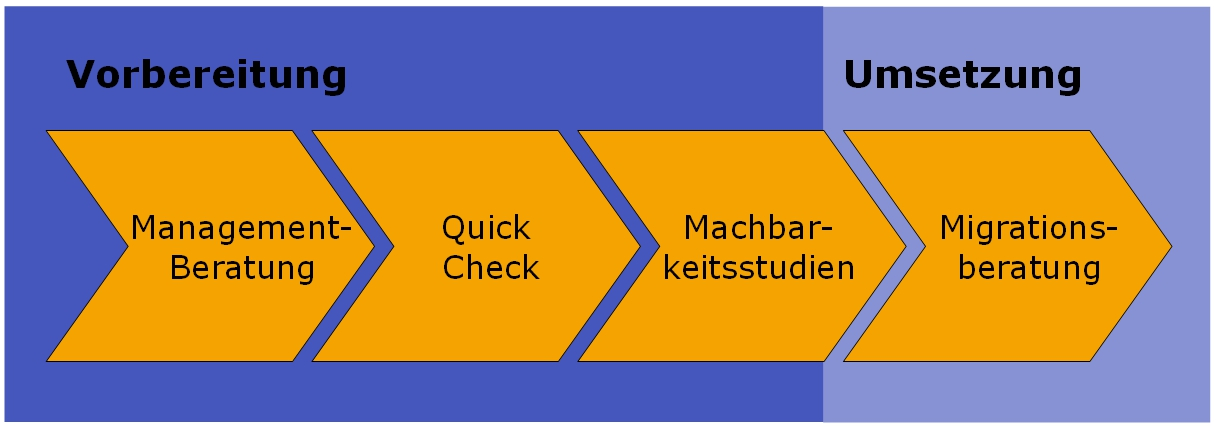
\includegraphics[width=6.5484in,height=1.9701in]{freiesoftwaredortmund-img2.png}
\par}


\bigskip

{\selectlanguage{ngerman}
Dar\"uber hinaus hat die Beauftragte der Bundesregierung f\"ur
Informationstechnik einen {\quotedblbase}Leitfaden f\"ur die Migration
von Software (Stand M\"arz
2012){\textquotedblleft}\footnote{\ \url{http://www.cio.bund.de/SharedDocs/Kurzmeldungen/DE/2012/20120305_migrationsleitfaden_4_0.html}
[abgerufen am\par \ \ 16.03.2012]} herausgegeben.}

\clearpage{\selectlanguage{ngerman}
\hypertarget{Schlusswort}{}\textbf{7.}\textbf{ }\textbf{Schlusswort}}


\bigskip


\bigskip

{\selectlanguage{ngerman}
F\"ur die st\"adtische Umstellung auf OSS wird zu guter Letzt folgender
schlicht klingender, aber aussagekr\"aftiger Arbeitstitel angeregt:}


\bigskip


\bigskip

{\centering\selectlanguage{ngerman}
\foreignlanguage{english}{\textbf{\textcolor{black}{{\quotedblbase}}}}\foreignlanguage{english}{\textbf{\textcolor{black}{DOSS}}}\foreignlanguage{english}{\textbf{\textcolor{black}{
--
}}}\foreignlanguage{english}{\textbf{\textcolor{black}{Dortmunds}}}\foreignlanguage{english}{\textbf{\textcolor{black}{
}}}\foreignlanguage{english}{\textbf{\textcolor{black}{Open}}}\foreignlanguage{english}{\textbf{\textcolor{black}{
}}}\foreignlanguage{english}{\textbf{\textcolor{black}{Source}}}\foreignlanguage{english}{\textbf{\textcolor{black}{
}}}\foreignlanguage{english}{\textbf{\textcolor{black}{Software}}}\foreignlanguage{english}{\textbf{\textcolor{black}{{\textquotedblleft}}}}
\par}


\bigskip


\bigskip

{\selectlanguage{ngerman}
\textcolor{black}{Abschlie{\ss}end eine pers\"onliche Bemerkung:
Unabh\"angigkeit von den M\"arkten ist (besonders in diesen Tagen) ein
unverzichtbarer Bestandteil verantwortlichen Verwaltungshandelns.
Verwaltung muss agieren, statt nur zu reagieren. Der skizzierte
L\"osungsvorschlag soll hierzu dienen!}}

\clearpage{\selectlanguage{ngerman}\bfseries
\hypertarget{Lizenzhinweis}{}Lizenzhinweis}


\bigskip


\bigskip

{\centering 

\includegraphics[width=1.222in,height=0.4307in]{freiesoftwaredortmund-img3.png}
\par}


\bigskip

{\selectlanguage{ngerman}
\textcolor{black}{{\quotedblbase}}\textcolor{black}{Open}\textcolor{black}{
}\textcolor{black}{Source}\textcolor{black}{
}\textcolor{black}{Software}\textcolor{black}{
}\textcolor{black}{im}\textcolor{black}{
}\textcolor{black}{gesch\"aftskritischen}\textcolor{black}{
}\textcolor{black}{Einsatz}\textcolor{black}{
}\textcolor{black}{bei}\textcolor{black}{
}\textcolor{black}{der}\textcolor{black}{
}\textcolor{black}{Stadt}\textcolor{black}{
}\textcolor{black}{Dortmund}\textcolor{black}{{\textquotedblleft}
erstellt am 30.04.2012 }\textcolor{black}{von}\textcolor{black}{
}\textcolor{black}{Christian}\textcolor{black}{
}\textcolor{black}{N\"ahle}\textcolor{black}{
}\textcolor{black}{steht}\textcolor{black}{
}\textcolor{black}{unter}\textcolor{black}{
}\textcolor{black}{einer}\textcolor{black}{
}\href{http://creativecommons.org/licenses/by-sa/3.0/de/}{\textstyleInternetlink{Creative}}\href{http://creativecommons.org/licenses/by-sa/3.0/de/}{\textstyleInternetlink{
}}\href{http://creativecommons.org/licenses/by-sa/3.0/de/}{\textstyleInternetlink{Commons}}\href{http://creativecommons.org/licenses/by-sa/3.0/de/}{\textstyleInternetlink{
}}\href{http://creativecommons.org/licenses/by-sa/3.0/de/}{\textstyleInternetlink{Namensnennung-Weitergabe}}\href{http://creativecommons.org/licenses/by-sa/3.0/de/}{\textstyleInternetlink{
}}\href{http://creativecommons.org/licenses/by-sa/3.0/de/}{\textstyleInternetlink{unter}}\href{http://creativecommons.org/licenses/by-sa/3.0/de/}{\textstyleInternetlink{
}}\href{http://creativecommons.org/licenses/by-sa/3.0/de/}{\textstyleInternetlink{gleichen}}\href{http://creativecommons.org/licenses/by-sa/3.0/de/}{\textstyleInternetlink{
}}\href{http://creativecommons.org/licenses/by-sa/3.0/de/}{\textstyleInternetlink{Bedingungen}}\href{http://creativecommons.org/licenses/by-sa/3.0/de/}{\textstyleInternetlink{
}}\href{http://creativecommons.org/licenses/by-sa/3.0/de/}{\textstyleInternetlink{3.0}}\href{http://creativecommons.org/licenses/by-sa/3.0/de/}{\textstyleInternetlink{
}}\href{http://creativecommons.org/licenses/by-sa/3.0/de/}{\textstyleInternetlink{Deutschland}}\href{http://creativecommons.org/licenses/by-sa/3.0/de/}{\textstyleInternetlink{
}}\href{http://creativecommons.org/licenses/by-sa/3.0/de/}{\textstyleInternetlink{Lizenz}}\textcolor{black}{.}\footnote{\ \url{http://creativecommons.org/licenses/by-sa/3.0/de/}
[abgerufen am 09.04.2012]}\textcolor{black}{.}}

{\selectlanguage{ngerman}
\textcolor{black}{Der}\textcolor{black}{
}\textcolor{black}{Autor}\textcolor{black}{
}\textcolor{black}{ist}\textcolor{black}{
}\textcolor{black}{per}\textcolor{black}{
}\textcolor{black}{E-Mail}\textcolor{black}{
}\textcolor{black}{erreichbar:}\textcolor{black}{
}\href{mailto:c.naehle@gmx.net}{\textstyleInternetlink{\foreignlanguage{ngerman}{c.naehle@gmx.net}}}}

{\selectlanguage{ngerman}
Im Falle einer Verbreitung m\"ussen Sie anderen alle Lizenzbedingungen
mitteilen, die f\"ur dieses Werk gelten. Dies stellt sicher, dass das
in diesem Text zusammengetragene Wissen von jeder Person stets frei
vervielf\"altigt, kopiert, ver\"andert und somit f\"ur individuelle
Anspr\"uche weiterentwickelt werden darf.}


\bigskip

{\selectlanguage{ngerman}


\includegraphics[width=0.6665in,height=0.6665in]{freiesoftwaredortmund-img4.png}
\textstyleStrongEmphasis{Namensnennung} -- Sie m\"ussen den Namen des
Autors/Rechteinhabers in der von ihm festgelegten Weise nennen.}


\bigskip

{\selectlanguage{ngerman}


\includegraphics[width=0.6665in,height=0.6665in]{freiesoftwaredortmund-img5.png}
\textstyleStrongEmphasis{Weitergabe unter gleichen Bedingungen} -- Wenn
Sie das lizenzierte Werk bzw. den lizenzierten Inhalt bearbeiten oder
in anderer Weise erkennbar als Grundlage f\"ur eigenes Schaffen
verwenden, d\"urfen Sie die daraufhin neu entstandenen Werke bzw.
Inhalte nur unter Verwendung von Lizenzbedingungen weitergeben, die mit
denen dieses Lizenzvertrages identisch oder vergleichbar sind.}

\clearpage{\selectlanguage{ngerman}\bfseries
\hypertarget{Danksagung}{}Danksagung}


\bigskip


\bigskip

{\selectlanguage{ngerman}
Ich danke Till Sch\"afer und Philipp Lewe daf\"ur, dass sie mir Open
Source Software n\"achtelang auf meinem Balkon n\"aher gebracht haben
und mir hilfreich mit Anmerkungen f\"ur den endlich vorliegenden
Verbesserungsvorschlag f\"ur die Stadt Dortmund zur Seite gestanden
haben.}

{\selectlanguage{ngerman}
Gleichen Dank f\"ur wertvolle Anmerkungen schulde ich meinem Bruder
Nicolai Parlog und Church-of-Emacs-Anh\"anger Vlado Plaga.}

{\selectlanguage{ngerman}
Vor meiner Freundin und Lektorin, N. Fresen, verneige ich mich in
tiefster Dankbarkeit f\"ur ihre Unterst\"utzung und ewige Geduld mit
mir!}

\clearpage{\selectlanguage{ngerman}\bfseries
\hypertarget{Literaturliste}{}Literaturliste}


\bigskip


\bigskip

{\selectlanguage{ngerman}
\textstyleInternetlink{\textcolor{black}{Bundesverwaltungsamt: URL:
}}\href{http://www.bva.bund.de/}{\textstyleInternetlink{http://www.bva.bund.de}}
[abgerufen\textstyleInternetlink{\textcolor{black}{ am 22.03.2012]}}}


\bigskip

{\selectlanguage{ngerman}
Bundesverwaltungsamt, Kompetenzzentrum Open Source Software: URL:
\href{https://www.oss.bund.de/node/107}{\textstyleInternetlink{http}}\href{https://www.oss.bund.de/node/107}{\textstyleInternetlink{s://www.oss.bund.de/node/107}}
\foreignlanguage{english}{\textcolor{black}{[abgerufen am
13.03.2012]}}}


\bigskip

{\selectlanguage{ngerman}
\textcolor{black}{Bundesverwaltungsamt, Kompetenzzentrum Open Source
Software: URL:
}\href{https://www.oss.bund.de/node/133}{\textstyleInternetlink{http}}\href{https://www.oss.bund.de/node/133}{\textstyleInternetlink{\foreignlanguage{ngerman}{s}}}\href{https://www.oss.bund.de/node/133}{\textstyleInternetlink{://www.oss.bund.de/node/133}}
\foreignlanguage{english}{\textcolor{black}{[abgerufen am
13.03.2012]}}}


\bigskip

{\selectlanguage{ngerman}
\foreignlanguage{english}{\textcolor{black}{Bu}}\foreignlanguage{english}{\textcolor{black}{ndesverwaltungsamt,
Kompetenzzentrum}}\textcolor{black}{ Open Source
Software}\foreignlanguage{english}{\textcolor{black}{:
{\quotedblbase}Projekt LiMux in M\"unchen{\textquotedblleft}. URL:
}}\url{https://www.oss.bund.de/node/275}\textstyleInternetlink{\textcolor{black}{
}}\textstyleInternetlink{\textcolor{black}{[abgerufen am 13.03.2012]}}}


\bigskip

{\selectlanguage{ngerman}
\textstyleInternetlink{\textcolor{black}{Creative Commons:
{\quotedblbase}Namensnennung-Weitergabe unter gleichen Bedingungen 3.0
Deutschland (CC BY-SA 3.0){\textquotedblleft}. URL:
}}\url{http://creativecommons.org/licenses/by-sa/3.0/de/}\textstyleInternetlink{\textcolor{black}{
[abgerufen am 09.04.2012]}}}


\bigskip

{\selectlanguage{ngerman}
dosys -- IT-Konzept Stadt Dortmund 2011-2015, in der Stadtverwaltung
abgestimmter Entwurf; zur Vorlage im VV am 15.11.2011 und im Ausschuss
f\"ur Personal und Organisation am 22.11.11, Dortmund: Stadt Dortmund,
2011}


\bigskip

{\selectlanguage{ngerman}
Ernst \& Young AG: {\quotedblbase}Open Source Software im
gesch\"aftskritischen Einsatz{\textquotedblleft}, Brosch\"ure, Ernst \&
Young AG, 2011}


\bigskip

{\selectlanguage{ngerman}
\textstyleInternetlink{\textcolor{black}{Die Beauftragte der
Bundesregierung f\"ur Informationstechnik:
{\quotedblbase}Migrationsleitfaden in der Version 4.0
ver\"offentlicht{\textquotedblleft}. URL:
}}\href{http://www.cio.bund.de/SharedDocs/Kurzmeldungen/DE/2012/20120305_migrationsleitfaden_4_0.html}{\textstyleInternetlink{http://www.cio.bund.de/SharedDocs/Kurzmeldungen/DE/2012/}}}

{\selectlanguage{ngerman}
\href{http://www.cio.bund.de/SharedDocs/Kurzmeldungen/DE/2012/20120305_migrationsleitfaden_4_0.html}{\textstyleInternetlink{20120305\_migrationsleitfaden\_4\_0.html}}\textstyleInternetlink{\textcolor{black}{
[abgerufen am }}\textstyleInternetlink{\textcolor{black}{16.03.2012]}}}


\bigskip

{\selectlanguage{ngerman}
\textstyleInternetlink{\textcolor{black}{Free Software Foundation Inc.:
{\quotedblbase}Was ist Freie Software?{\textquotedblleft}. URL:
}}\url{http://www.gnu.org/philosophy/free-sw.de.html}\textstyleInternetlink{\textcolor{black}{
}}\textstyleInternetlink{\textcolor{black}{[abgerufen am 13.03.2012]}}}


\bigskip

{\selectlanguage{ngerman}
GR\"UNE Ratsfraktion: {\quotedblbase}Erg\"anzungsantrag zum IT-Konzept
2011-2015{\textquotedblleft}, Dortmund, GR\"UNE Ratsfraktion,
08.02.2012}

{\selectlanguage{ngerman}
G\"unther, Jochen Dipl.-Wi.-Ing: {\quotedblbase}Open Source Software.
Strukturwandel oder Strohfeuer{\textquotedblleft} In: Spath, Dieter
Prof. Dr.-Ing (Hg.) {\quotedblbase}Open Source Software. Strukturwandel
oder Strohfeuer{\textquotedblleft}, Stuttgart: }

{\selectlanguage{ngerman}
Fraunhofer Institut f\"ur Arbeitswirtschaft und Organisation, 2006}


\bigskip

{\selectlanguage{ngerman}
\textstyleInternetlink{\textcolor{black}{heise online:
{\quotedblbase}}}\textstyleInternetlink{\textcolor{black}{40.000}}\textstyleInternetlink{\textcolor{black}{
}}\textstyleInternetlink{\textcolor{black}{neue}}\textstyleInternetlink{\textcolor{black}{
}}\textstyleInternetlink{\textcolor{black}{Linux-Desktops}}\textstyleInternetlink{\textcolor{black}{
}}\textstyleInternetlink{\textcolor{black}{in}}\textstyleInternetlink{\textcolor{black}{
}}\textstyleInternetlink{\textcolor{black}{Spanien}}\textstyleInternetlink{\textcolor{black}{{\textquotedblleft}}}\textstyleInternetlink{\textcolor{black}{.
URL:
}}\url{http://www.heise.de/open/meldung/40-000-neue-Linux-Desktops-in-Spanien-1419719.html}}

{\selectlanguage{ngerman}
\textstyleInternetlink{\textcolor{black}{[abgerufen am 23.01.2012]}}}


\bigskip

{\selectlanguage{ngerman}
\textstyleInternetlink{\textcolor{black}{heise online:
{\quotedblbase}}}\textstyleInternetlink{\textcolor{black}{Bundeswehr}}\textstyleInternetlink{\textcolor{black}{
}}\textstyleInternetlink{\textcolor{black}{setzt}}\textstyleInternetlink{\textcolor{black}{
}}\textstyleInternetlink{\textcolor{black}{auf}}\textstyleInternetlink{\textcolor{black}{
}}\textstyleInternetlink{\textcolor{black}{Open}}\textstyleInternetlink{\textcolor{black}{
}}\textstyleInternetlink{\textcolor{black}{Source}}\textstyleInternetlink{\textcolor{black}{
}}\textstyleInternetlink{\textcolor{black}{und}}\textstyleInternetlink{\textcolor{black}{
}}\textstyleInternetlink{\textcolor{black}{SOA}}\textstyleInternetlink{\textcolor{black}{{\textquotedblleft}}}\textstyleInternetlink{\textcolor{black}{.
URL:
}}\href{http://www.heise.de/newsticker/meldung/Bundeswehr-setzt-auf-Open-Source-und-SOA-1430186.html}{\textstyleInternetlink{http://www.heise.de/newsticker/meldung/}}}

{\selectlanguage{ngerman}
\href{http://www.heise.de/newsticker/meldung/Bundeswehr-setzt-auf-Open-Source-und-SOA-1430186.html}{\textstyleInternetlink{Bundeswehr-setzt-auf-Open-Source-und-SOA-1430186.html}}\textstyleInternetlink{\textcolor{black}{
}}\foreignlanguage{english}{\textcolor{black}{[abgerufen am
07.02.2012]}}}


\bigskip

{\selectlanguage{ngerman}
\textstyleInternetlink{\textcolor{black}{heise online:
{\quotedblbase}}}\textstyleInternetlink{\textcolor{black}{LiMux:}}\textstyleInternetlink{\textcolor{black}{
}}\textstyleInternetlink{\textcolor{black}{Billiger}}\textstyleInternetlink{\textcolor{black}{
}}\textstyleInternetlink{\textcolor{black}{und}}\textstyleInternetlink{\textcolor{black}{
}}\textstyleInternetlink{\textcolor{black}{robuster}}\textstyleInternetlink{\textcolor{black}{
}}\textstyleInternetlink{\textcolor{black}{als}}\textstyleInternetlink{\textcolor{black}{
}}\textstyleInternetlink{\textcolor{black}{Windows}}\textstyleInternetlink{\textcolor{black}{{\textquotedblleft}}}\textstyleInternetlink{\textcolor{black}{.
URL:
}}\url{http://www.heise.de/open/meldung/LiMux-Billiger-und-robuster-als-Windows-1485410.html}}

{\selectlanguage{ngerman}
\textstyleInternetlink{\textcolor{black}{[abgerufen am 07.04.2012]}}}


\bigskip

{\selectlanguage{ngerman}
\textstyleInternetlink{\textcolor{black}{heise online:
{\quotedblbase}Nieders\"achsische Steuerverwaltung stellt auf Linux
um{\textquotedblleft}. URL:
}}\href{http://www.heise.de/open/meldung/Niedersaechsische-Steuerverwaltung-stellt-auf-Linux-um-128541.html}{\textstyleInternetlink{http://www.heise.de/open/meldung/}}}

{\selectlanguage{ngerman}
\href{http://www.heise.de/open/meldung/Niedersaechsische-Steuerverwaltung-stellt-auf-Linux-um-128541.html}{\textstyleInternetlink{Niedersaechsische-Steuerverwaltung-stellt-auf-Linux-um-128541.html}}\textstyleInternetlink{\textcolor{black}{
}}\textcolor{black}{[abgerufen am
}\foreignlanguage{english}{\textcolor{black}{13.03.2012]}}}


\bigskip

{\selectlanguage{ngerman}
\textstyleInternetlink{\textcolor{black}{heise online:
{\quotedblbase}}}\textstyleInternetlink{\textcolor{black}{Open}}\textstyleInternetlink{\textcolor{black}{
}}\textstyleInternetlink{\textcolor{black}{Source}}\textstyleInternetlink{\textcolor{black}{
}}\textstyleInternetlink{\textcolor{black}{f\"ur}}\textstyleInternetlink{\textcolor{black}{
}}\textstyleInternetlink{\textcolor{black}{New}}\textstyleInternetlink{\textcolor{black}{
}}\textstyleInternetlink{\textcolor{black}{Hampshire}}\textstyleInternetlink{\textcolor{black}{{\textquotedblleft}}}\textstyleInternetlink{\textcolor{black}{.
URL:
}}\href{http://www.heise.de/open/meldung/Open-Source-fuer-New-Hampshire-1431833.html}{\textstyleInternetlink{http://www.heise.de/open/meldung/}}}

{\selectlanguage{ngerman}
\href{http://www.heise.de/open/meldung/Open-Source-fuer-New-Hampshire-1431833.html}{\textstyleInternetlink{Open-Source-fuer-New-Hampshire-1431833.html}}\textstyleInternetlink{\textcolor{black}{
[abgerufen am 09.02.2012]}}}


\bigskip

{\selectlanguage{ngerman}
\textstyleInternetlink{\textcolor{black}{heise online:
{\quotedblbase}Studie: Open-Source-Software qualitativ besser als
propriet\"are Entwicklungen{\textquotedblleft}. URL:
}}\url{http://heise.de/-1440788}\textstyleInternetlink{\textcolor{black}{
}}\textstyleInternetlink{\textcolor{black}{[abgerufen am
}}\textstyleInternetlink{\textcolor{black}{13.03.2012]}}}


\bigskip

{\selectlanguage{ngerman}
\textstyleInternetlink{\textcolor{black}{Huber, Mathias (2012):
{\quotedblbase}}}\textstyleInternetlink{\textcolor{black}{Enterprise-Anwender}}\textstyleInternetlink{\textcolor{black}{
}}\textstyleInternetlink{\textcolor{black}{setzen}}\textstyleInternetlink{\textcolor{black}{
}}\textstyleInternetlink{\textcolor{black}{auf}}\textstyleInternetlink{\textcolor{black}{
}}\textstyleInternetlink{\textcolor{black}{Linux}}\textstyleInternetlink{\textcolor{black}{
}}\textstyleInternetlink{\textcolor{black}{f\"ur}}\textstyleInternetlink{\textcolor{black}{
}}\textstyleInternetlink{\textcolor{black}{Big}}\textstyleInternetlink{\textcolor{black}{
}}\textstyleInternetlink{\textcolor{black}{Data}}\textstyleInternetlink{\textcolor{black}{{\textquotedblleft}.}}\textstyleInternetlink{\textcolor{black}{
}}}

{\selectlanguage{ngerman}
\textstyleInternetlink{\textcolor{black}{URL:
}}\url{http://www.linux-magazin.de/NEWS/Enterprise-Anwender-setzen-auf-Linux-fuer-Big-Data}\textstyleInternetlink{\textcolor{black}{
}}\textstyleInternetlink{\textcolor{black}{[abgerufen am 15.03.2012]}}}


\bigskip

{\selectlanguage{ngerman}
Kaczmarek, Oliver und andere Abgeordnete der SPD Bundestagsfraktion:
{\quotedblbase}Kleine Anfrage. Sachstand zur Nutzung von
{\quotesinglbase}freier Software{\textquoteleft} im Ausw\"artigen Amt
und weiteren Bundesbeh\"orden.{\textquotedblleft} Elektronische
Vorabfassung, Berlin: H. Heenemann GmbH \& Co., 26.01.2011}


\bigskip

{\selectlanguage{ngerman}
\textcolor{black}{Kiefer,
Bernd}\textcolor{black}{{}-Uwe:}\textcolor{black}{
{\quotedblbase}}\textcolor{black}{FUM}\textcolor{black}{
}\textcolor{black}{08}\textcolor{black}{.
}\textstyleInternetlink{\textcolor{black}{F\"uhrungsaspekte}}\textstyleInternetlink{\textcolor{black}{
}}\textstyleInternetlink{\textcolor{black}{des}}\textstyleInternetlink{\textcolor{black}{
}}\textstyleInternetlink{\textcolor{black}{Projektmanagements}}\textstyleInternetlink{\textcolor{black}{{\textquotedblleft}}}\textstyleInternetlink{\foreignlanguage{ngerman}{\textcolor{black}{.}}}\textstyleInternetlink{\foreignlanguage{ngerman}{\textcolor{black}{
}}}\textstyleInternetlink{\foreignlanguage{ngerman}{\textcolor{black}{Pfungstadt:}}}\textstyleInternetlink{\foreignlanguage{ngerman}{\textcolor{black}{
}}}\textcolor{black}{Studiengemeinschaft}\textcolor{black}{
}\textcolor{black}{Werner}\textcolor{black}{
}\textcolor{black}{Kamprath}\textcolor{black}{
}\textcolor{black}{Darmstadt}\textcolor{black}{
}\textcolor{black}{GmbH}\textcolor{black}{, 2012}}


\bigskip

{\selectlanguage{ngerman}
\textstyleInternetlink{\textcolor{black}{Laufer, Simon (2011):
{\quotedblbase}}}\textstyleInternetlink{\textcolor{black}{20 Jahre
Linux}}\textstyleInternetlink{\foreignlanguage{ngerman}{\textcolor{black}{.
}}}\textstyleInternetlink{\textcolor{black}{Wie}}\textstyleInternetlink{\textcolor{black}{
}}\textstyleInternetlink{\textcolor{black}{der}}\textstyleInternetlink{\textcolor{black}{
}}\textstyleInternetlink{\textcolor{black}{Pinguin}}\textstyleInternetlink{\textcolor{black}{
}}\textstyleInternetlink{\textcolor{black}{nach}}\textstyleInternetlink{\textcolor{black}{
}}\textstyleInternetlink{\textcolor{black}{M\"unchen}}\textstyleInternetlink{\textcolor{black}{
}}\textstyleInternetlink{\textcolor{black}{kam}}\textstyleInternetlink{\textcolor{black}{{\textquotedblleft}.
URL:}}\textstyleInternetlink{\textcolor{black}{
}}\url{http://www.spiegel.de/netzwelt/web/0,1518,781680,00.html}
\textstyleInternetlink{\textcolor{black}{[abgerufen am 13.03.2012]}}}


\bigskip

{\selectlanguage{ngerman}
\textstyleInternetlink{\foreignlanguage{ngerman}{\textcolor{black}{Norddeutscher
Rundfunk}}}\textstyleInternetlink{\textcolor{black}{:
{\quotedblbase}Deutschland bleibt IT-Mittelma{\ss}{\textquotedblleft}.
URL:
}}\url{http://www.tagesschau.de/inland/itgipfel120.html}\textstyleInternetlink{\textcolor{black}{
[abgerufen am 09.04.2012]}}}


\bigskip

{\selectlanguage{ngerman}
\foreignlanguage{english}{Renner,}\foreignlanguage{english}{
}\foreignlanguage{english}{Thomas}\foreignlanguage{english}{
}\foreignlanguage{english}{et}\foreignlanguage{english}{
}\foreignlanguage{english}{al.:}\foreignlanguage{english}{
{\quotedblbase}}\foreignlanguage{english}{Open}\foreignlanguage{english}{
}\foreignlanguage{english}{Source}\foreignlanguage{english}{
}\foreignlanguage{english}{Software}\foreignlanguage{english}{.
}Einsparpotentiale und Wirtschaftlichkeit{\textquotedblright}.
Stuttgart: }

{\selectlanguage{ngerman}
Fraunhofer Institut f\"ur Arbeitswirtschaft und Organisation, 2005}


\bigskip

{\selectlanguage{ngerman}
\textstyleInternetlink{\foreignlanguage{ngerman}{\textcolor{black}{Stadt}}}\textstyleInternetlink{\foreignlanguage{ngerman}{\textcolor{black}{
}}}\textstyleInternetlink{\foreignlanguage{ngerman}{\textcolor{black}{Dortmund}}}\textstyleInternetlink{\foreignlanguage{ngerman}{\textcolor{black}{
}}}\textstyleInternetlink{\foreignlanguage{ngerman}{\textcolor{black}{(Hg):}}}\textstyleInternetlink{\foreignlanguage{ngerman}{\textcolor{black}{
}}}\textstyleInternetlink{\textcolor{black}{{\quotedblbase}}}\textstyleInternetlink{\textcolor{black}{MAI}}\textstyleInternetlink{\foreignlanguage{ngerman}{\textcolor{black}{.}}}\textstyleInternetlink{\foreignlanguage{ngerman}{\textcolor{black}{
}}}\textstyleInternetlink{\textcolor{black}{Mitarbeiterinnen-}}\textstyleInternetlink{\textcolor{black}{
}}\textstyleInternetlink{\textcolor{black}{und}}\textstyleInternetlink{\textcolor{black}{
}}\textstyleInternetlink{\textcolor{black}{Mitarbeiterinformation}}\textstyleInternetlink{\foreignlanguage{ngerman}{\textcolor{black}{{\textquotedblleft}}}}\textstyleInternetlink{\textcolor{black}{,}}\textstyleInternetlink{\textcolor{black}{
}}\textstyleInternetlink{\textcolor{black}{Nr.}}\textstyleInternetlink{\textcolor{black}{
}}\textstyleInternetlink{\textcolor{black}{3}}\textstyleInternetlink{\foreignlanguage{ngerman}{\textcolor{black}{/2011}}}\textstyleInternetlink{\textcolor{black}{,}}\textstyleInternetlink{\textcolor{black}{
}}\textstyleInternetlink{\foreignlanguage{ngerman}{\textcolor{black}{Dortmund:
Stadt Dortmund,
}}}\textstyleInternetlink{\textcolor{black}{2011,}}\textstyleInternetlink{\textcolor{black}{
}}\textstyleInternetlink{\textcolor{black}{S.}}\textstyleInternetlink{\textcolor{black}{
}}\textstyleInternetlink{\foreignlanguage{ngerman}{\textcolor{black}{6}}}}


\bigskip

{\selectlanguage{ngerman}
\textstyleInternetlink{\textcolor{black}{Wikimedia}}\textstyleInternetlink{\textcolor{black}{
}}\textstyleInternetlink{\textcolor{black}{Foundation}}\textstyleInternetlink{\textcolor{black}{
}}\textstyleInternetlink{\textcolor{black}{Inc.:}}\textstyleInternetlink{\textcolor{black}{
{\quotedblbase}}}\textstyleInternetlink{\textcolor{black}{Datei:Opensource.svg}}\textstyleInternetlink{\textcolor{black}{{\textquotedblleft}}}\textstyleInternetlink{\textcolor{black}{.}}\textstyleInternetlink{\textcolor{black}{
}}\textstyleInternetlink{\textcolor{black}{URL:}}\textstyleInternetlink{\textcolor{black}{
}}\url{https://de.wikipedia.org/w/index.php?title=Datei:Opensource.svg&filetimestamp=20070822051640}\textstyleInternetlink{\textcolor{black}{
}}\textcolor{black}{[abgerufen}\textcolor{black}{
}\textcolor{black}{am}\textcolor{black}{
}\textcolor{black}{13.03.2012]}}


\bigskip

{\selectlanguage{ngerman}
\textstyleInternetlink{\textcolor{black}{Wikimedia Foundation Inc.:
{\quotedblbase}Digitale Kluft{\textquotedblleft}. URL:
}}\url{https://de.wikipedia.org/wiki/Digitale_Kluft}\textstyleInternetlink{\textcolor{black}{
[abgerufen am 13.03.2012]}}}


\bigskip

{\selectlanguage{ngerman}
\textstyleInternetlink{\textcolor{black}{Wikimedia Foundation Inc.:
{\quotedblbase}Kompilierung{\textquotedblleft}. URL:
}}\url{https://de.wikipedia.org/wiki/Kompilierung}}

{\selectlanguage{ngerman}
\textstyleInternetlink{\textcolor{black}{[abgerufen am 13.03.2012]}}}


\bigskip

{\selectlanguage{ngerman}
\textstyleInternetlink{\textcolor{black}{Wikimedia Foundation Inc.:
{\quotedblbase}Know-how{\textquotedblleft}. URL:
}}\url{https://de.wikipedia.org/wiki/Know-how}}

{\selectlanguage{ngerman}
\textstyleInternetlink{\textcolor{black}{[abgerufen am 22.03.2012]}}}


\bigskip

{\selectlanguage{ngerman}
\textstyleInternetlink{\textcolor{black}{Wikimedia Foundation Inc.:
{\quotedblbase}Offener Standard{\textquotedblleft}.
URL:}}\textstyleInternetlink{\foreignlanguage{ngerman}{\textcolor{black}{
}}}\url{https://de.wikipedia.org/wiki/Offener_Standard}\textstyleInternetlink{\textcolor{black}{
}}\textcolor{black}{[abgerufen am 13.03.2012]}}


\bigskip

{\selectlanguage{ngerman}
\foreignlanguage{english}{\textcolor{black}{Wikimedia Foundation Inc.:
{\quotedblbase}Open Source{\textquotedblleft}. URL:
}}\href{https://de.wikipedia.org/wiki/Open_Source#Begriffsproblem_.E2.80.9EFreie_Software.E2.80.9C
}{\textstyleInternetlink{https://de.wikipedia.org/wiki/Open\_Source\#Begriffsproblem\_.E2.80.9EFreie\_Software.E2.80.9C}}\foreignlanguage{english}{\textcolor{black}{
[abgerufen am 13.03.2012]}}}


\bigskip

{\selectlanguage{ngerman}
\textstyleInternetlink{\textcolor{black}{Wikimedia Foundation Inc.:
{\quotedblbase}Open-Source-Software in \"offentlichen
Einrichtungen{\textquotedblleft}.
URL:}}\textstyleInternetlink{\foreignlanguage{english}{\textcolor{black}{
}}}\href{https://de.wikipedia.org/wiki/Open-Source-Software_in_?ffentlichen_Einrichtungen}{\textstyleInternetlink{https://de.wikipedia.org/wiki/Open-Source-Software\_in\_\%C3\%B6ffentlichen\_Einrichtungen}}}

{\selectlanguage{ngerman}
\textstyleInternetlink{\textcolor{black}{[abgerufen am 05.03.2012]}}}

{\selectlanguage{ngerman}
\textstyleInternetlink{\textcolor{black}{Wikimedia Foundation Inc.:
{\quotedblbase}Propriet\"are Software{\textquotedblleft}. URL:
}}\href{https://de.wikipedia.org/wiki/Propriet?re_Software}{\textstyleInternetlink{https://de.wikipedia.org/wiki/Propriet\%C3\%A4re\_Software}}\textstyleInternetlink{\textcolor{black}{
}}\textcolor{black}{[abgerufen am 13.03.2012]}}


\bigskip

{\selectlanguage{ngerman}
\textstyleInternetlink{\textcolor{black}{Wikimedia}}\textstyleInternetlink{\textcolor{black}{
}}\textstyleInternetlink{\textcolor{black}{Foundation}}\textstyleInternetlink{\textcolor{black}{
}}\textstyleInternetlink{\textcolor{black}{Inc.:}}\textstyleInternetlink{\textcolor{black}{
{\quotedblbase}}}\textstyleInternetlink{\textcolor{black}{Quelltext}}\textstyleInternetlink{\textcolor{black}{{\textquotedblleft}}}\textstyleInternetlink{\textcolor{black}{.}}\textstyleInternetlink{\textcolor{black}{
}}\textstyleInternetlink{\textcolor{black}{URL:}}\textstyleInternetlink{\textcolor{black}{
}}\url{https://de.wikipedia.org/wiki/Quelltext}}

{\selectlanguage{english}\color{black}
[abgerufen am 07.04.2012]}


\bigskip

{\selectlanguage{ngerman}
\textstyleInternetlink{\textcolor{black}{Wikimedia Foundation Inc.:
{\quotedblbase}Red Hat{\textquotedblleft}. URL:
}}\url{https://de.wikipedia.org/wiki/Red_Hat}}

{\selectlanguage{english}\color{black}
[abgerufen am 13.03.2012]}


\bigskip

{\selectlanguage{ngerman}
\textstyleInternetlink{\textcolor{black}{Wikimedia Foundation Inc.:
{\quotedblbase}Softwarepatent{\textquotedblleft}. URL:
}}\url{https://de.wikipedia.org/wiki/Softwarepatent#Europ.C3.A4ische_Union}}

{\selectlanguage{ngerman}\color{black}
[abgerufen am 16.03 2012]}


\bigskip

{\selectlanguage{ngerman}
\textstyleInternetlink{\textcolor{black}{Wikimedia Foundation Inc.:
{\quotedblbase}Vier-Augen-Prinzip{\textquotedblleft}. URL:
}}\href{https://de.wikipedia.org/wiki/Vier-Augen-Prinzip}{\textstyleInternetlink{https://de.wikipedia.org/wiki/}}}

{\selectlanguage{ngerman}
\href{https://de.wikipedia.org/wiki/Vier-Augen-Prinzip}{\textstyleInternetlink{Vier-Augen-Prinzip}}\textstyleInternetlink{\textcolor{black}{
}}\textcolor{black}{[abgerufen am 13.03.2012]}}
\end{document}
